% ============================================================
% AeroTrack Lab Report - Blockchain Engineering
% ============================================================
\documentclass[12pt,a4paper]{article}

% --- Encoding and Fonts ---
\usepackage[utf8]{inputenc}
\usepackage[T1]{fontenc}
\usepackage{lmodern}

% --- Page Layout ---
\usepackage[margin=2.5cm,headheight=14pt]{geometry}

% --- Graphics and Colors ---
\usepackage{graphicx}
\usepackage{xcolor}
\usepackage{float}

% --- Tables ---
\usepackage{booktabs}
\usepackage{tabularx}

% --- Section Styling ---
\usepackage{titlesec}
\titleformat{\section}{\Large\bfseries\color{blue!70!black}}{\thesection}{1em}{}[\vspace{-0.5em}\rule{\textwidth}{0.4pt}]
\titleformat{\subsection}{\large\bfseries\color{blue!50!black}}{\thesubsection}{1em}{}

% --- Code Listings ---
\usepackage{listings}

% Define Solidity language for listings
\lstdefinelanguage{Solidity}{
    keywords={pragma, solidity, contract, function, modifier, event, emit, require, mapping, struct, enum, public, private, internal, external, memory, storage, returns, return, address, uint256, uint, bool, string, true, false, if, else, for, while, new, delete, constructor, indexed, abstract, interface, library, is, using, view, pure, payable, override, virtual},
    keywordstyle=\color{blue}\bfseries,
    ndkeywords={msg, sender, block, timestamp, this, PartStatus, Part},
    ndkeywordstyle=\color{purple}\bfseries,
    sensitive=true,
    comment=[l]{//},
    morecomment=[s]{/*}{*/},
    commentstyle=\color{gray}\ttfamily,
    stringstyle=\color{red},
    morestring=[b]",
    morestring=[b]'
}

\lstset{
    language=Solidity,
    backgroundcolor=\color{gray!8},
    basicstyle=\footnotesize\ttfamily,
    breaklines=true,
    frame=leftline,
    framesep=8pt,
    framerule=2pt,
    rulecolor=\color{blue!40},
    numbers=left,
    numberstyle=\tiny\color{gray},
    numbersep=10pt,
    tabsize=4,
    showstringspaces=false,
    captionpos=b,
    aboveskip=12pt,
    belowskip=12pt,
    xleftmargin=15pt
}

% --- Headers and Footers ---
\usepackage{fancyhdr}
\pagestyle{fancy}
\fancyhf{}
\fancyhead[L]{\small\textit{AeroTrack -- Blockchain Lab Report}}
\fancyhead[R]{\small\thepage}
\fancyfoot[L]{\small\textit{Noaman Makhlouf}}
\fancyfoot[R]{\small ENSEM -- S4 2025/2026}
\renewcommand{\headrulewidth}{0.4pt}
\renewcommand{\footrulewidth}{0.4pt}

% --- Hyperlinks (load LAST) ---
\usepackage{hyperref}
\hypersetup{
    colorlinks=true,
    linkcolor=blue!70!black,
    urlcolor=blue!70!black,
    citecolor=blue!70!black
}

% ============================================================
\begin{document}

% --- Title Page ---
\begin{titlepage}
    \centering
    \vspace*{1cm}

    % University header
    \rule{\textwidth}{1.5pt}\\[0.4cm]
    {\LARGE\bfseries ENSEM}\\[0.2cm]
    {\large Ecole Nationale Sup\'erieure d'Electricit\'e et de M\'ecanique}\\[0.1cm]
    {\normalsize Universit\'e Hassan II de Casablanca}\\[0.3cm]
    \rule{\textwidth}{1.5pt}

    \vspace{0.8cm}
    
\includegraphics[width=0.25\textwidth]{logo_ensem.jpg}
    \vspace{0.8cm}

    % Project title
    {\fontsize{28}{34}\selectfont\bfseries Project AeroTrack\par}
    \vspace{0.6cm}
    {\Large\itshape Securing Airplane Spare Parts Provenance\\using Ethereum Smart Contracts\par}

    \vspace{1.2cm}

    % Decorative line
    \rule{0.6\textwidth}{0.4pt}

    \vspace{1.2cm}

    % Info box
    \begin{tabular}{rl}
        \textbf{Module:} & Blockchain Tools \& Applications \\[0.2cm]
        \textbf{Semester:} & S4 -- 2025/2026 \\[0.2cm]
        \textbf{Student:} & Noaman Makhlouf \\[0.2cm]
        \textbf{Supervisor:} & Prof. Khalid Boukhdir \\
    \end{tabular}

    \vfill

    % Footer
    \rule{0.4\textwidth}{0.4pt}\\[0.3cm]
    {\large May 2026}
\end{titlepage}

% --- Table of Contents ---
\newpage
\tableofcontents
\newpage

% ============================================================
\section{Introduction}
% ============================================================

\subsection{Industrial Context}

In the aviation industry, \textbf{dependability and safety} are paramount. A single counterfeit or poorly maintained spare part can compromise the integrity of an entire aircraft. Traditional supply chains rely on centralized databases and paper-based certificates (such as the EASA Form~1 or FAA 8130-3), which are susceptible to forgery, loss, and data manipulation.

\subsection{The Blockchain Solution}

By leveraging \textbf{Ethereum smart contracts}, we can create an immutable, transparent, and decentralized ledger for tracking the lifecycle of airplane parts. From manufacturing through ownership transfers to maintenance logging, every action is cryptographically secured and permanently recorded.

\subsection{Lab Objectives}

This project aims to:
\begin{itemize}
    \item Understand the role of blockchain in industrial supply chain security
    \item Apply Solidity concepts (Structs, Mappings, Modifiers, Events) to a real-world problem
    \item Implement Role-Based Access Control (RBAC)
    \item Deploy, test, and debug a smart contract using Remix IDE
\end{itemize}

% ============================================================
\section{Technical Background}
% ============================================================

\subsection{Ethereum and Smart Contracts}

\textbf{Ethereum} is a decentralized platform that enables developers to deploy self-executing programs called \textbf{smart contracts}. Once deployed, a smart contract's code cannot be modified, ensuring trust and transparency.

\subsection{Key Solidity Concepts}

\begin{table}[H]
\centering
\begin{tabularx}{\textwidth}{lX}
\toprule
\textbf{Concept} & \textbf{Description} \\
\midrule
State Variables & Data stored permanently on the blockchain \\
Structs & Custom data types grouping related fields \\
Mappings & Hash-table-like structures for O(1) key-value access \\
\texttt{msg.sender} & The Ethereum address calling the current function \\
Modifiers & Reusable precondition checks attached to functions \\
Events & Cheap log entries for off-chain traceability \\
\bottomrule
\end{tabularx}
\caption{Core Solidity concepts used in AeroTrack}
\end{table}

% ============================================================
\section{Implementation}
% ============================================================

\subsection{Step 1: Data Architecture}

We define the data model using an \textbf{enum} for part lifecycle states and a \textbf{struct} for part attributes.

\begin{lstlisting}[caption={Part status enum and struct definition}]
enum PartStatus { Manufactured, InTransit, Installed, Retired }

struct Part {
    uint256 serialNumber;
    string partName;
    address manufacturer;
    address currentOwner;
    PartStatus status;
    bool exists;  // Security flag
}
\end{lstlisting}

The \texttt{exists} boolean is a security pattern: since Solidity mappings return default zero-values for non-existent keys, this flag distinguishes between a real part and an empty struct.

\subsubsection{State Transition Graph}
The lifecycle of an airplane part is governed by the \texttt{PartStatus} state machine shown in Figure~\ref{fig:state-machine}:

\begin{figure}[H]
\centering
\begin{verbatim}
[ Manufactured ]  ----(transferPart)--->  [ InTransit ]
       ^                                         |
       |                                   (logMaintenance)
       |                                         v
 [   Retired    ]  <----------------------  [ Installed ]
\end{verbatim}
\caption{AeroTrack part state transitions}
\label{fig:state-machine}
\end{figure}

The \textbf{mapping} provides instant access to any part by its serial number:

\begin{lstlisting}[caption={State variables}]
address public regulatoryAuthority;
mapping(uint256 => Part) public parts;
\end{lstlisting}

After compiling and deploying the contract skeleton on Remix VM, the deployment succeeds as shown in Figure~\ref{fig:step1-deploy}.

\begin{figure}[H]
    \centering
    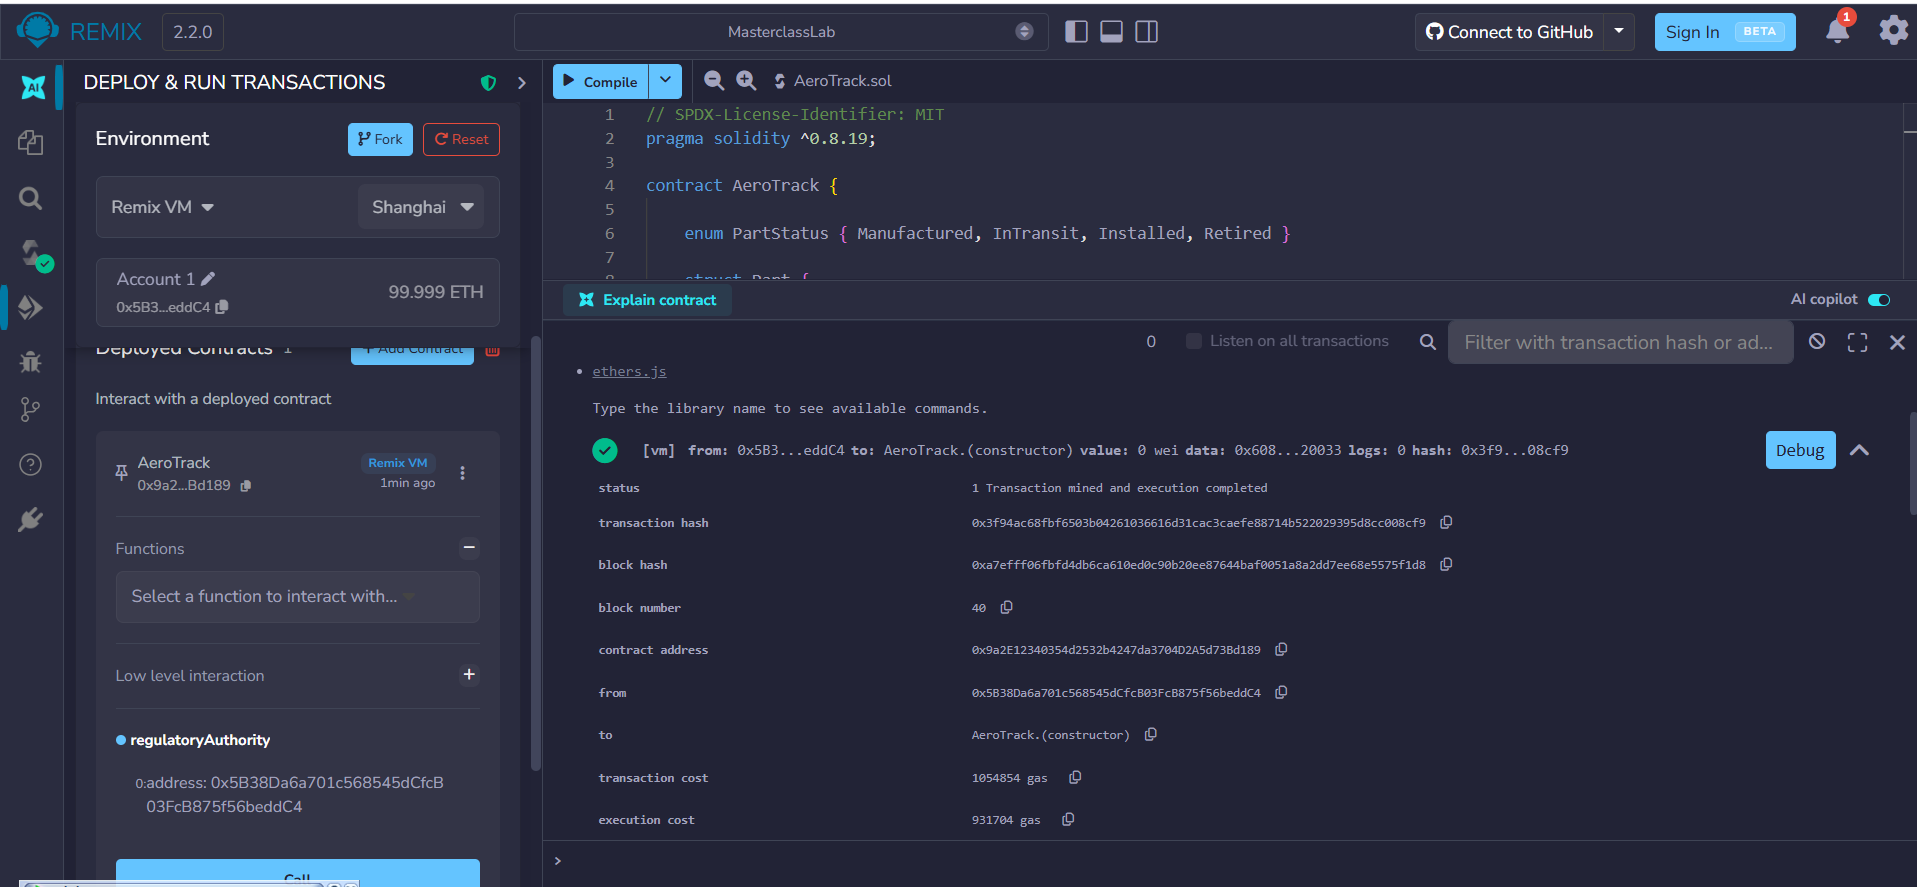
\includegraphics[width=0.85\textwidth]{../screens/step1-deploy-success.png}
    \caption{Successful deployment of the AeroTrack contract on Remix VM}
    \label{fig:step1-deploy}
\end{figure}

Calling the \texttt{regulatoryAuthority} getter confirms that the deployer's address is correctly stored (Figure~\ref{fig:step1-authority}).

\begin{figure}[H]
    \centering
    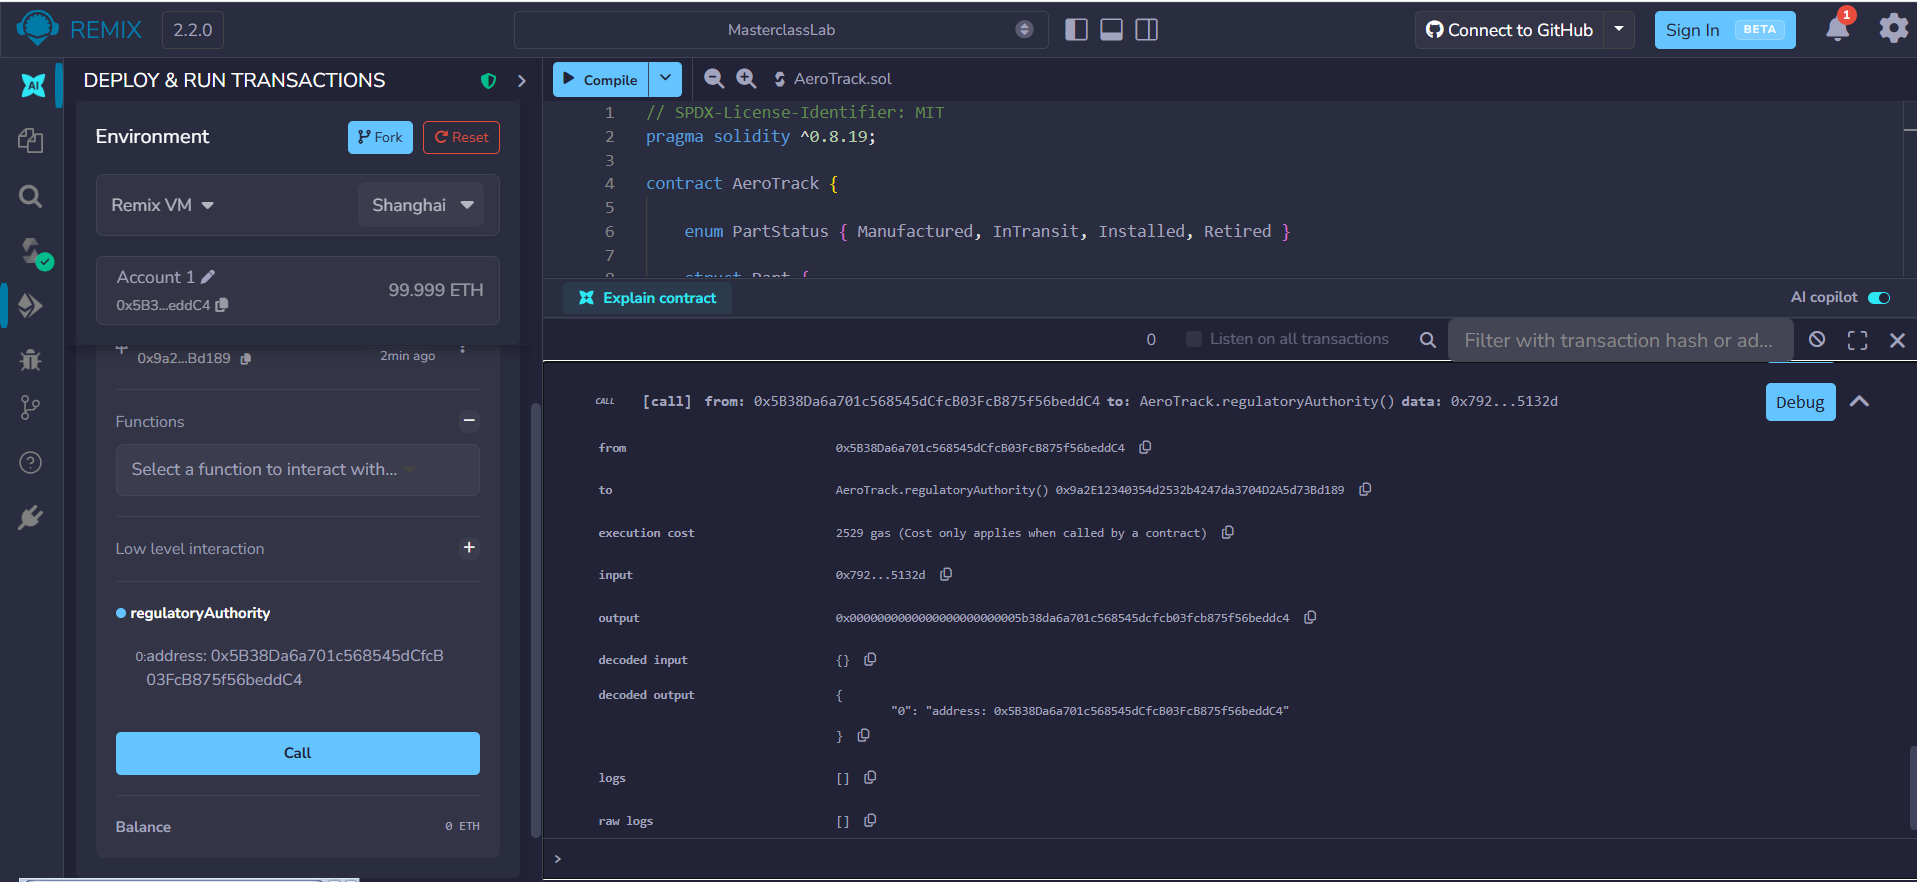
\includegraphics[width=0.85\textwidth]{../screens/step1-regulatoryAuthority-call.png}
    \caption{Querying \texttt{regulatoryAuthority} returns the deployer's address}
    \label{fig:step1-authority}
\end{figure}

\subsubsection{Alignment with Aerospace Regulations}
In legacy aviation supply chains, spare parts are tracked using paper certificates such as the EASA Form 1 (in Europe) or the FAA Form 8130-3 (in the USA). Our digital \texttt{Part} struct directly digitizes the required fields of these forms:
\begin{itemize}
    \item \texttt{serialNumber} corresponds to block 12 (Serial Number) on the FAA 8130-3 form.
    \item \texttt{partName} corresponds to block 10 (Part Number/Description).
    \item \texttt{manufacturer} corresponds to block 13a (Authorized Signature/Organization details).
\end{itemize}

\subsection{Step 2: Role-Based Access Control}

Security is enforced through \textbf{modifiers} -- reusable checks that execute before the function body.

\begin{lstlisting}[caption={Security modifiers}]
modifier partExists(uint256 _serialNumber) {
    require(parts[_serialNumber].exists == true,
            "Part does not exist.");
    _;
}

modifier onlyPartOwner(uint256 _serialNumber) {
    require(parts[_serialNumber].currentOwner == msg.sender,
            "Not the owner.");
    _;
}
\end{lstlisting}

The \texttt{\_;} placeholder indicates where the function body is inserted after the checks pass. If \texttt{require()} fails, the entire transaction reverts.

Figure~\ref{fig:step2-code} shows the modifiers implemented in Remix, and Figure~\ref{fig:step2-compile} confirms successful compilation.

\begin{figure}[H]
    \centering
    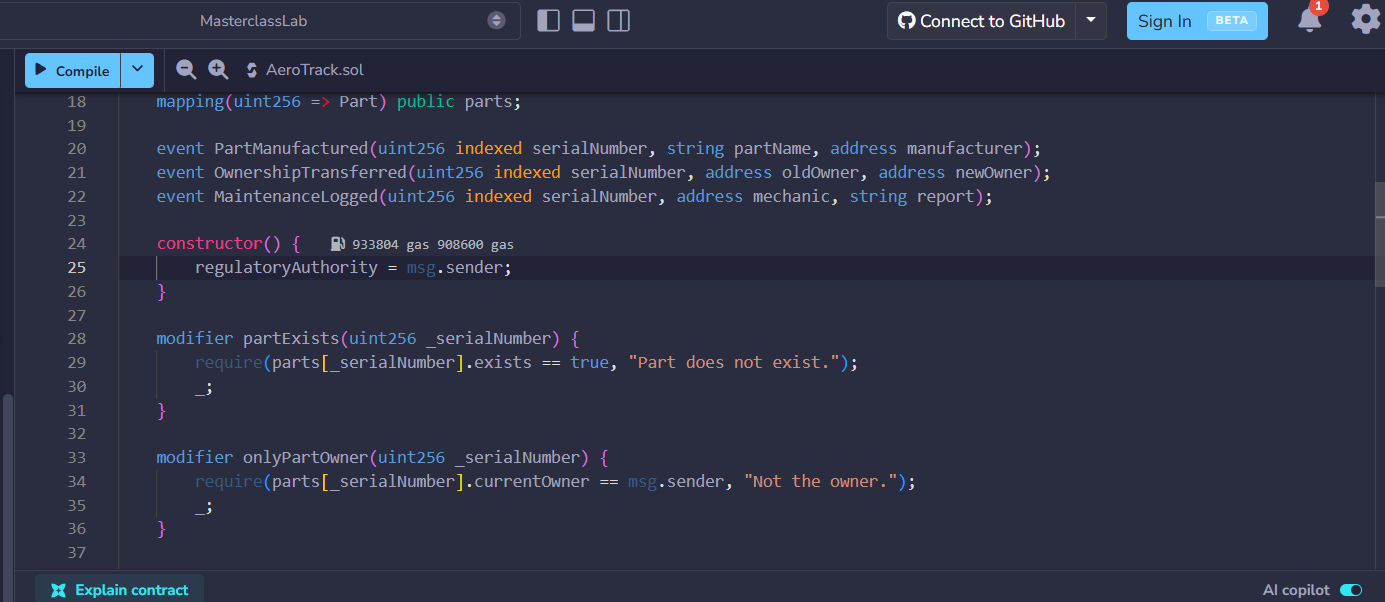
\includegraphics[width=0.85\textwidth]{../screens/step2-modifiers-code.png}
    \caption{Role-based access control modifiers in the Remix editor}
    \label{fig:step2-code}
\end{figure}

\begin{figure}[H]
    \centering
    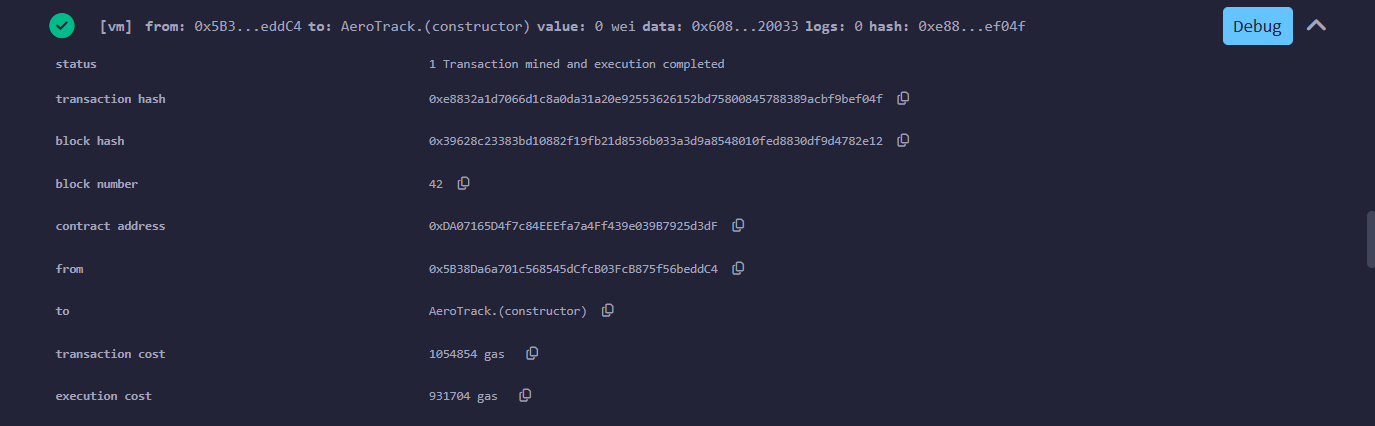
\includegraphics[width=0.85\textwidth]{../screens/step2-compile-success.png}
    \caption{Successful compilation after adding security modifiers}
    \label{fig:step2-compile}
\end{figure}

\subsection{Step 3: Core Business Functions}

\subsubsection{Manufacturing a Part}

\begin{lstlisting}[caption={manufacturePart function}]
function manufacturePart(uint256 _serialNumber,
                         string memory _partName) public {
    require(parts[_serialNumber].exists == false,
            "Serial Number taken!");

    parts[_serialNumber] = Part({
        serialNumber: _serialNumber,
        partName: _partName,
        manufacturer: msg.sender,
        currentOwner: msg.sender,
        status: PartStatus.Manufactured,
        exists: true
    });

    emit PartManufactured(_serialNumber, _partName, msg.sender);
}
\end{lstlisting}

\subsubsection{Transferring Ownership}

\begin{lstlisting}[caption={transferPart function}]
function transferPart(uint256 _serialNumber, address _newOwner)
    public partExists(_serialNumber) onlyPartOwner(_serialNumber)
{
    require(_newOwner != address(0), "Invalid address.");

    address oldOwner = parts[_serialNumber].currentOwner;
    parts[_serialNumber].currentOwner = _newOwner;
    parts[_serialNumber].status = PartStatus.InTransit;

    emit OwnershipTransferred(_serialNumber, oldOwner, _newOwner);
}
\end{lstlisting}

Figures~\ref{fig:step3-code} to~\ref{fig:step3-hack} illustrate the complete workflow of manufacturing, transferring, and testing access control.

\begin{figure}[H]
    \centering
    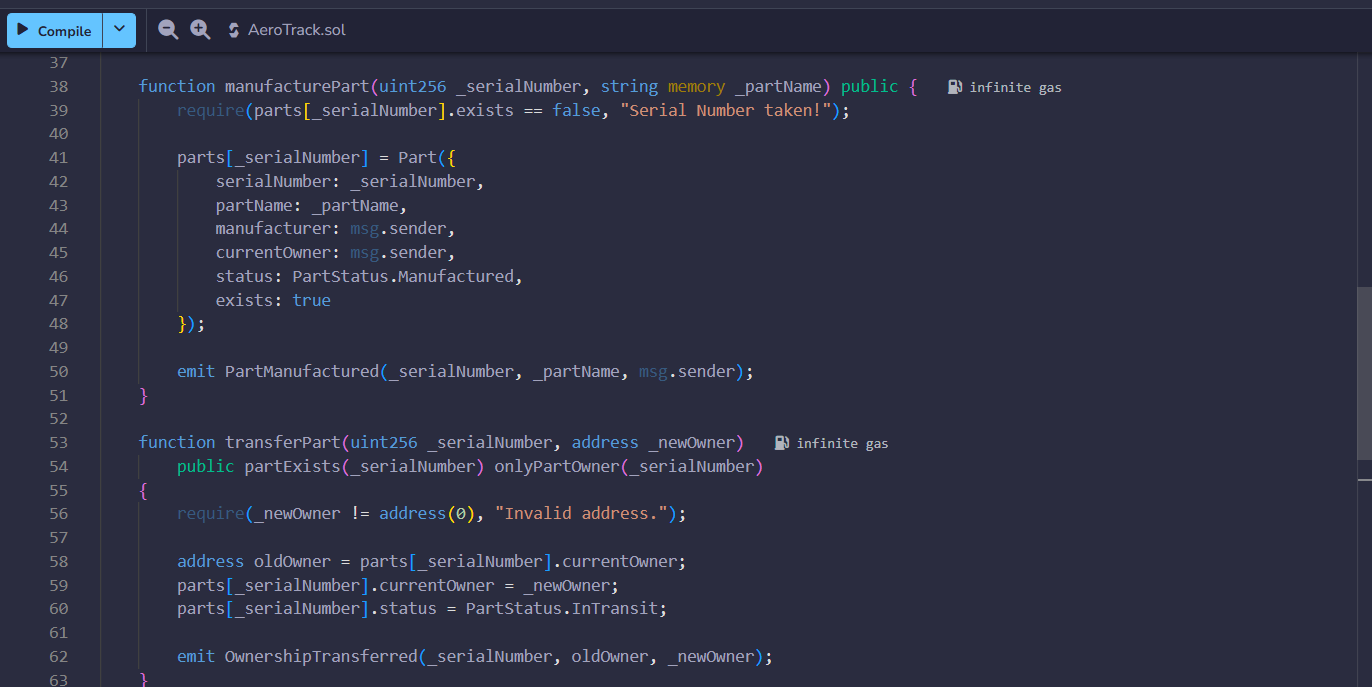
\includegraphics[width=0.85\textwidth]{../screens/step3-code.png}
    \caption{Core functions code in the Remix editor}
    \label{fig:step3-code}
\end{figure}

\begin{figure}[H]
    \centering
    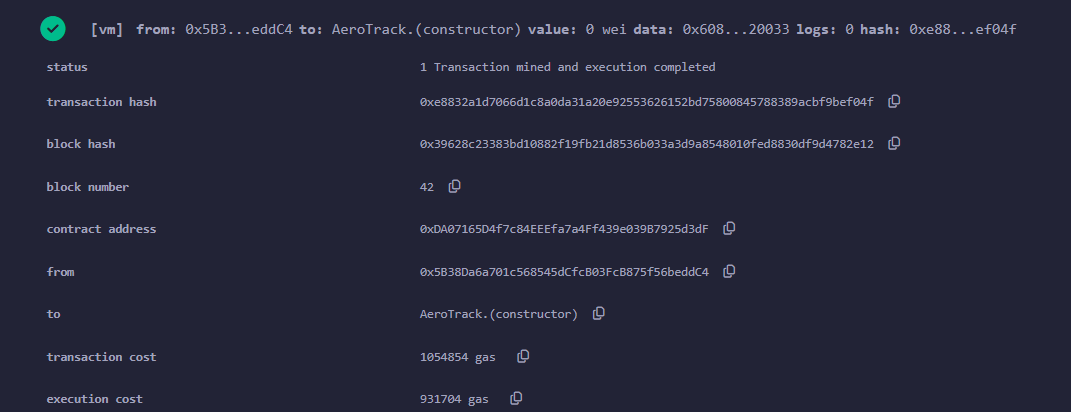
\includegraphics[width=0.85\textwidth]{../screens/step3-deploy-success.png}
    \caption{Successful deployment of the contract with core functions}
    \label{fig:step3-deploy}
\end{figure}

\begin{figure}[H]
    \centering
    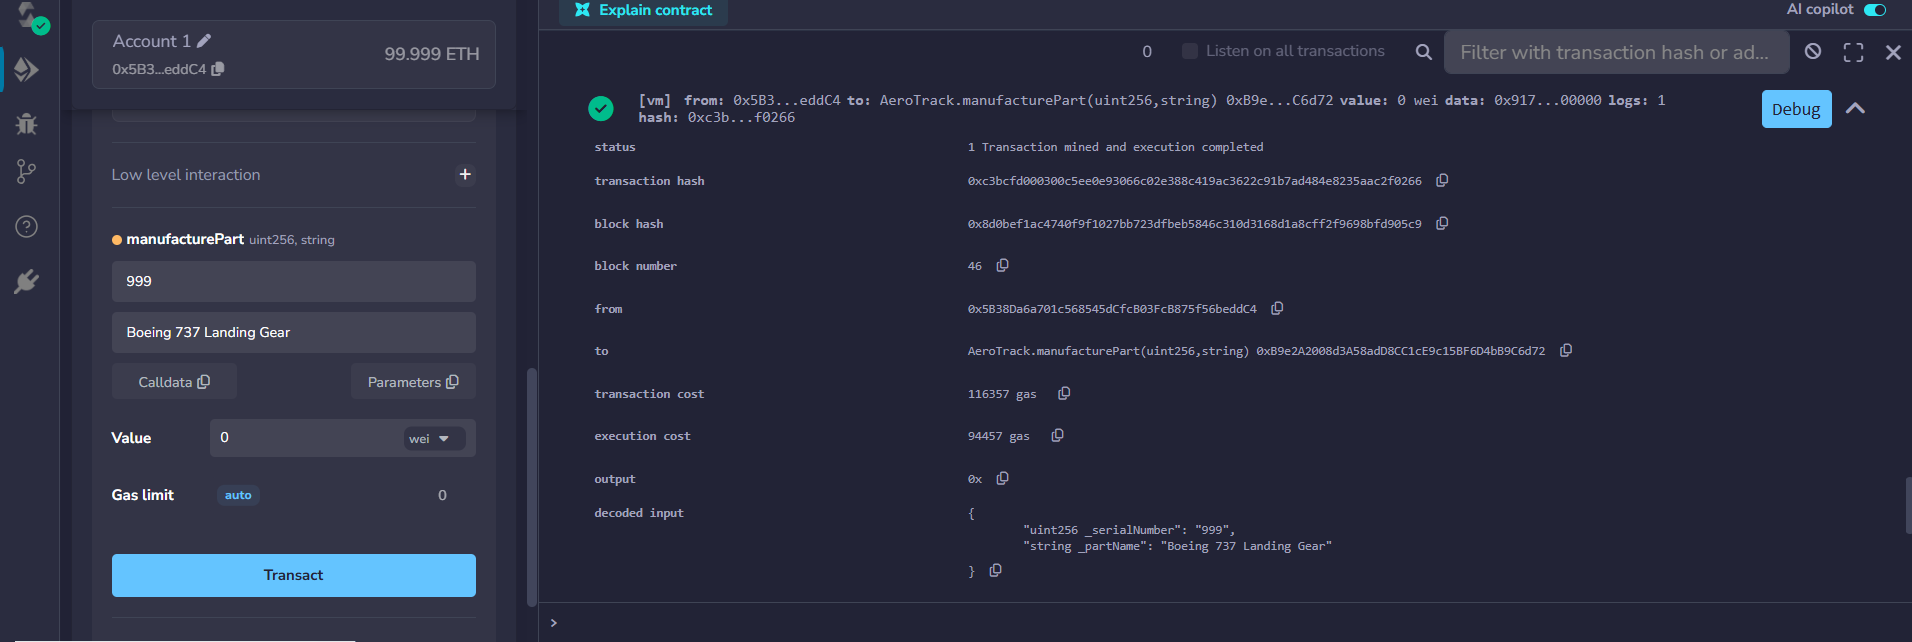
\includegraphics[width=0.85\textwidth]{../screens/step3-manufacturePart.png}
    \caption{Calling \texttt{manufacturePart} to register a new part (serial 999)}
    \label{fig:step3-manufacture}
\end{figure}

\begin{figure}[H]
    \centering
    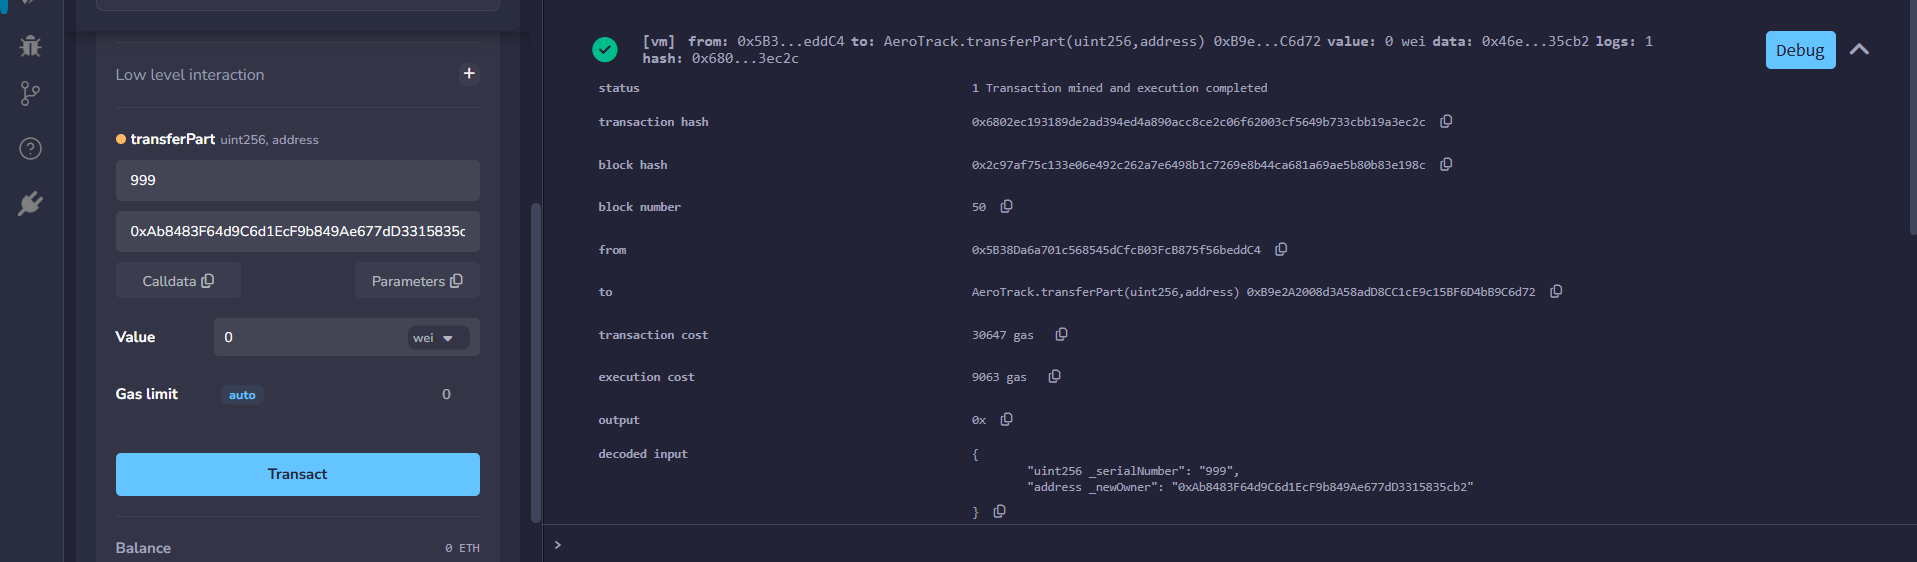
\includegraphics[width=0.85\textwidth]{../screens/step3-transferPart.png}
    \caption{Successful ownership transfer from manufacturer to airline}
    \label{fig:step3-transfer}
\end{figure}

\begin{figure}[H]
    \centering
    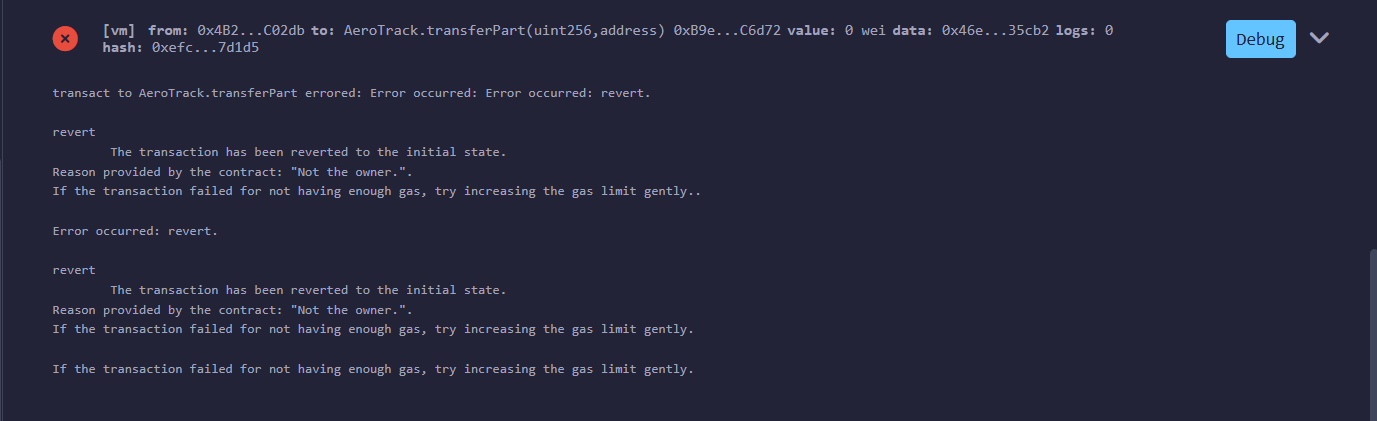
\includegraphics[width=0.85\textwidth]{../screens/step3-hack-fail.png}
    \caption{Security test: unauthorized transfer attempt reverts with ``Not the owner''}
    \label{fig:step3-hack}
\end{figure}

\subsection{Step 4: Events and Traceability}

Events provide a gas-efficient way to log historical data. They are written to transaction logs (not contract storage), making them approximately 10--100x cheaper.

\begin{lstlisting}[caption={Event declarations and maintenance function}]
event PartManufactured(uint256 indexed serialNumber,
                       string partName, address manufacturer);
event OwnershipTransferred(uint256 indexed serialNumber,
                           address oldOwner, address newOwner);
event MaintenanceLogged(uint256 indexed serialNumber,
                        address mechanic, string report);

function logMaintenance(uint256 _serialNumber,
                        string memory _report)
    public partExists(_serialNumber) onlyPartOwner(_serialNumber)
{
    emit MaintenanceLogged(_serialNumber, msg.sender, _report);
    parts[_serialNumber].status = PartStatus.Installed;
}
\end{lstlisting}

The \texttt{indexed} keyword allows external applications to efficiently filter events by serial number.

Figures~\ref{fig:step4-code} to~\ref{fig:step4-maintenance} demonstrate the events in action.

\begin{figure}[H]
    \centering
    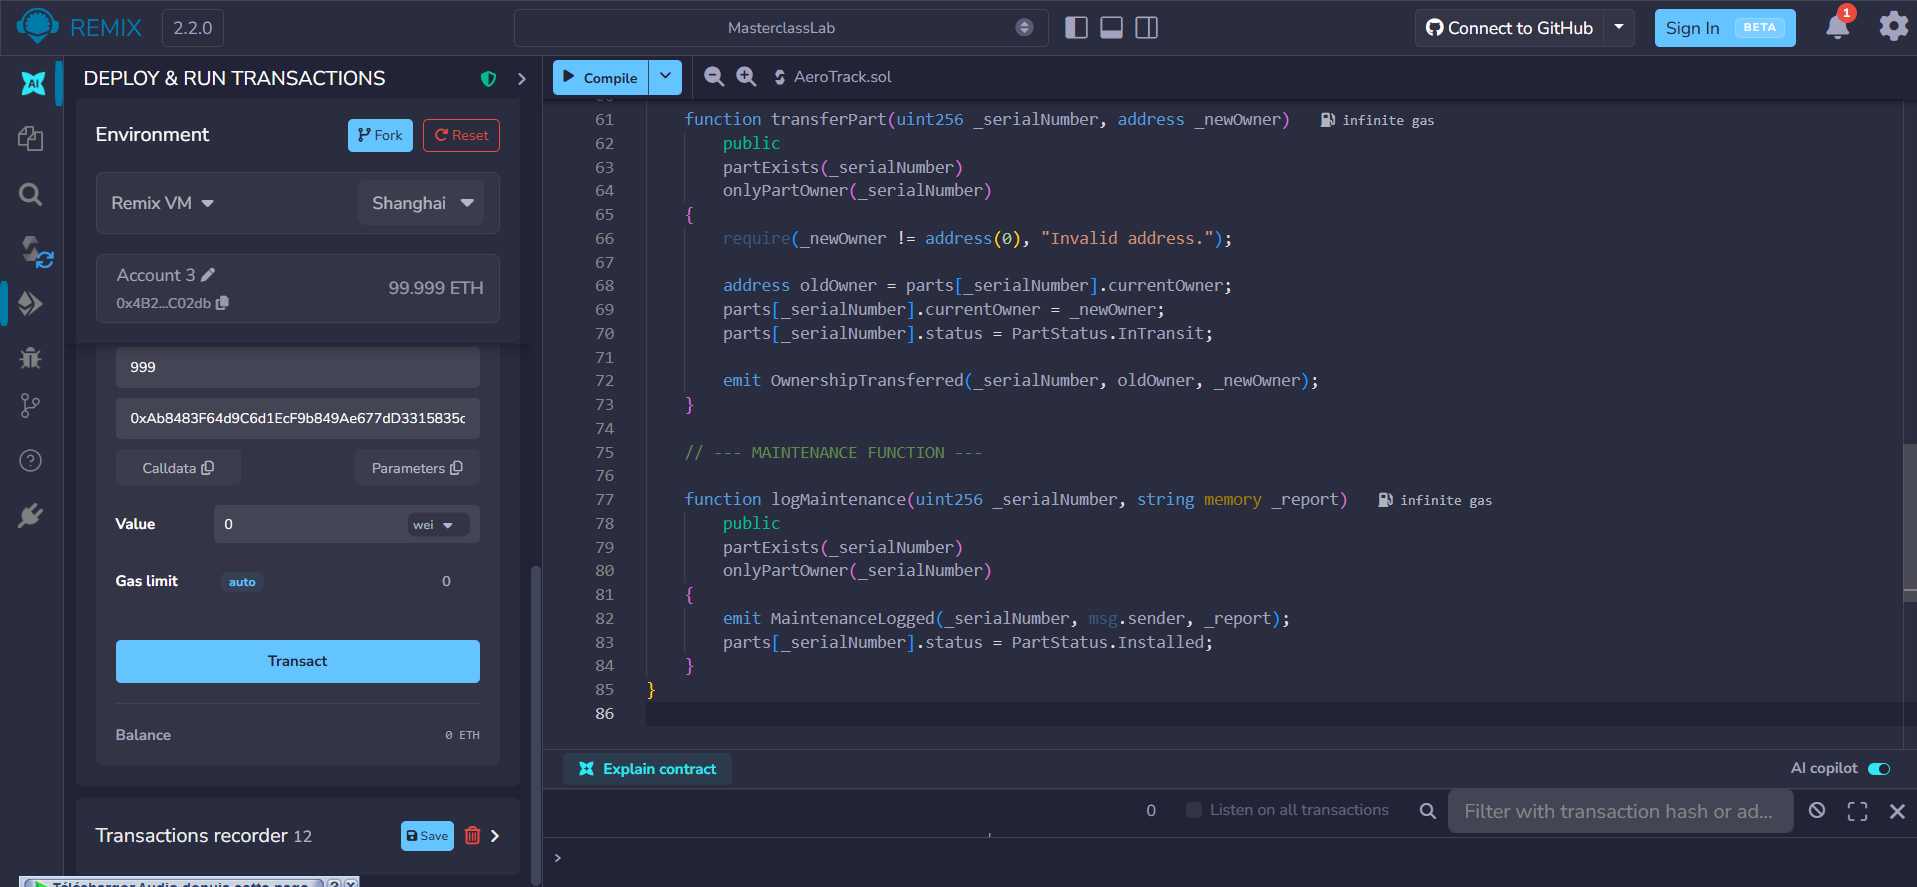
\includegraphics[width=0.85\textwidth]{../screens/step4-code.png}
    \caption{Contract code with event declarations and \texttt{logMaintenance} function}
    \label{fig:step4-code}
\end{figure}

\begin{figure}[H]
    \centering
    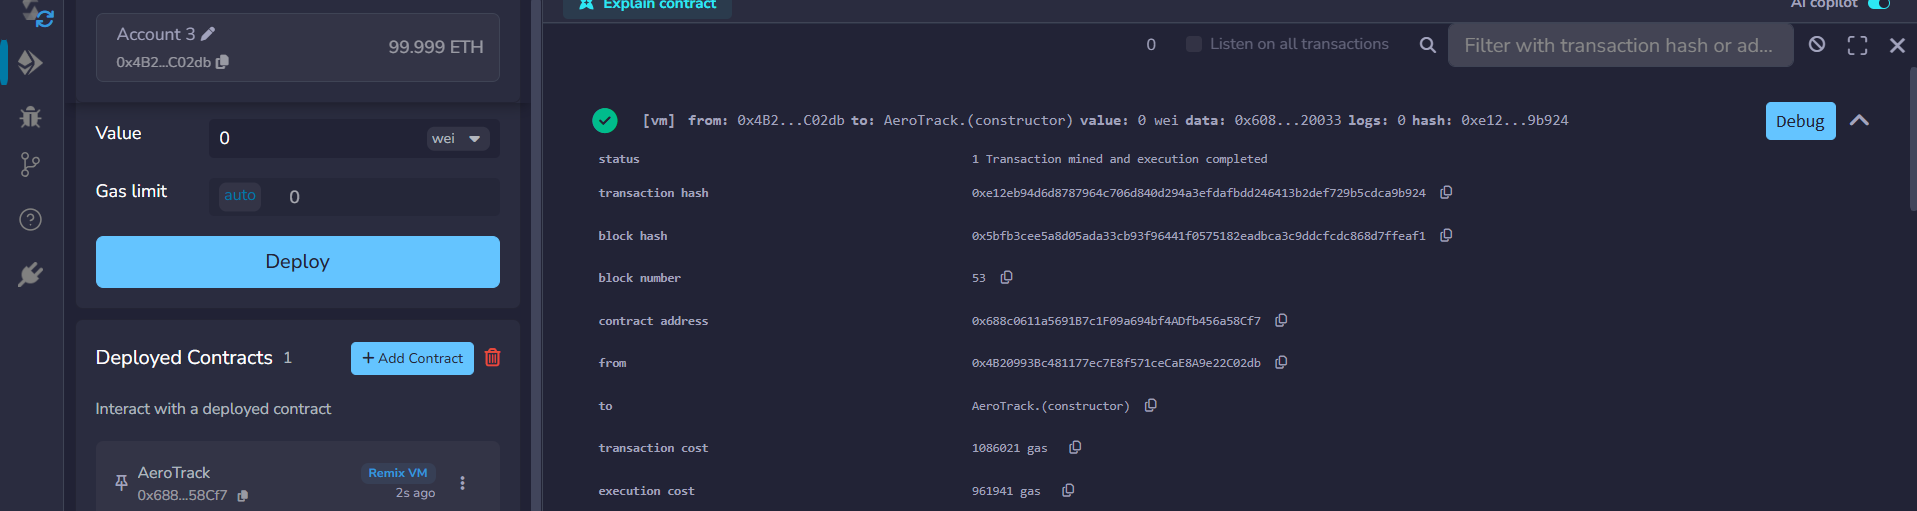
\includegraphics[width=0.85\textwidth]{../screens/step4-deploy-success.png}
    \caption{Successful deployment of the contract with events}
    \label{fig:step4-deploy}
\end{figure}

\begin{figure}[H]
    \centering
    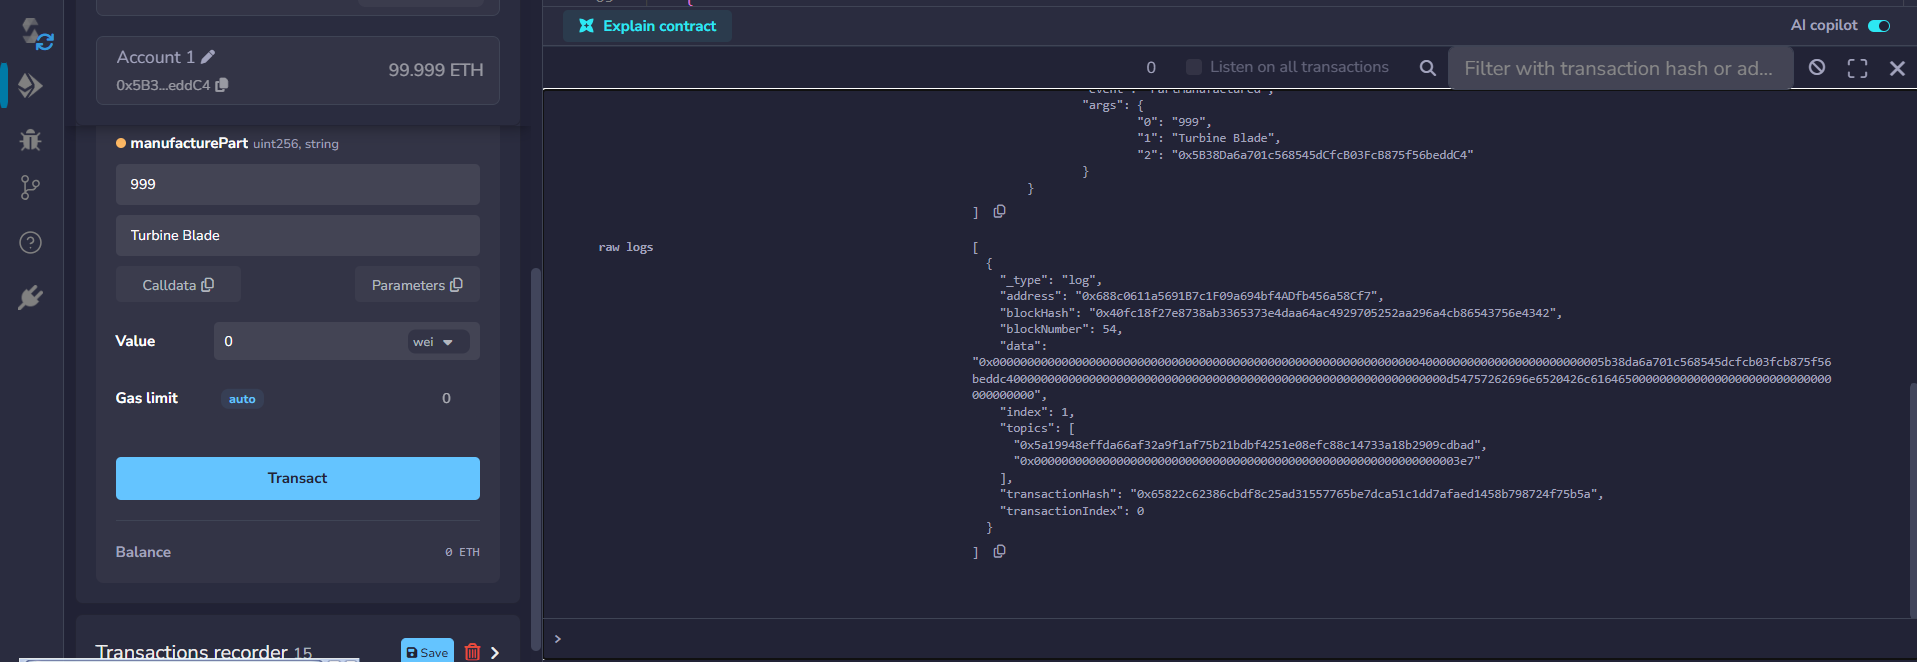
\includegraphics[width=0.85\textwidth]{../screens/step4-manufacture-event.png}
    \caption{Transaction logs showing the \texttt{PartManufactured} event}
    \label{fig:step4-manufacture}
\end{figure}

\begin{figure}[H]
    \centering
    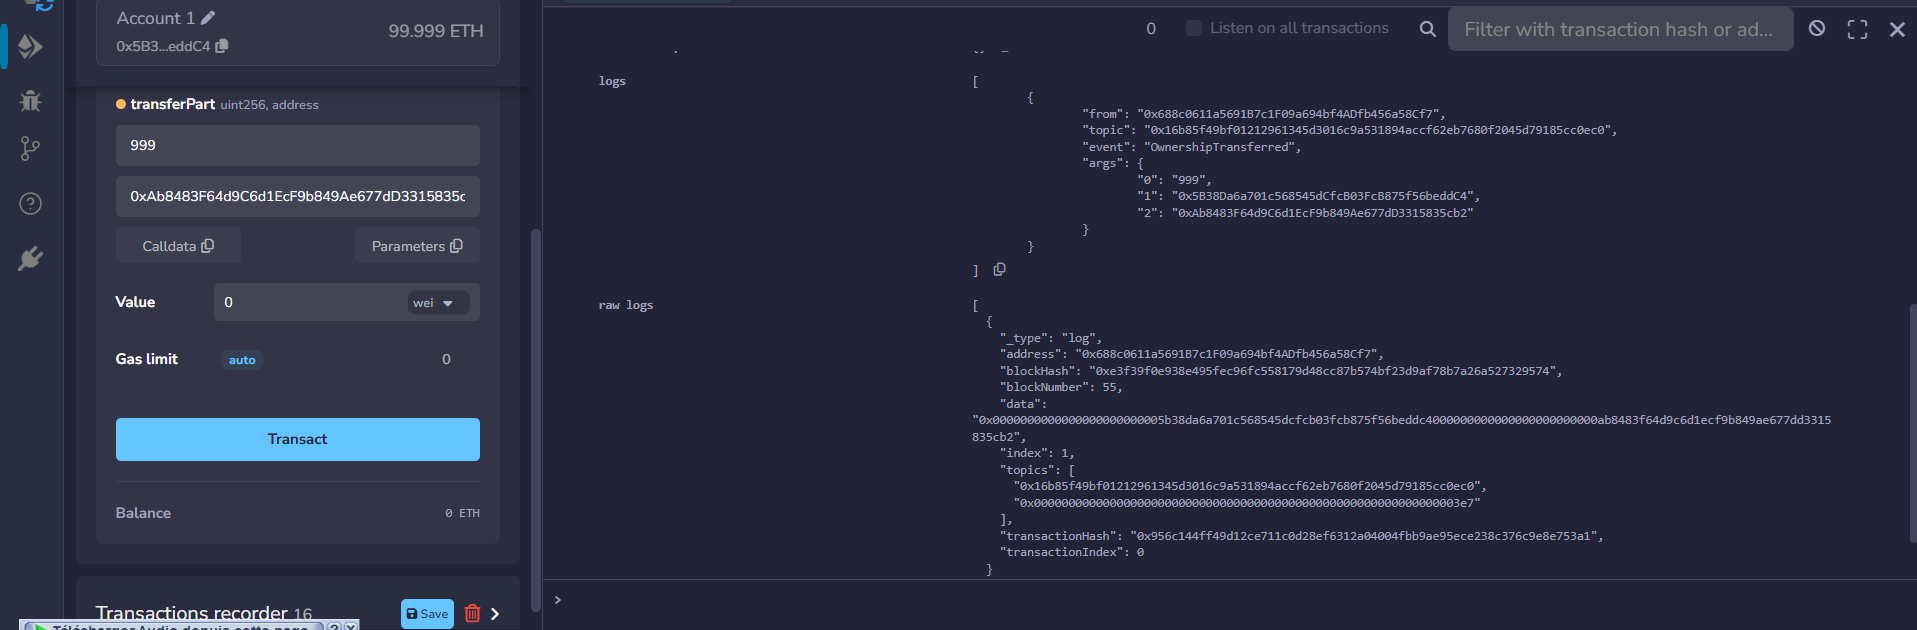
\includegraphics[width=0.85\textwidth]{../screens/step4-transfer-event.png}
    \caption{Transaction logs showing the \texttt{OwnershipTransferred} event}
    \label{fig:step4-transfer}
\end{figure}

\begin{figure}[H]
    \centering
    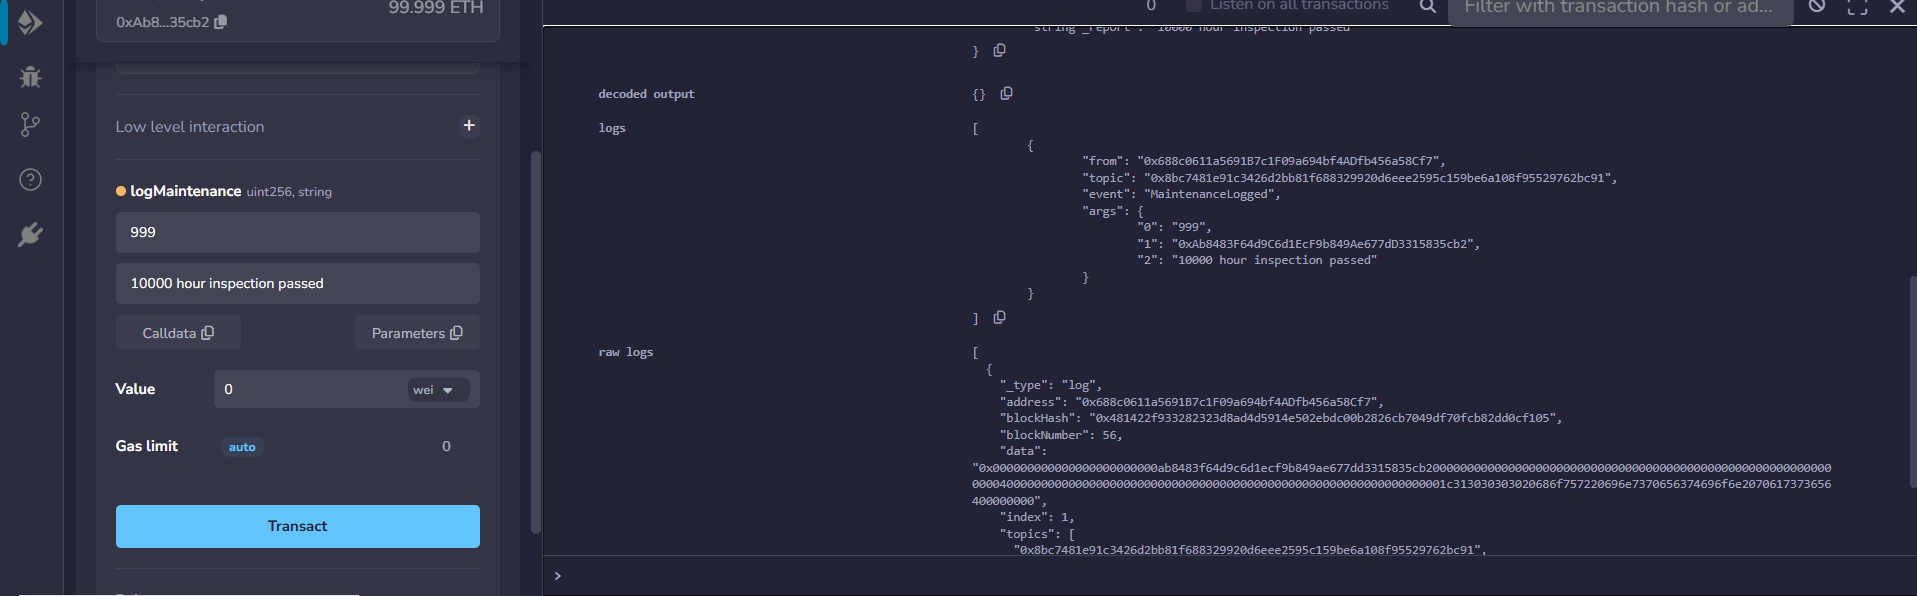
\includegraphics[width=0.85\textwidth]{../screens/step4-logMaintenance.png}
    \caption{Calling \texttt{logMaintenance} -- event emitted with maintenance report}
    \label{fig:step4-maintenance}
\end{figure}

% ============================================================
\subsection{Step 5: Enhancement -- Certified Manufacturer Registry}
% ============================================================

To address the \textbf{Decentralized Identifiers (DIDs)} topic from the lab's future research section, we implemented a manufacturer certification system. The \texttt{regulatoryAuthority} (FAA/EASA) maintains a registry of approved manufacturers. Only certified addresses can call \texttt{manufacturePart}.

\begin{lstlisting}[caption={Manufacturer certification system}]
mapping(address => bool) public certifiedManufacturers;

modifier onlyAuthority() {
    require(msg.sender == regulatoryAuthority, "Not the authority.");
    _;
}

modifier onlyCertified() {
    require(certifiedManufacturers[msg.sender],
            "Not a certified manufacturer.");
    _;
}

function certifyManufacturer(address _manufacturer)
    public onlyAuthority {
    certifiedManufacturers[_manufacturer] = true;
    emit ManufacturerCertified(_manufacturer);
}

function revokeManufacturer(address _manufacturer)
    public onlyAuthority {
    certifiedManufacturers[_manufacturer] = false;
    emit ManufacturerRevoked(_manufacturer);
}
\end{lstlisting}

The \texttt{manufacturePart} function now includes the \texttt{onlyCertified} modifier, preventing uncertified addresses from registering parts.

\begin{figure}[H]
    \centering
    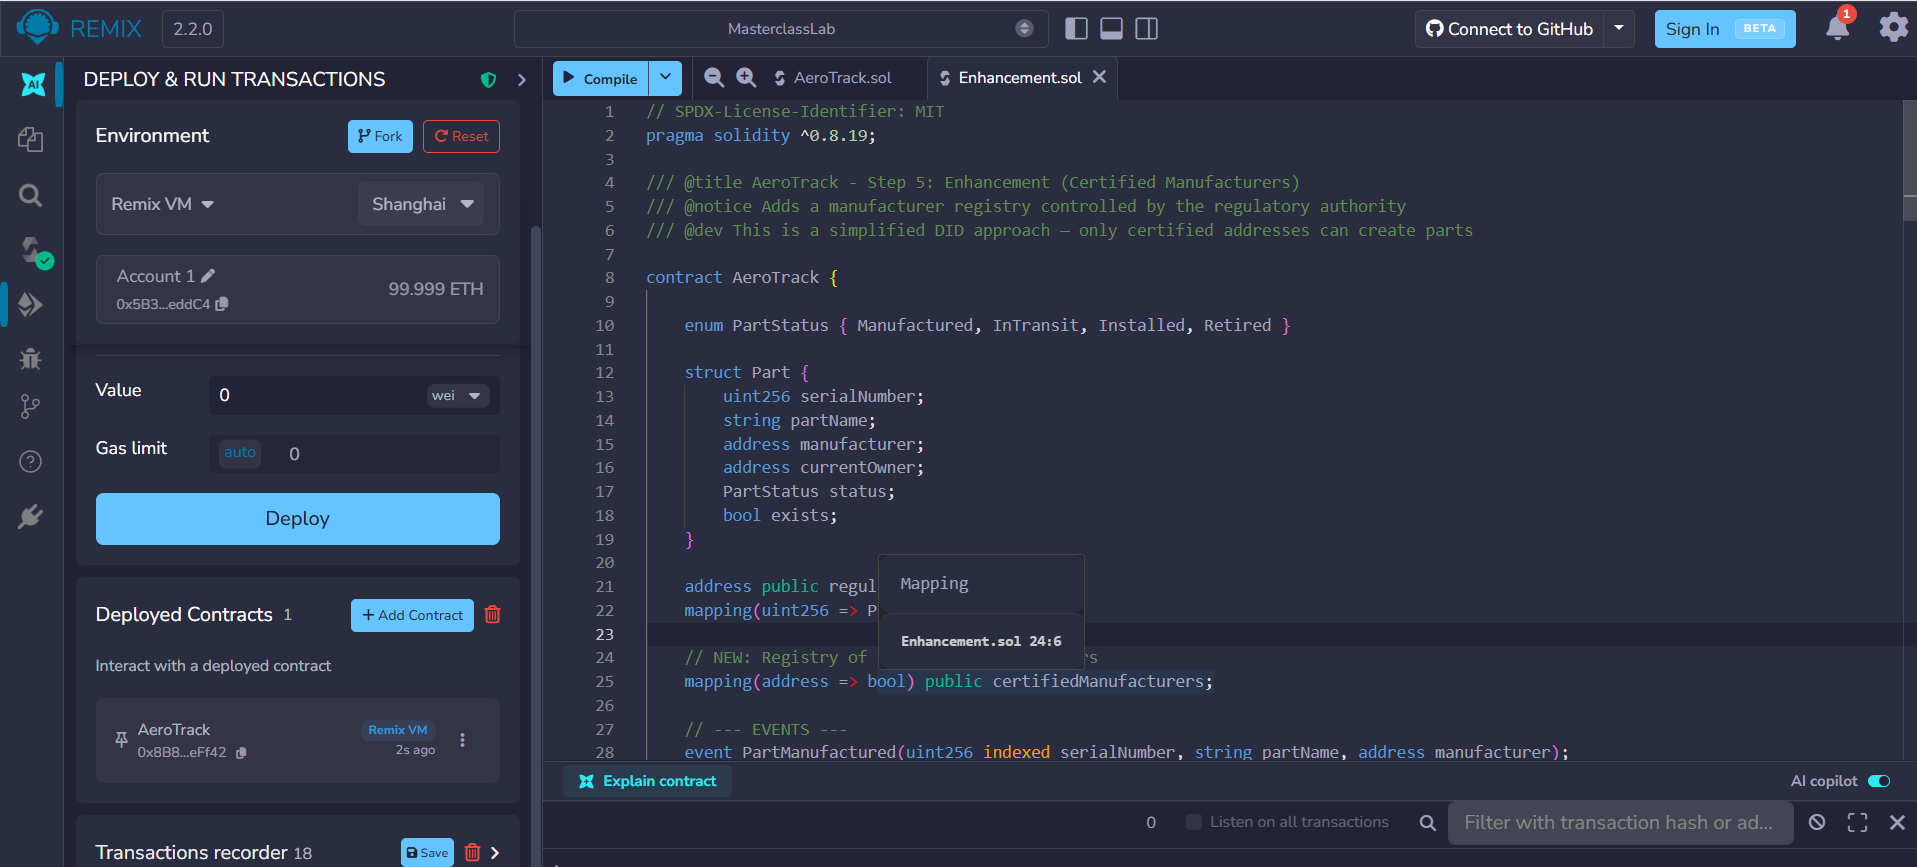
\includegraphics[width=0.85\textwidth]{../screens/step5-code.png}
    \caption{Enhanced contract with manufacturer certification system}
    \label{fig:step5-code}
\end{figure}

\begin{figure}[H]
    \centering
    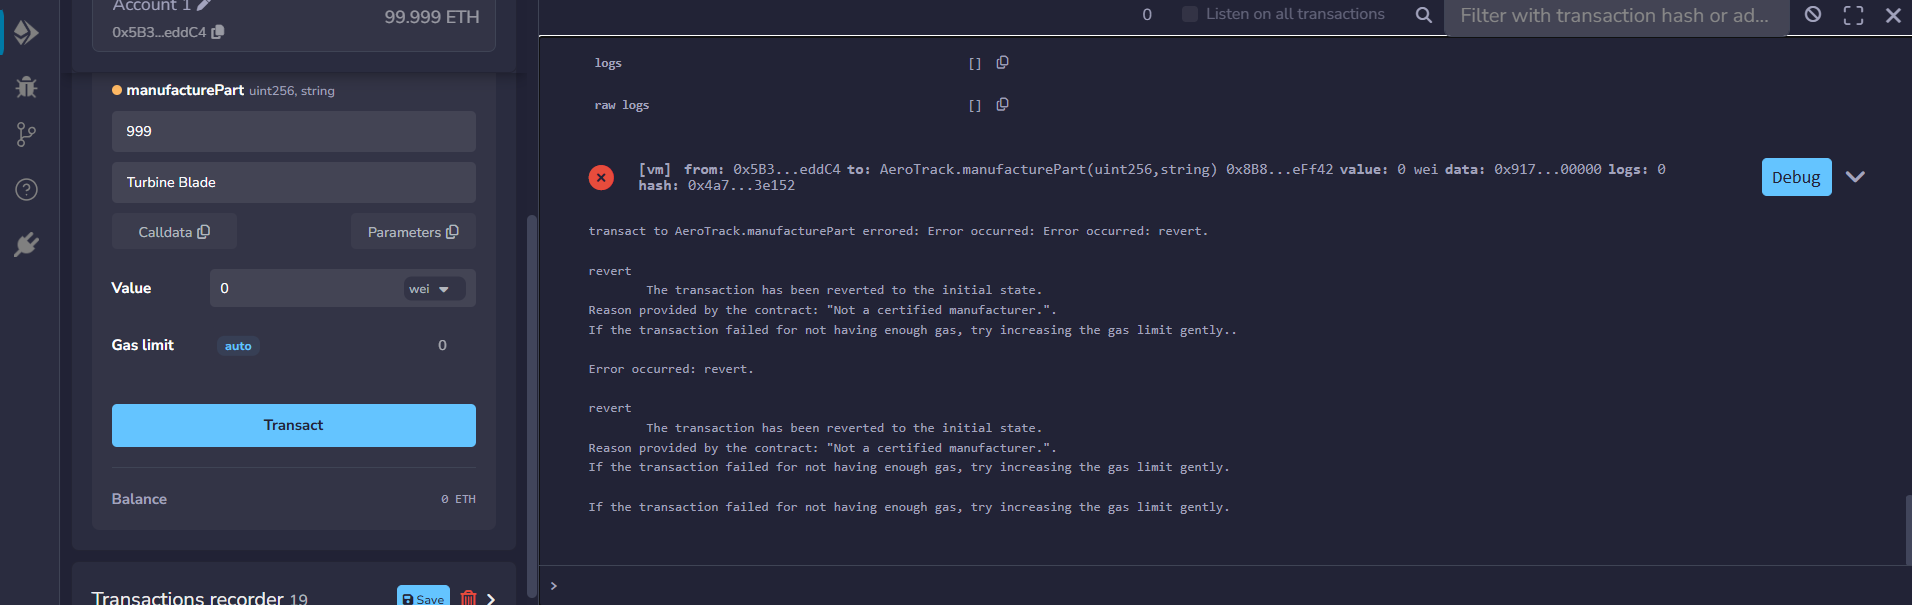
\includegraphics[width=0.85\textwidth]{../screens/step5-fail-uncertified.png}
    \caption{Manufacturing attempt fails without certification}
    \label{fig:step5-fail}
\end{figure}

\begin{figure}[H]
    \centering
    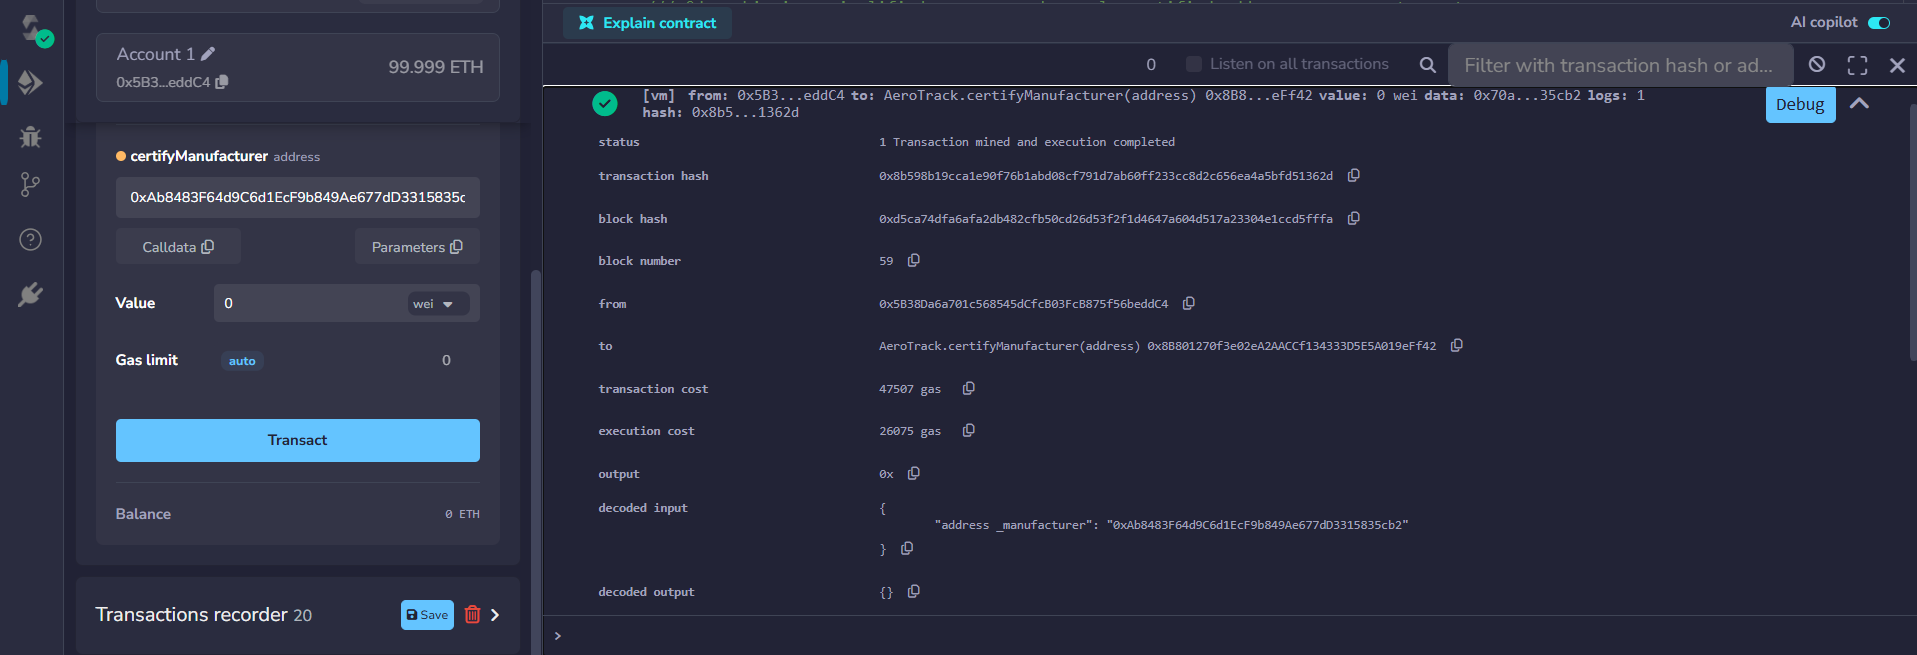
\includegraphics[width=0.85\textwidth]{../screens/step5-certifyManufacturer.png}
    \caption{Authority certifies Account 2 as a manufacturer}
    \label{fig:step5-certify}
\end{figure}

\begin{figure}[H]
    \centering
    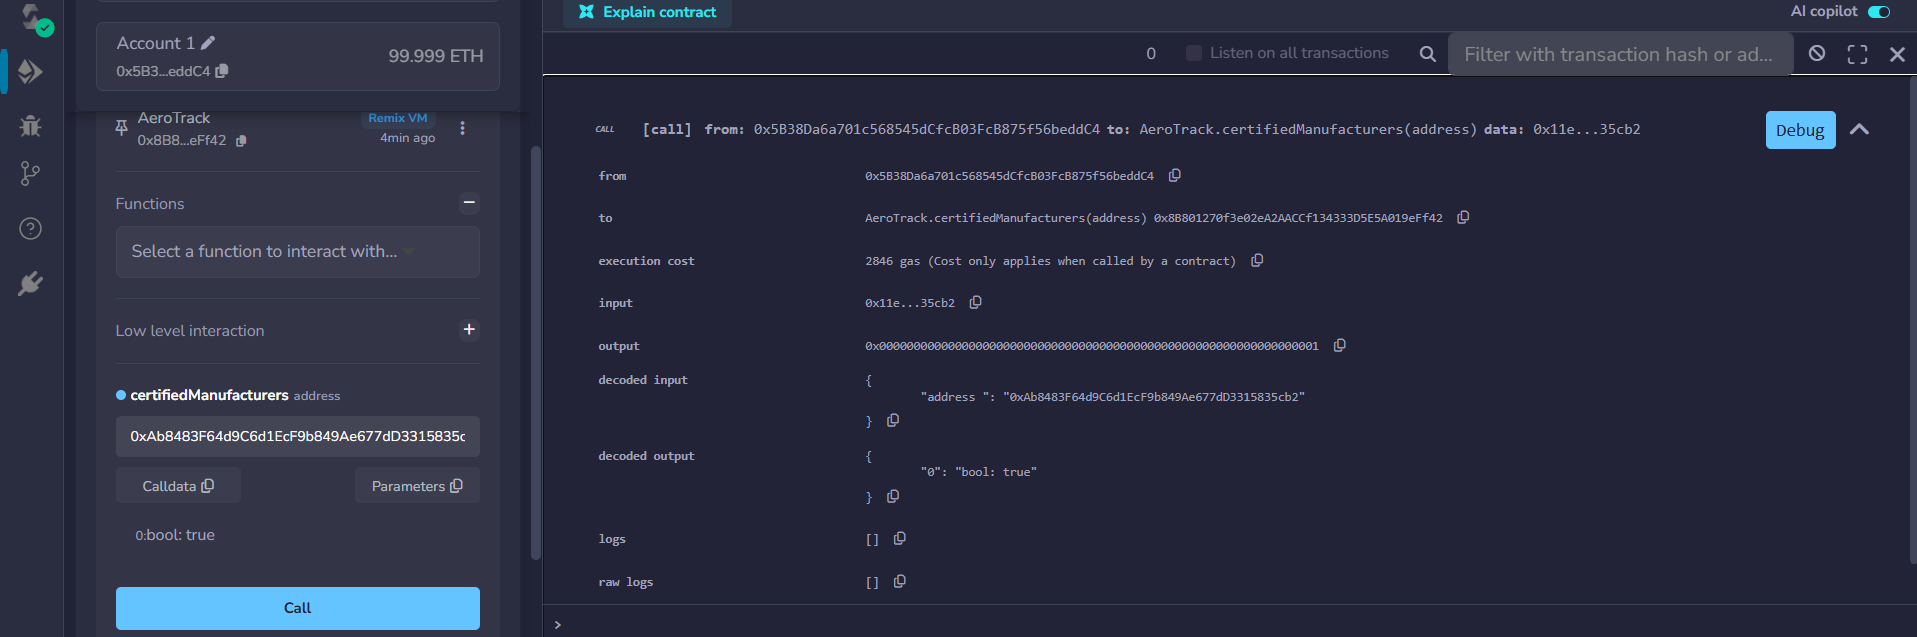
\includegraphics[width=0.85\textwidth]{../screens/step5-certifiedManufacturers-check.png}
    \caption{Verifying certification status returns \texttt{true}}
    \label{fig:step5-check}
\end{figure}

\begin{figure}[H]
    \centering
    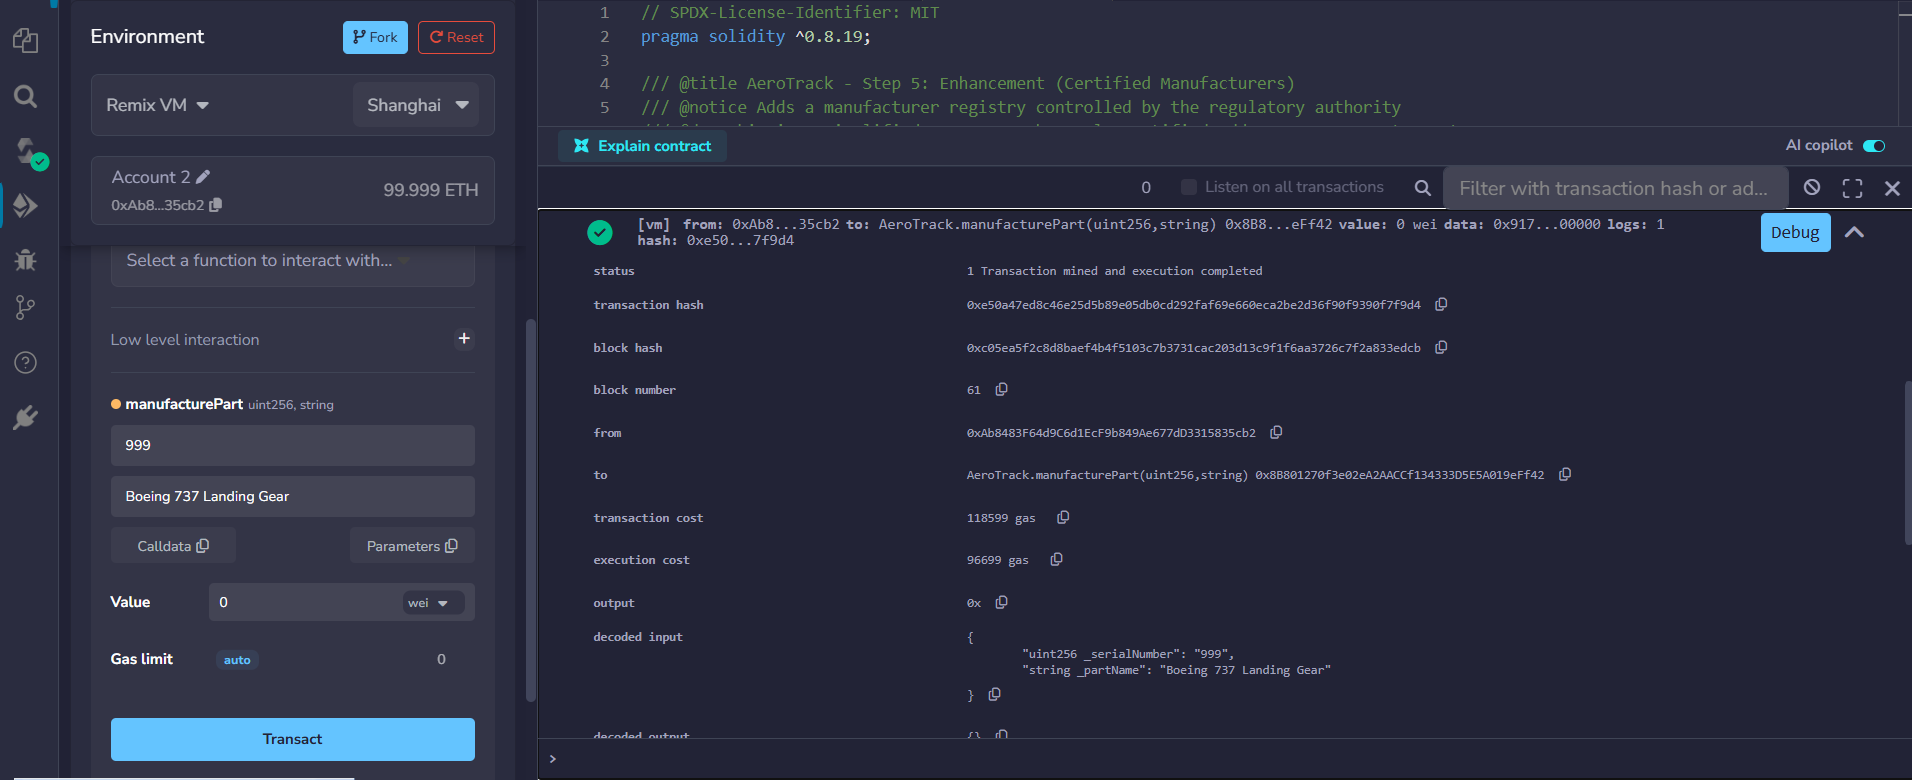
\includegraphics[width=0.85\textwidth]{../screens/step5-manufacture-account2-success.png}
    \caption{Certified Account 2 successfully manufactures a part}
    \label{fig:step5-success}
\end{figure}

\begin{figure}[H]
    \centering
    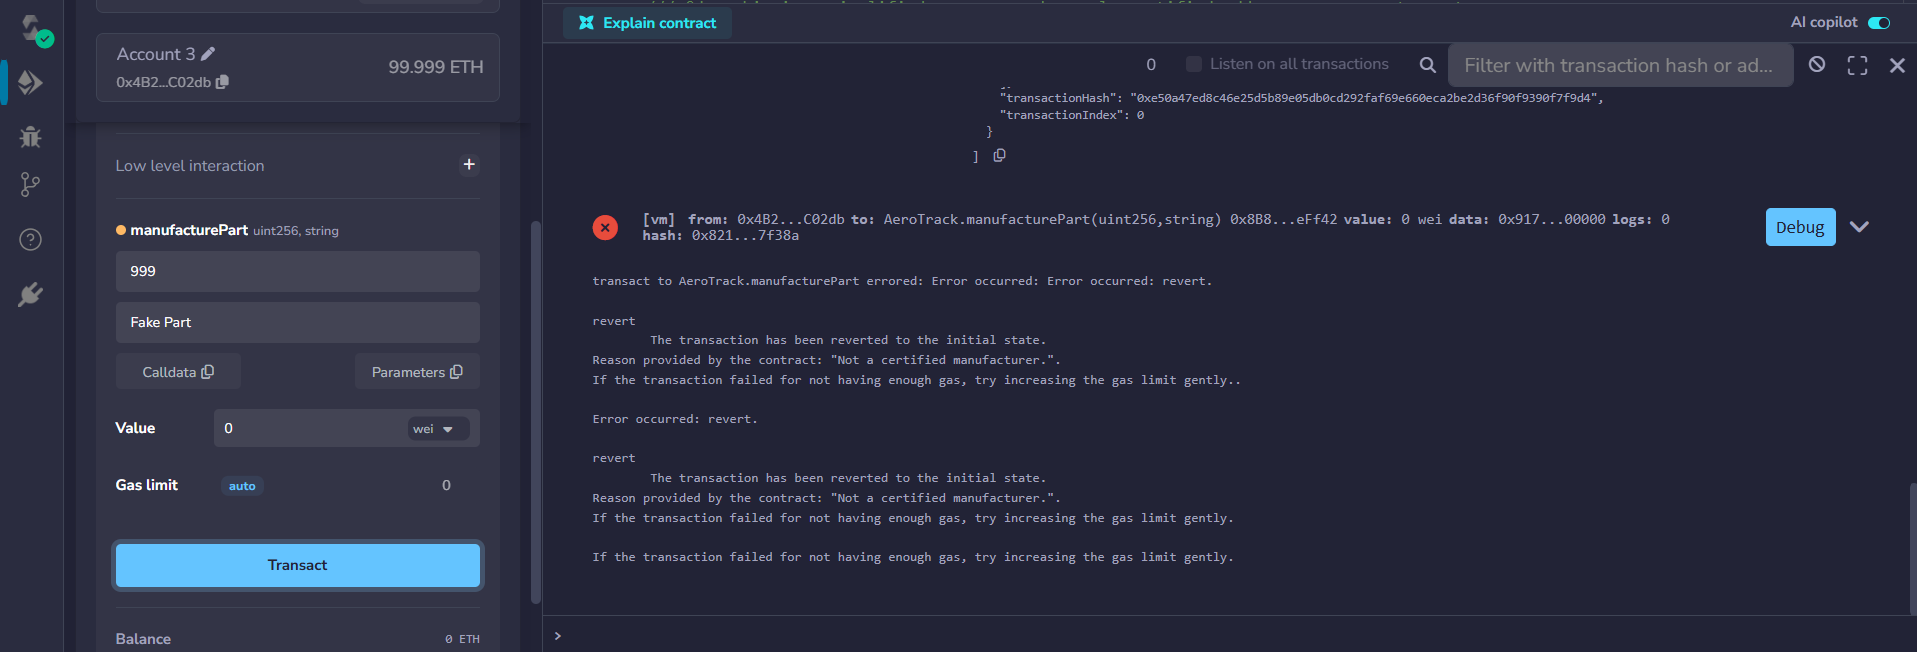
\includegraphics[width=0.85\textwidth]{../screens/step5-fail-account3.png}
    \caption{Uncertified Account 3 fails to manufacture}
    \label{fig:step5-fail3}
\end{figure}

\begin{figure}[H]
    \centering
    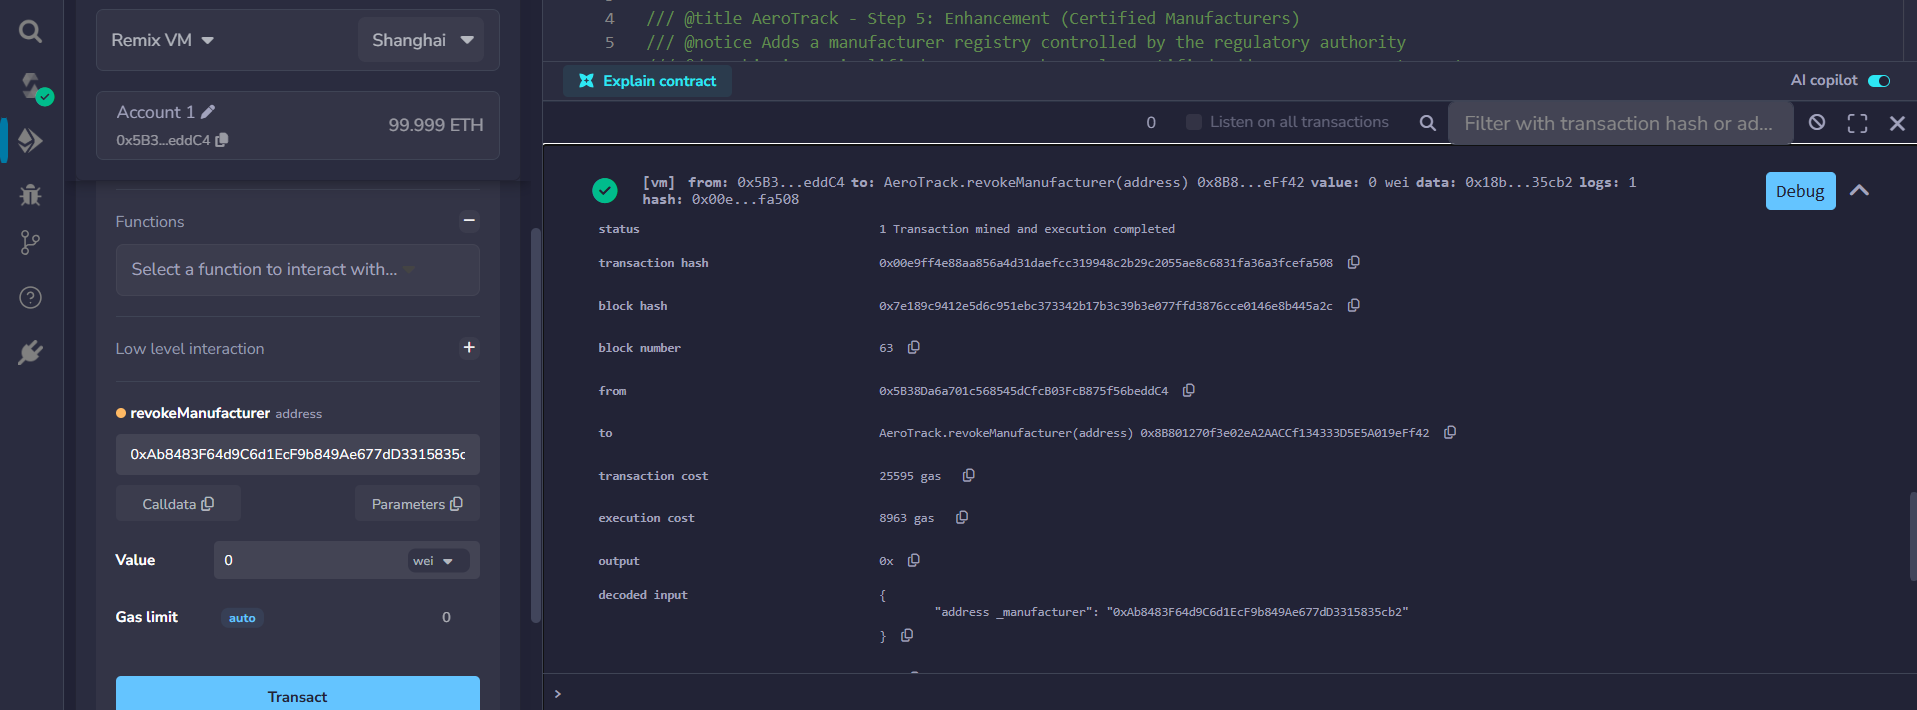
\includegraphics[width=0.85\textwidth]{../screens/step5-revokeManufacturer.png}
    \caption{Authority revokes Account 2's certification}
    \label{fig:step5-revoke}
\end{figure}

\begin{figure}[H]
    \centering
    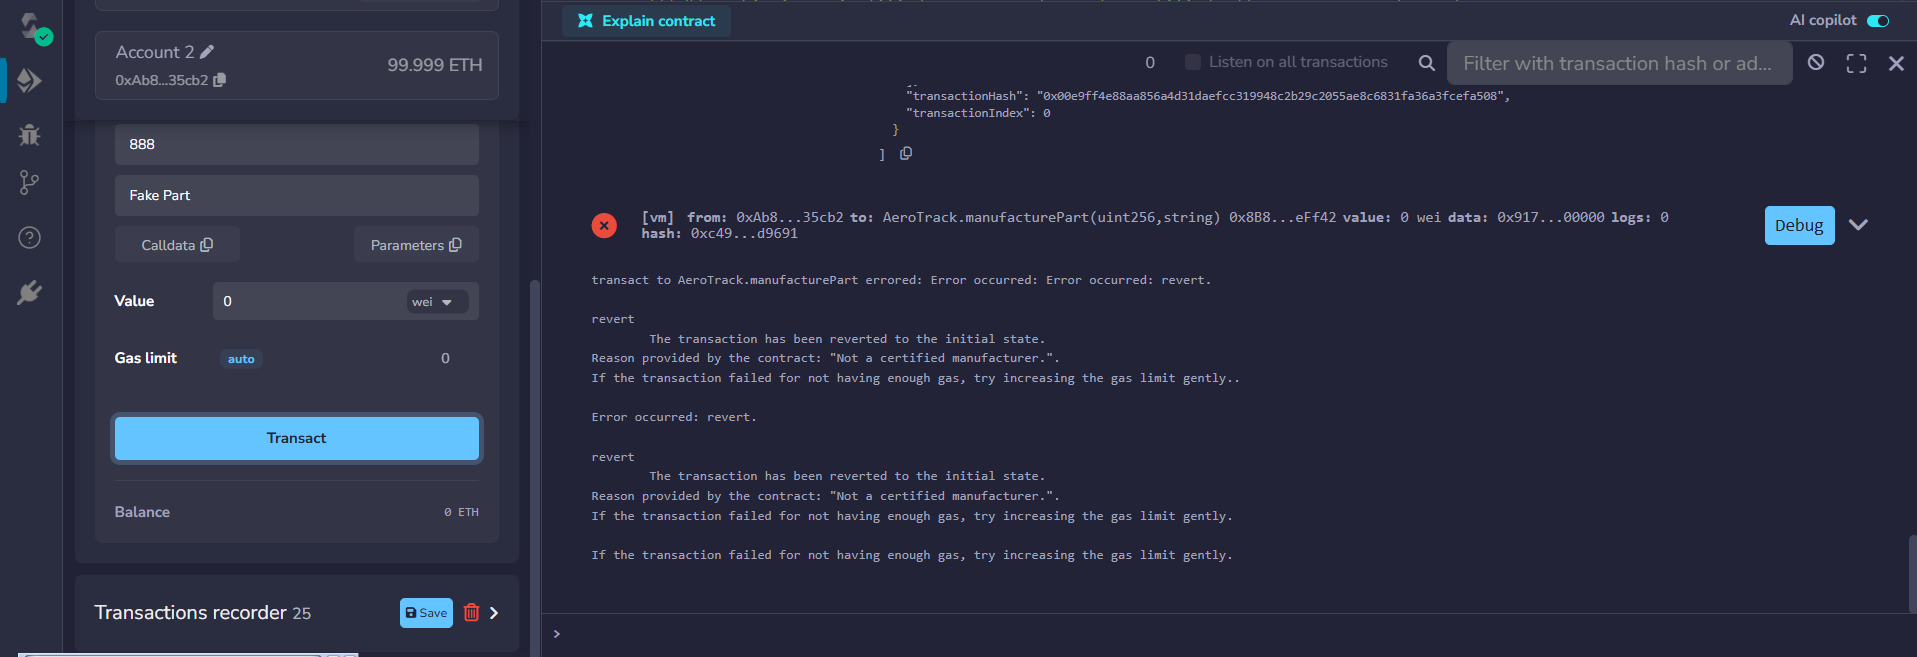
\includegraphics[width=0.85\textwidth]{../screens/step5-fail-after-revoke.png}
    \caption{Account 2 fails to manufacture after revocation}
    \label{fig:step5-revoked}
\end{figure}

% ============================================================
\subsection{Step 6: Decentralized Identifiers (DIDs)}
% ============================================================

To fully address the DID research question, we extended the certification system with \textbf{on-chain identity storage}. Instead of a simple boolean, the authority now registers a manufacturer's full identity: company name, country, and official certification number.

\begin{lstlisting}[caption={ManufacturerIdentity struct (DID)}]
struct ManufacturerIdentity {
    string name;              // e.g., "Boeing"
    string country;           // e.g., "USA"
    string certificationId;   // e.g., "FAA-2024-001"
    bool isActive;
    uint256 registeredAt;     // Block timestamp
}

mapping(address => ManufacturerIdentity)
    public manufacturerIdentities;
\end{lstlisting}

The \texttt{registerManufacturer} function stores the full identity and certifies the address simultaneously:

\begin{lstlisting}[caption={DID registration function}]
function registerManufacturer(
    address _manufacturer,
    string memory _name,
    string memory _country,
    string memory _certificationId
) public onlyAuthority {
    manufacturerIdentities[_manufacturer] = ManufacturerIdentity({
        name: _name,
        country: _country,
        certificationId: _certificationId,
        isActive: true,
        registeredAt: block.timestamp
    });
    certifiedManufacturers[_manufacturer] = true;
    emit ManufacturerRegistered(_manufacturer, _name, _certificationId);
}
\end{lstlisting}

This answers the lab's research question: anyone can query \texttt{manufacturerIdentities[address]} to cryptographically verify that an address belongs to a specific company.

\begin{figure}[H]
    \centering
    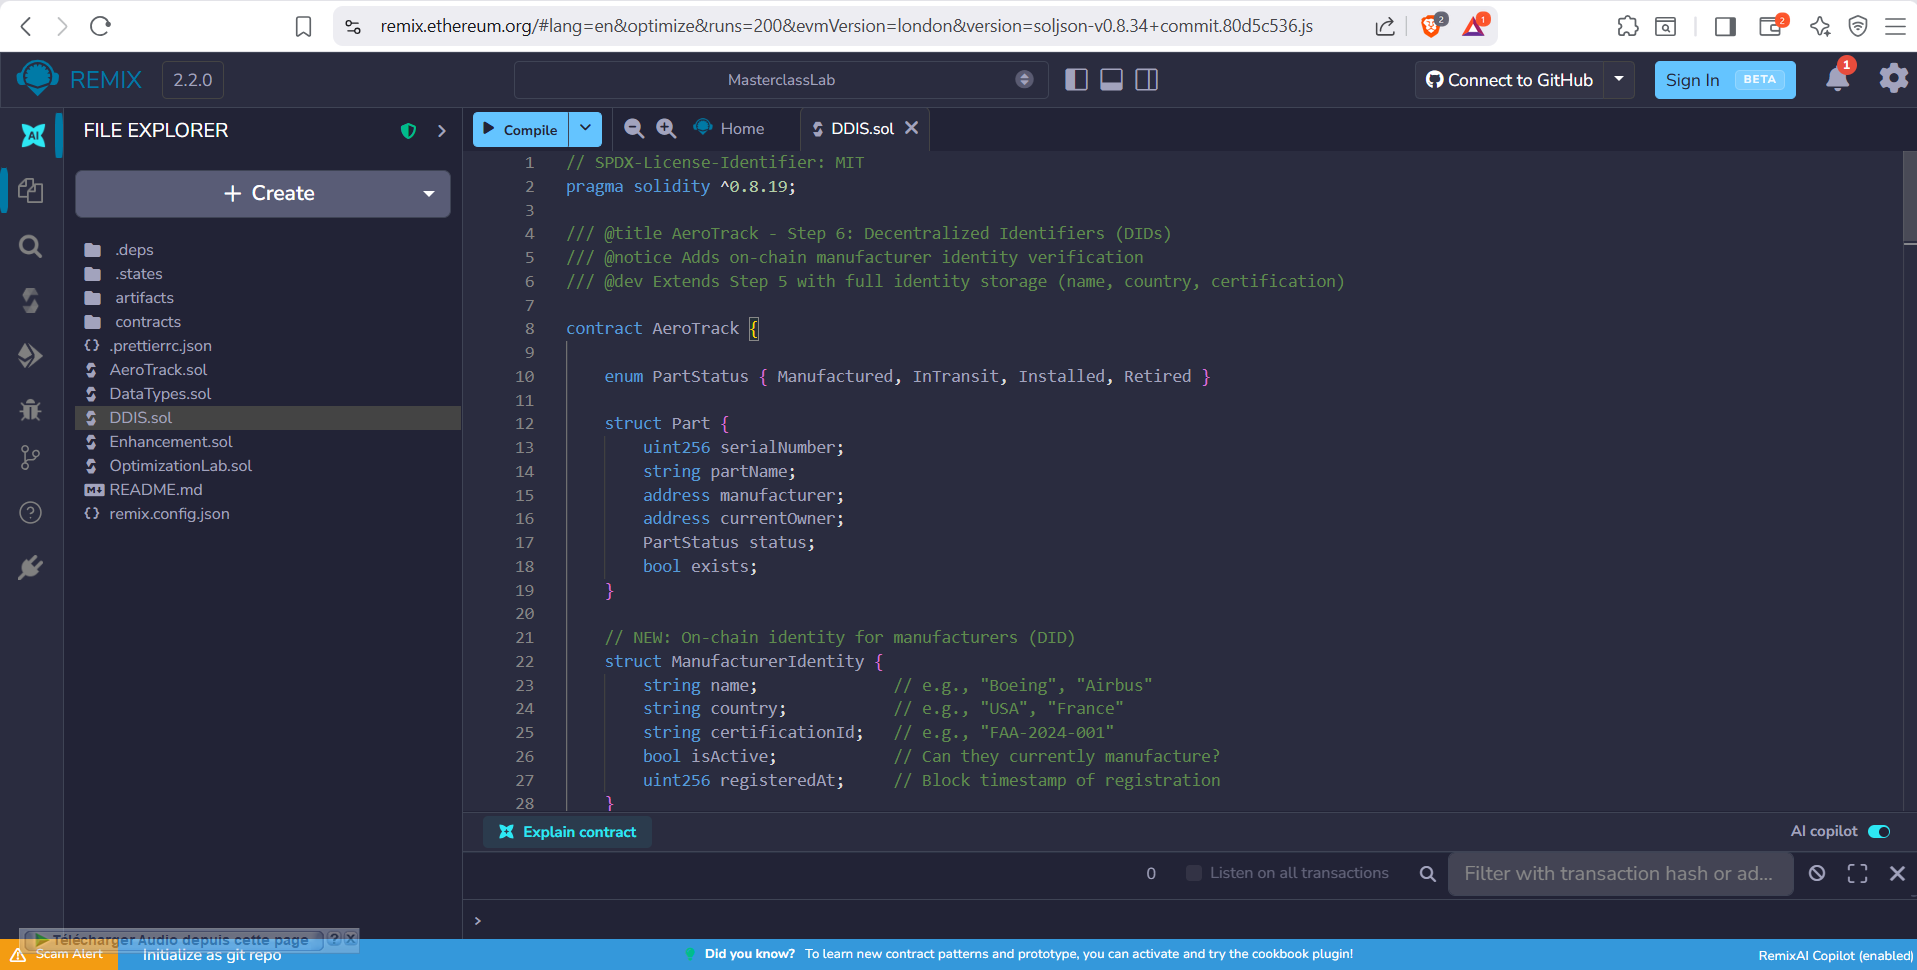
\includegraphics[width=0.85\textwidth]{../screens/step6-code.png}
    \caption{DID-enhanced contract code in Remix}
    \label{fig:step6-code}
\end{figure}

\begin{figure}[H]
    \centering
    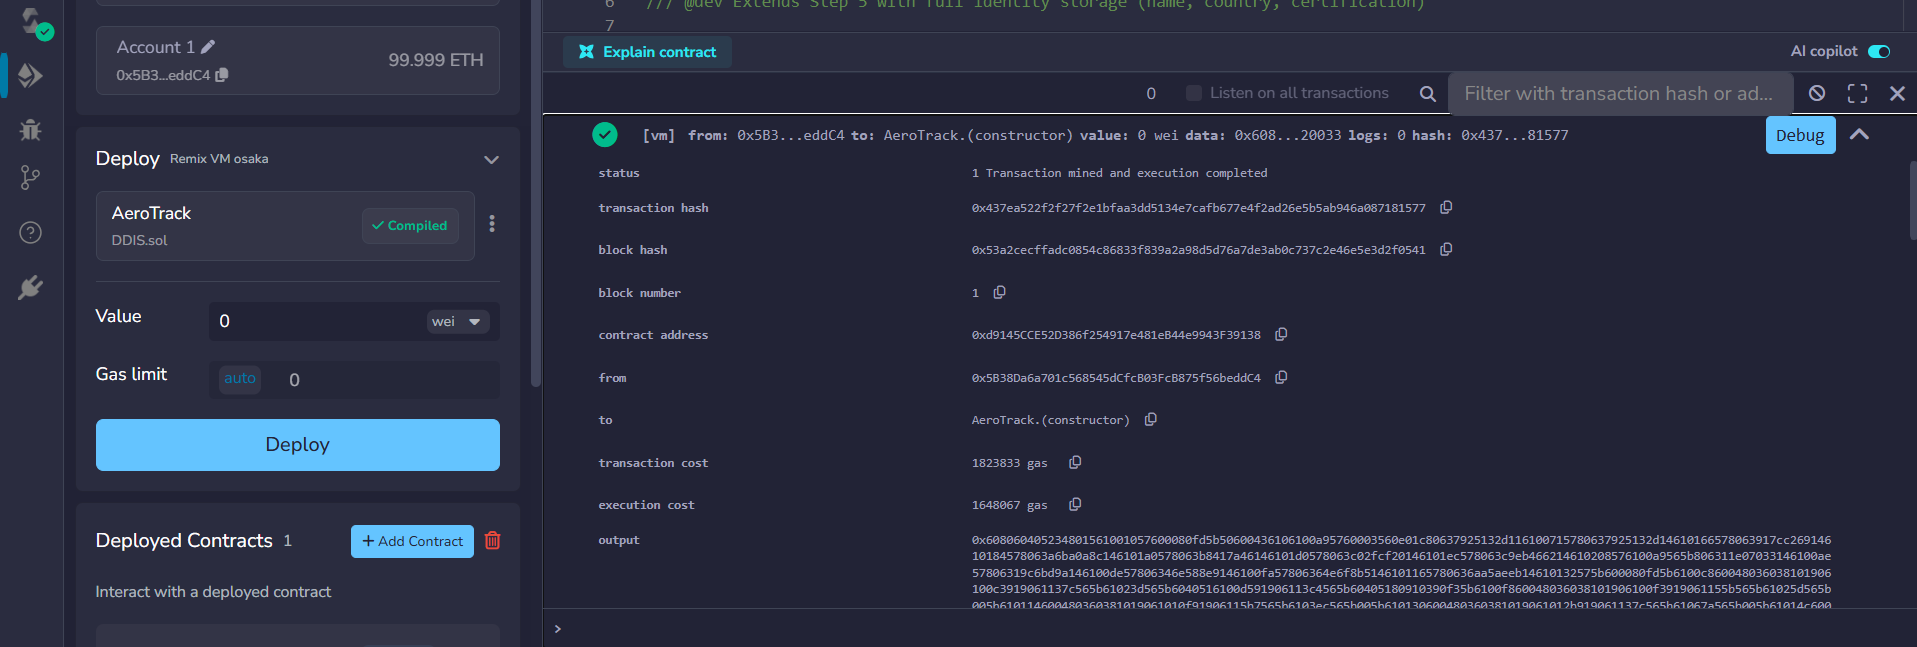
\includegraphics[width=0.85\textwidth]{../screens/step6-deploy-success.png}
    \caption{Successful deployment of the DID-enhanced contract}
    \label{fig:step6-deploy}
\end{figure}

\begin{figure}[H]
    \centering
    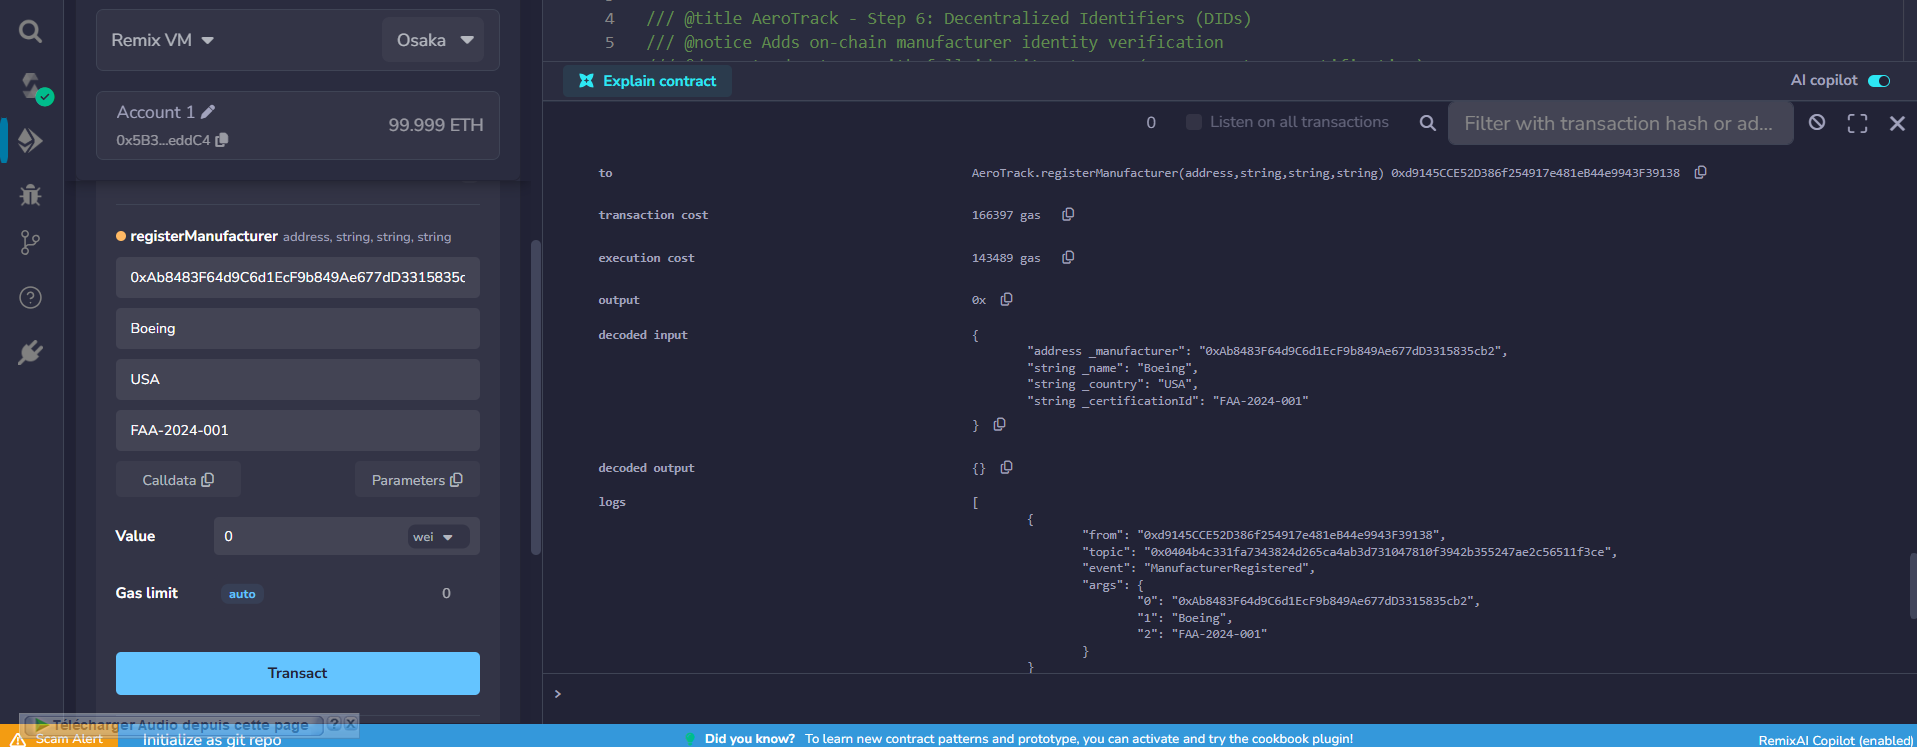
\includegraphics[width=0.85\textwidth]{../screens/step6-registerManufacturer.png}
    \caption{Authority registers Boeing with full identity (name, country, cert ID)}
    \label{fig:step6-register}
\end{figure}

\begin{figure}[H]
    \centering
    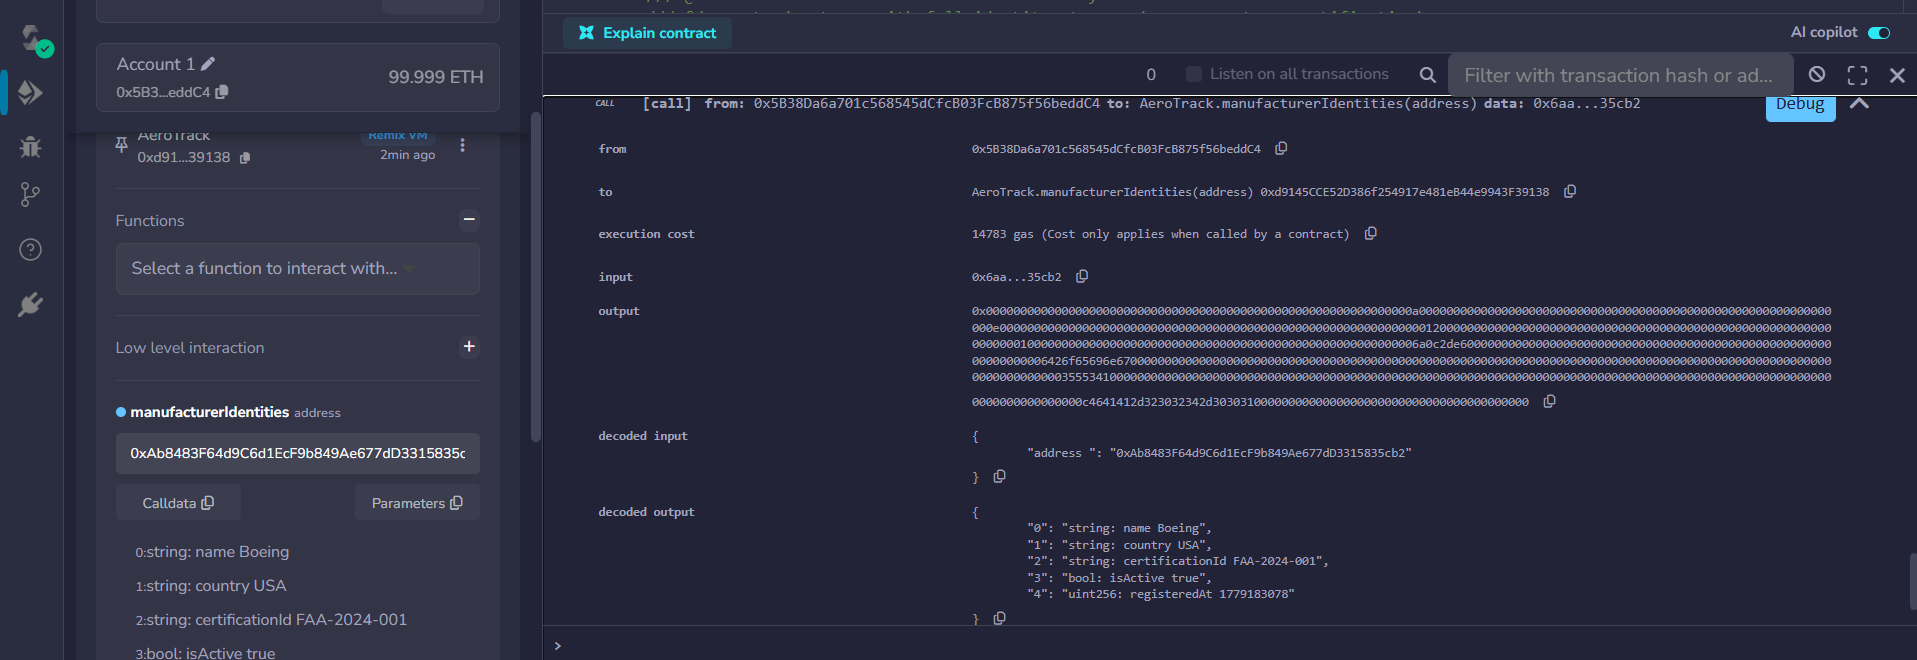
\includegraphics[width=0.85\textwidth]{../screens/step6-identity-query-account2.png}
    \caption{Querying \texttt{manufacturerIdentities} returns full on-chain identity}
    \label{fig:step6-identity}
\end{figure}

\begin{figure}[H]
    \centering
    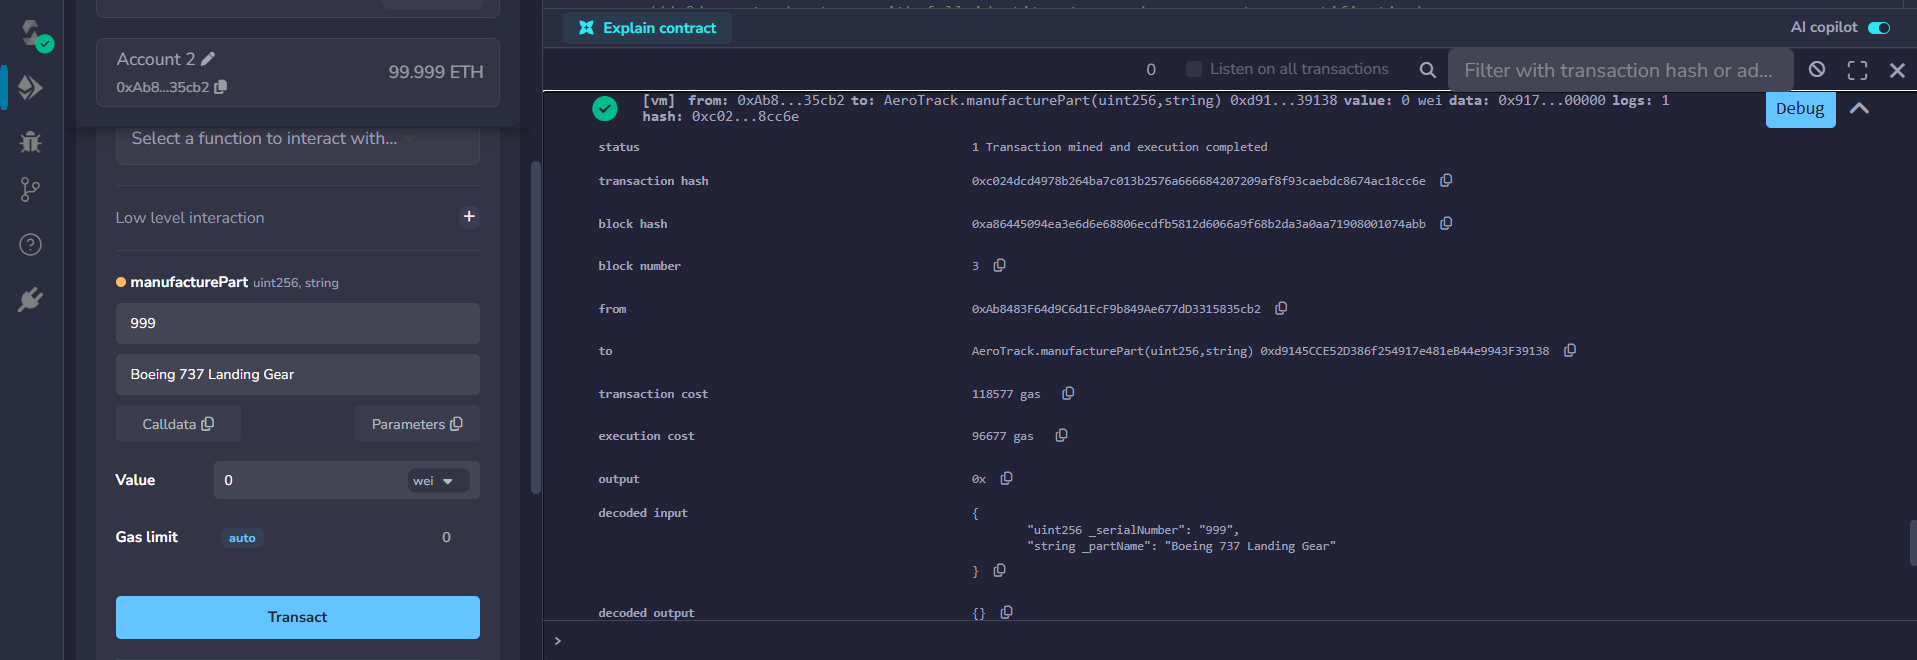
\includegraphics[width=0.85\textwidth]{../screens/step6-manufacturePart-success.png}
    \caption{Registered manufacturer successfully creates a part}
    \label{fig:step6-manufacture}
\end{figure}

\begin{figure}[H]
    \centering
    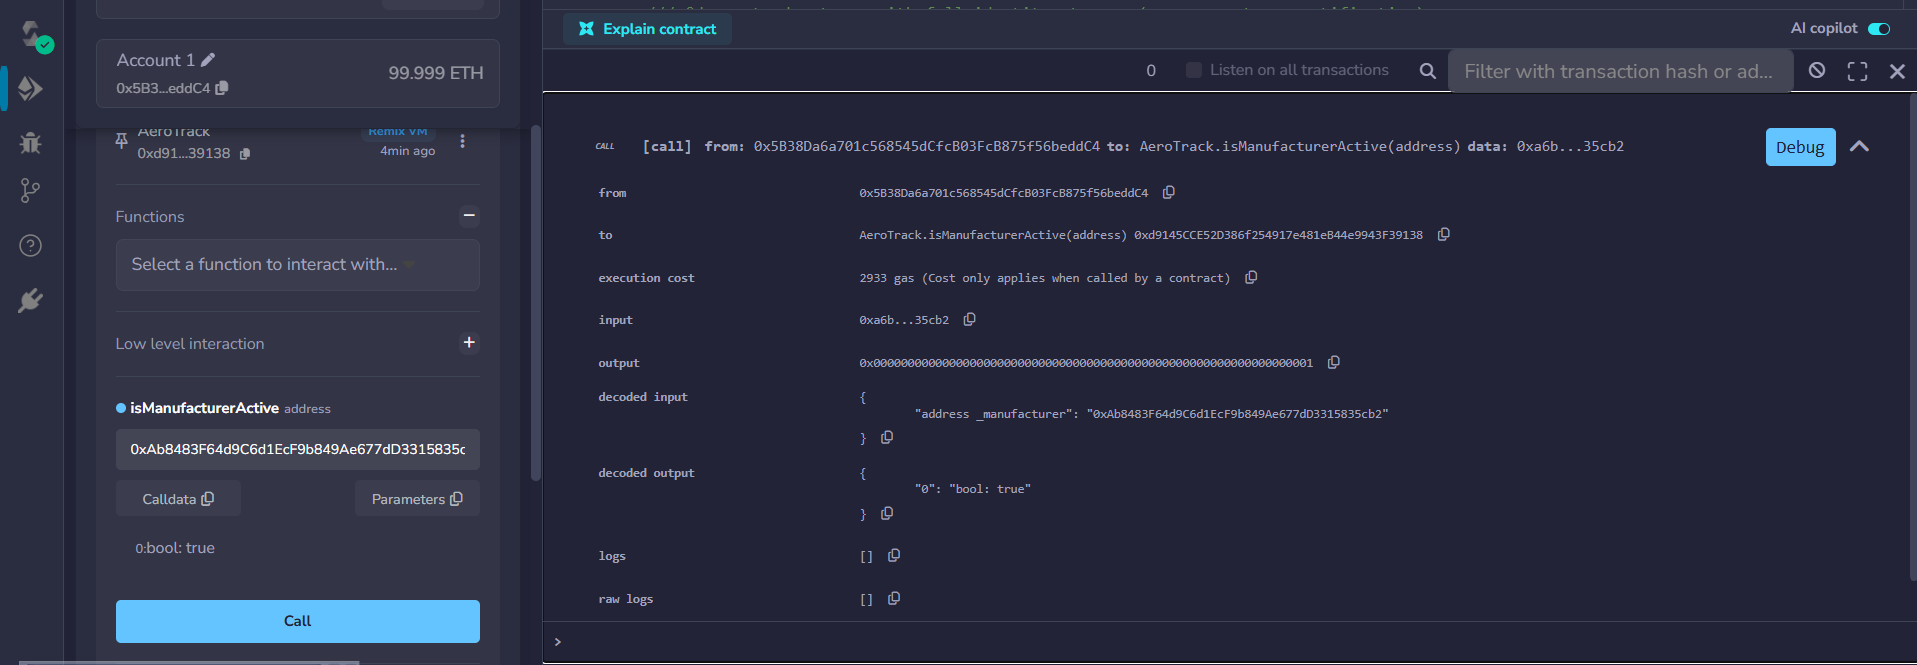
\includegraphics[width=0.85\textwidth]{../screens/step6-isManufacturerActive-true.png}
    \caption{\texttt{isManufacturerActive} returns true for registered manufacturer}
    \label{fig:step6-active}
\end{figure}

\begin{figure}[H]
    \centering
    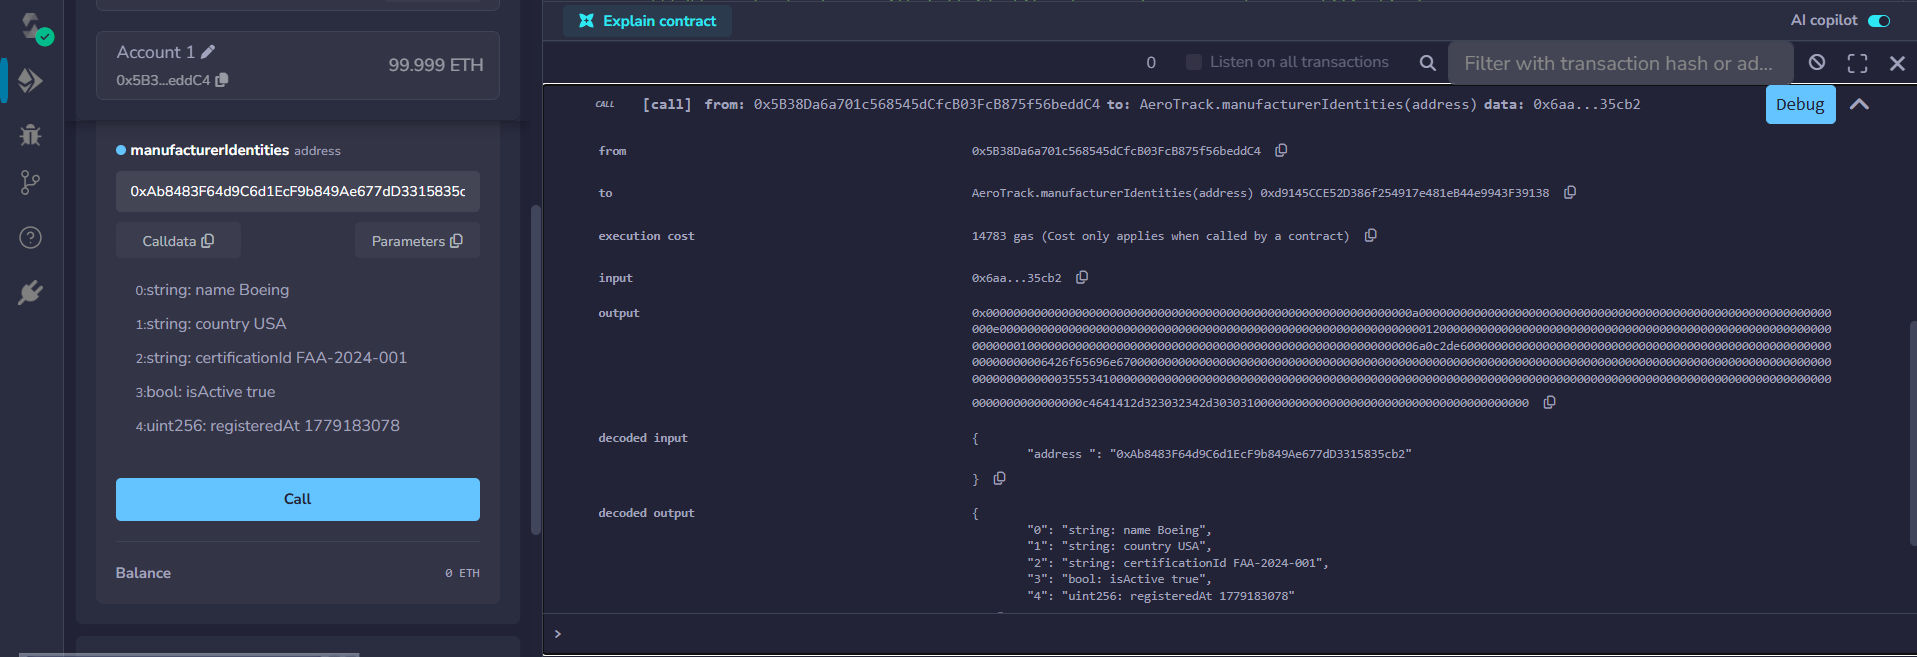
\includegraphics[width=0.85\textwidth]{../screens/step6-identity-verify.png}
    \caption{Public verification of manufacturer identity on-chain}
    \label{fig:step6-verify}
\end{figure}

\begin{figure}[H]
    \centering
    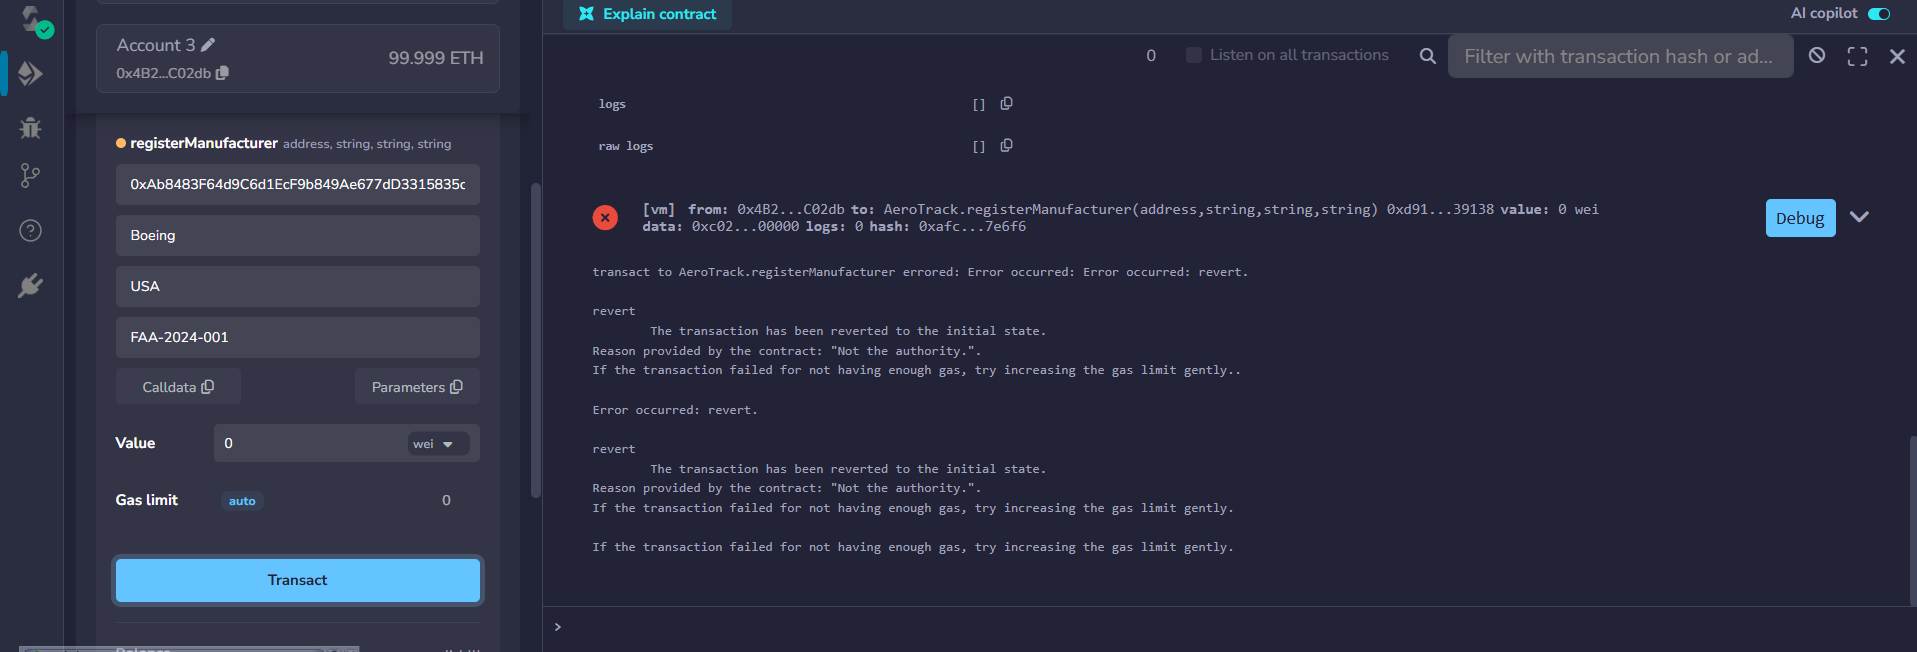
\includegraphics[width=0.85\textwidth]{../screens/step6-fail-register-account3.png}
    \caption{Unauthorized registration attempt fails (only authority can register)}
    \label{fig:step6-fail-register}
\end{figure}

\begin{figure}[H]
    \centering
    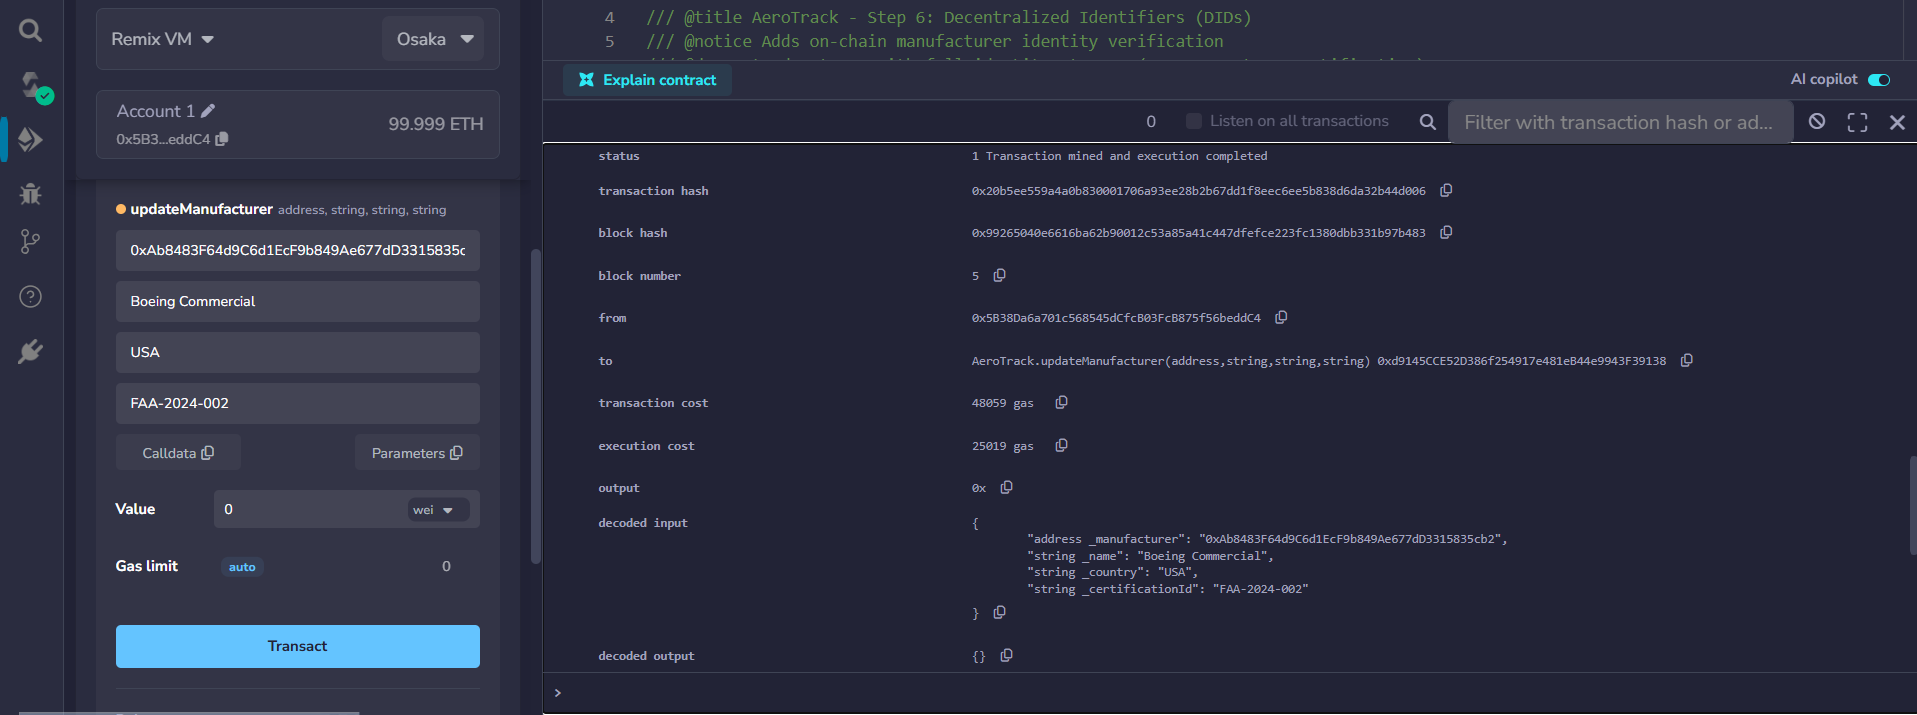
\includegraphics[width=0.85\textwidth]{../screens/step6-updateManufacturer.png}
    \caption{Authority updates manufacturer identity information}
    \label{fig:step6-update}
\end{figure}

\begin{figure}[H]
    \centering
    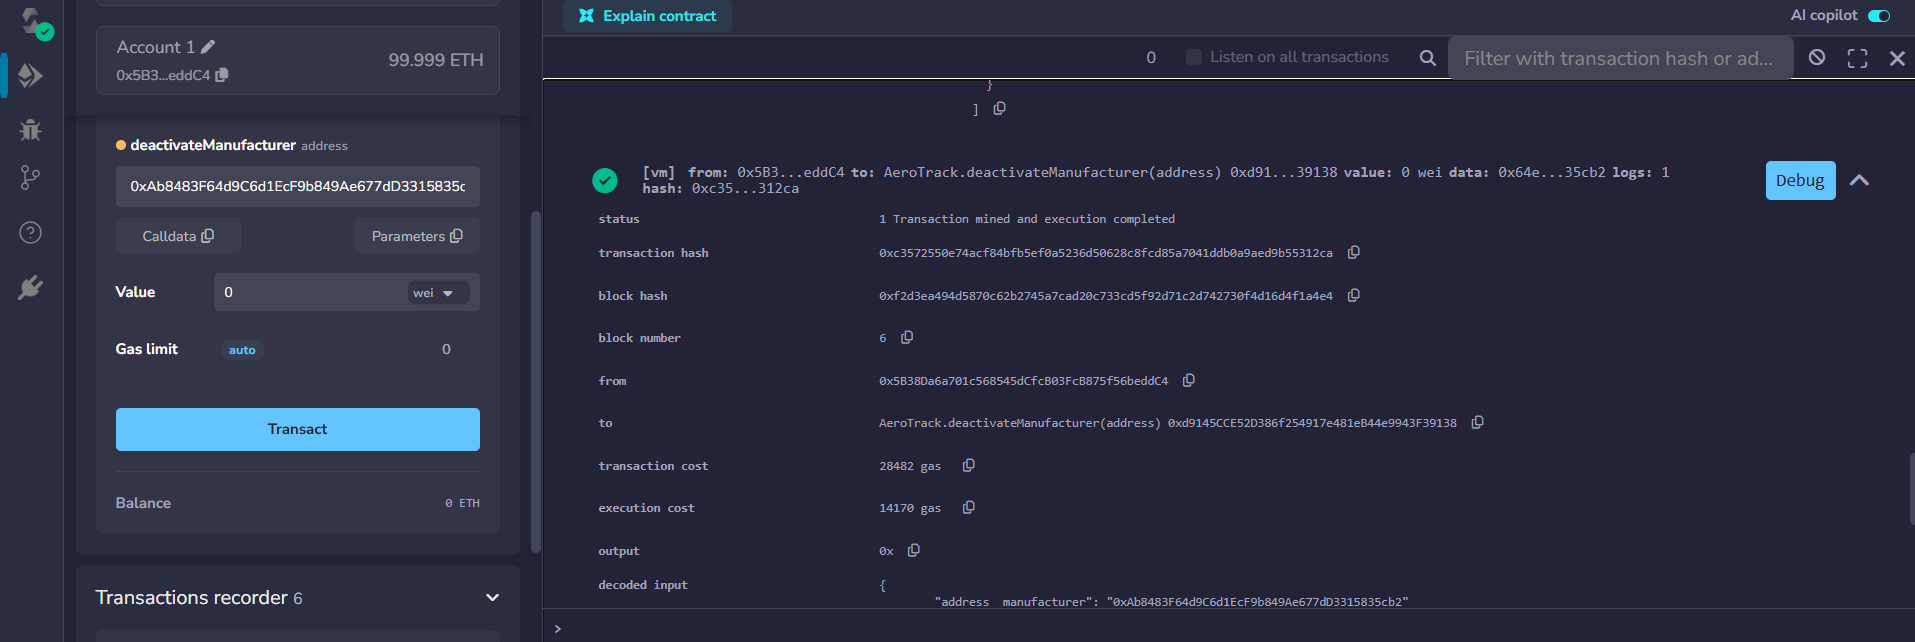
\includegraphics[width=0.85\textwidth]{../screens/step6-deactivateManufacturer.png}
    \caption{Authority deactivates manufacturer (DID revocation)}
    \label{fig:step6-deactivate}
\end{figure}

\begin{figure}[H]
    \centering
    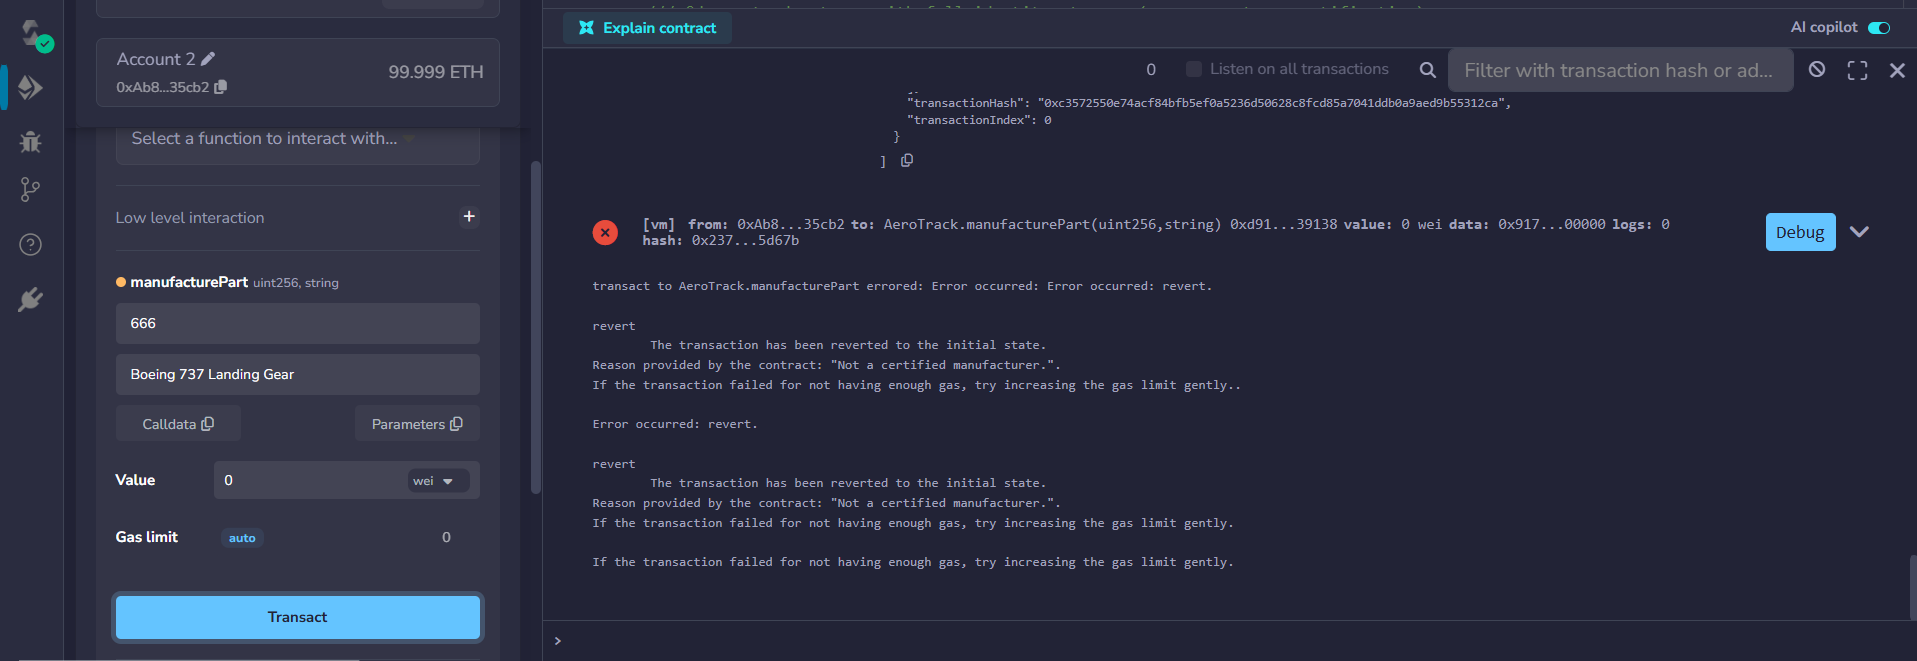
\includegraphics[width=0.85\textwidth]{../screens/step6-fail-after-deactivate.png}
    \caption{Deactivated manufacturer fails to create parts}
    \label{fig:step6-fail-deactivate}
\end{figure}

% ============================================================
\subsection{Step 7: IoT Oracle Simulation}
% ============================================================

To address the \textbf{IoT Oracles} research topic, we implemented an authorized sensor system. Physical IoT devices (simulated by Remix accounts) can automatically report maintenance data for their assigned parts without human intervention.

\begin{lstlisting}[caption={IoT Sensor struct and registration}]
struct Sensor {
    uint256 assignedPart;    // Which part this sensor monitors
    string sensorType;       // "temperature", "vibration", "stress"
    bool isActive;
    uint256 registeredAt;
}

mapping(address => Sensor) public sensors;

modifier onlyActiveSensor() {
    require(sensors[msg.sender].isActive, "Not an authorized sensor.");
    _;
}

function registerSensor(address _sensor, uint256 _sn,
    string memory _type) public onlyAuthority partExists(_sn) {
    sensors[_sensor] = Sensor(_sn, _type, true, block.timestamp);
    emit SensorRegistered(_sensor, _sn, _type);
}

function logSensorData(string memory _dataType,
    string memory _value) public onlyActiveSensor {
    uint256 sn = sensors[msg.sender].assignedPart;
    emit SensorDataLogged(sn, msg.sender, _dataType, _value);
}
\end{lstlisting}

The sensor does not pass the serial number --- it is automatically resolved from the registry. This prevents a sensor from reporting data for parts it is not assigned to.

\begin{figure}[H]
    \centering
    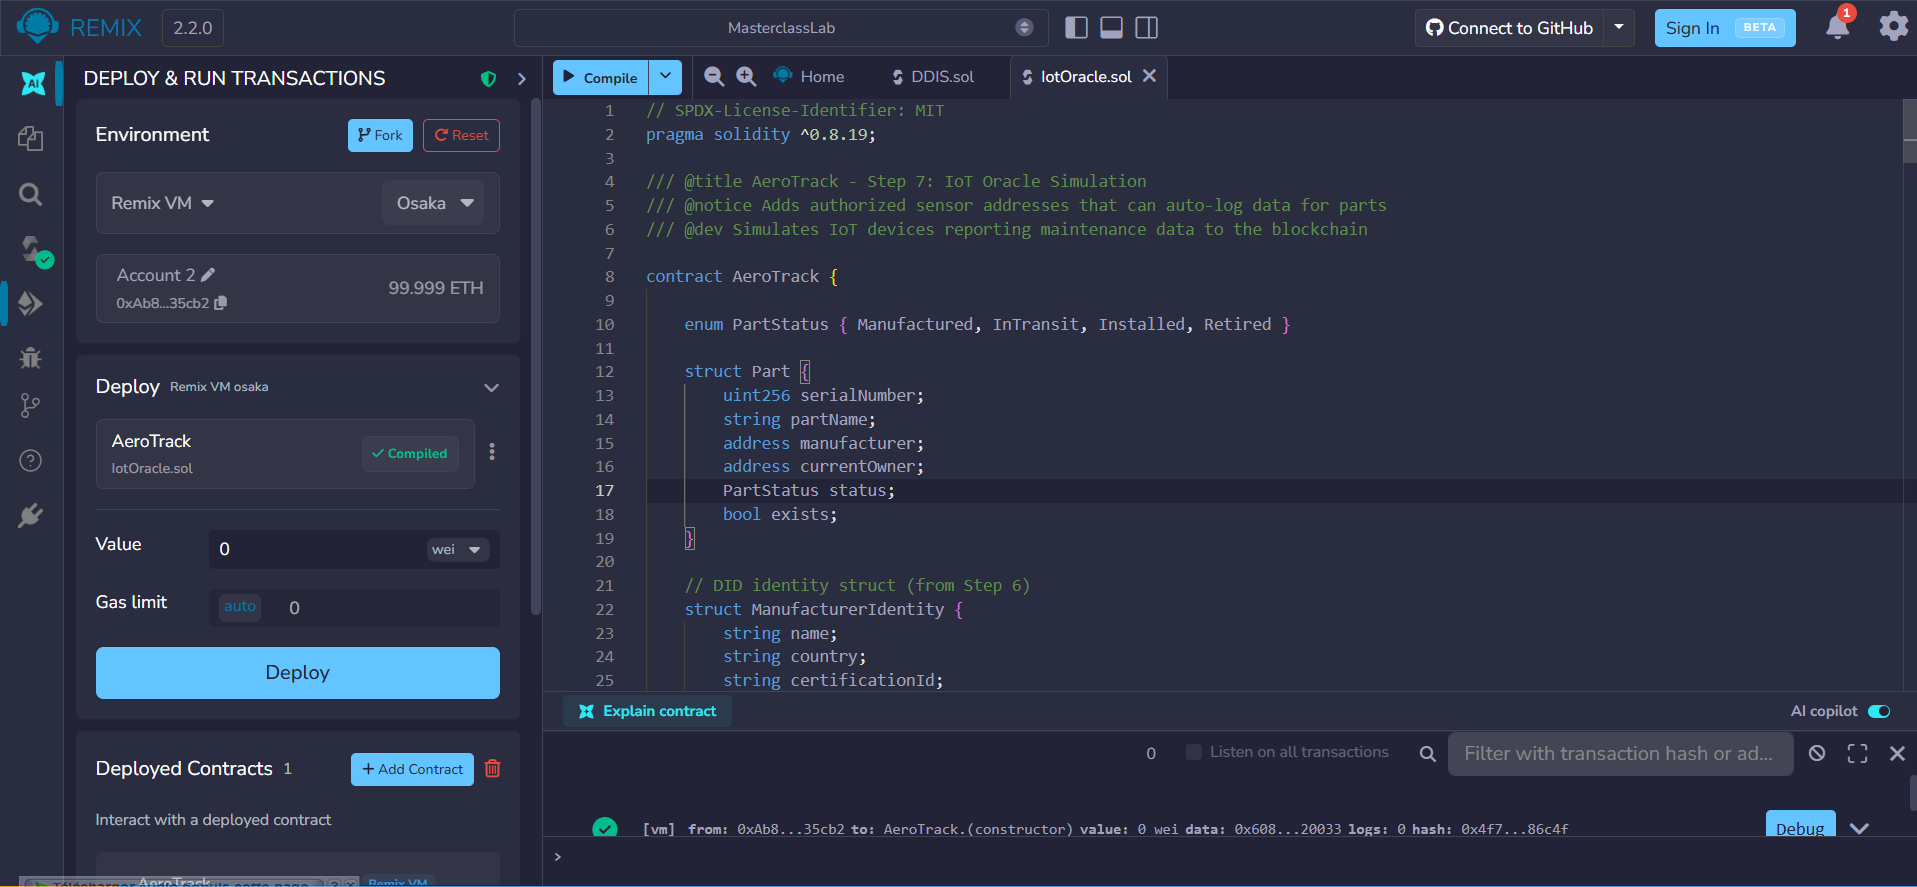
\includegraphics[width=0.85\textwidth]{../screens/step7-code.png}
    \caption{IoT Oracle contract code in Remix}
    \label{fig:step7-code}
\end{figure}

\begin{figure}[H]
    \centering
    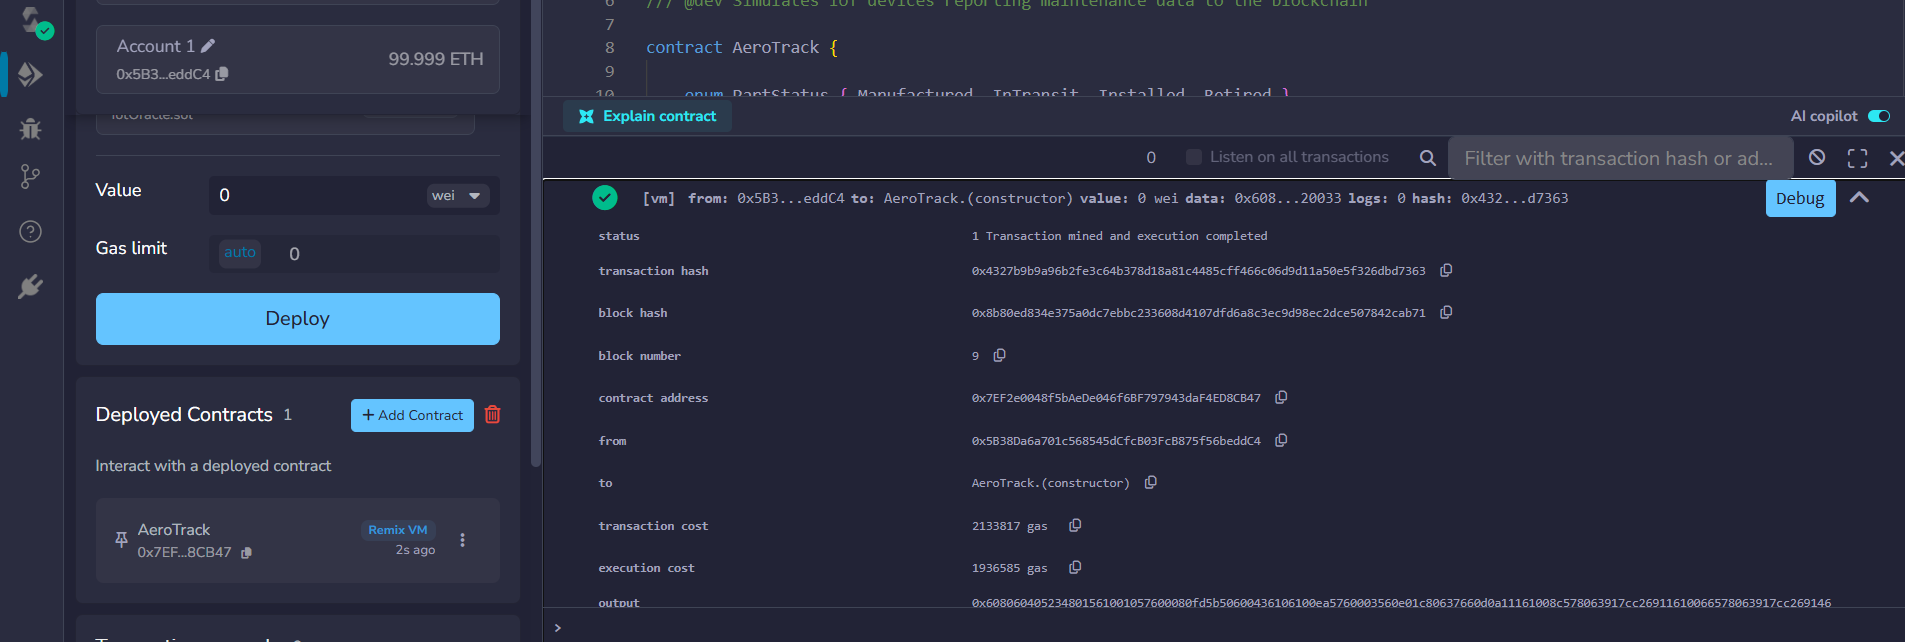
\includegraphics[width=0.85\textwidth]{../screens/step7-deploy-success.png}
    \caption{Successful deployment of the IoT-enhanced contract}
    \label{fig:step7-deploy}
\end{figure}

\begin{figure}[H]
    \centering
    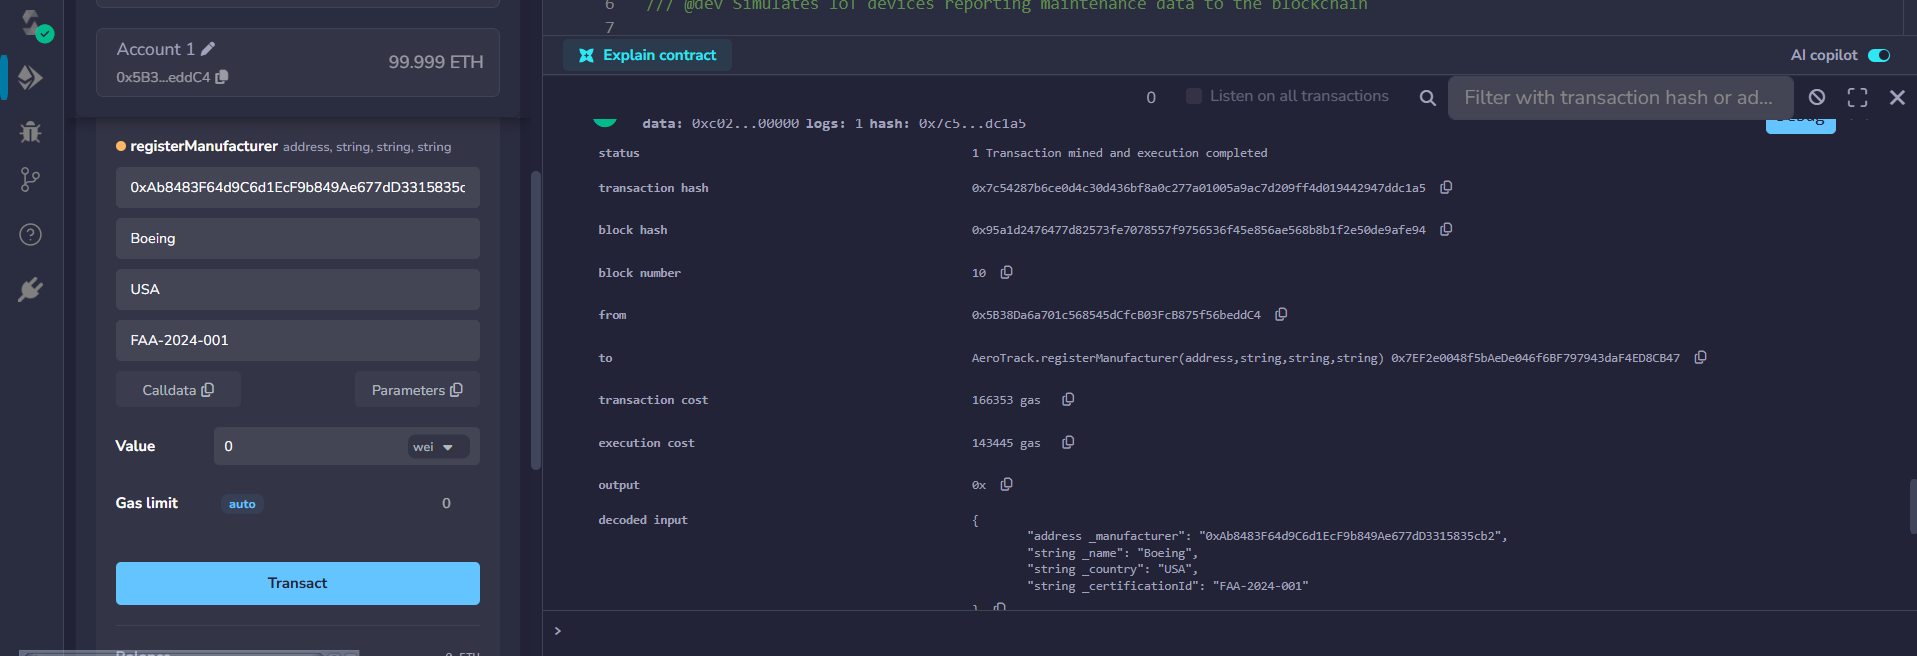
\includegraphics[width=0.85\textwidth]{../screens/step7-registerManufacturer.png}
    \caption{Registering Boeing as a certified manufacturer}
    \label{fig:step7-regmfr}
\end{figure}

\begin{figure}[H]
    \centering
    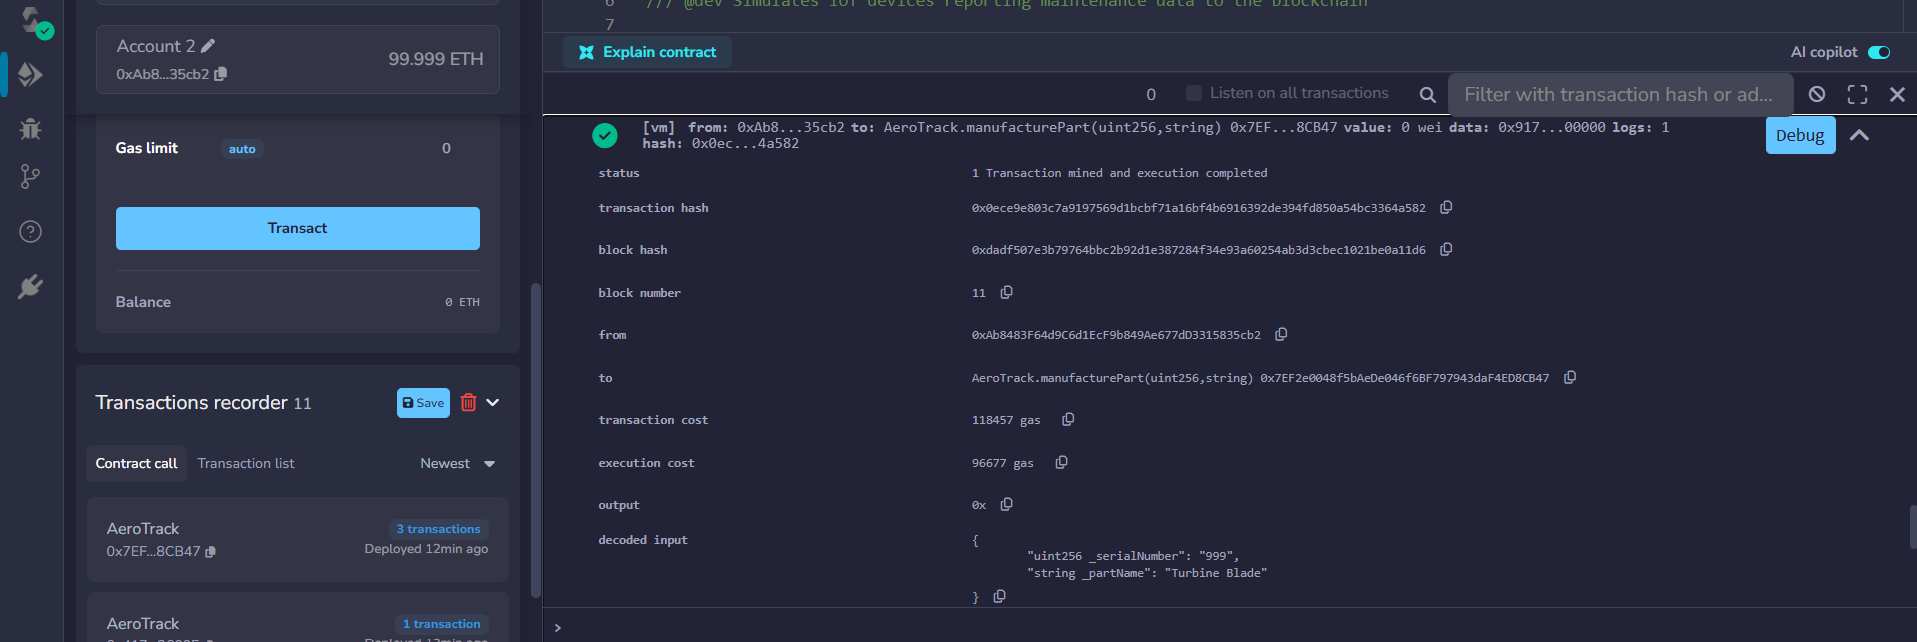
\includegraphics[width=0.85\textwidth]{../screens/step7-manufacturePart.png}
    \caption{Account 2 (Boeing) manufactures part 999}
    \label{fig:step7-mfr}
\end{figure}

\begin{figure}[H]
    \centering
    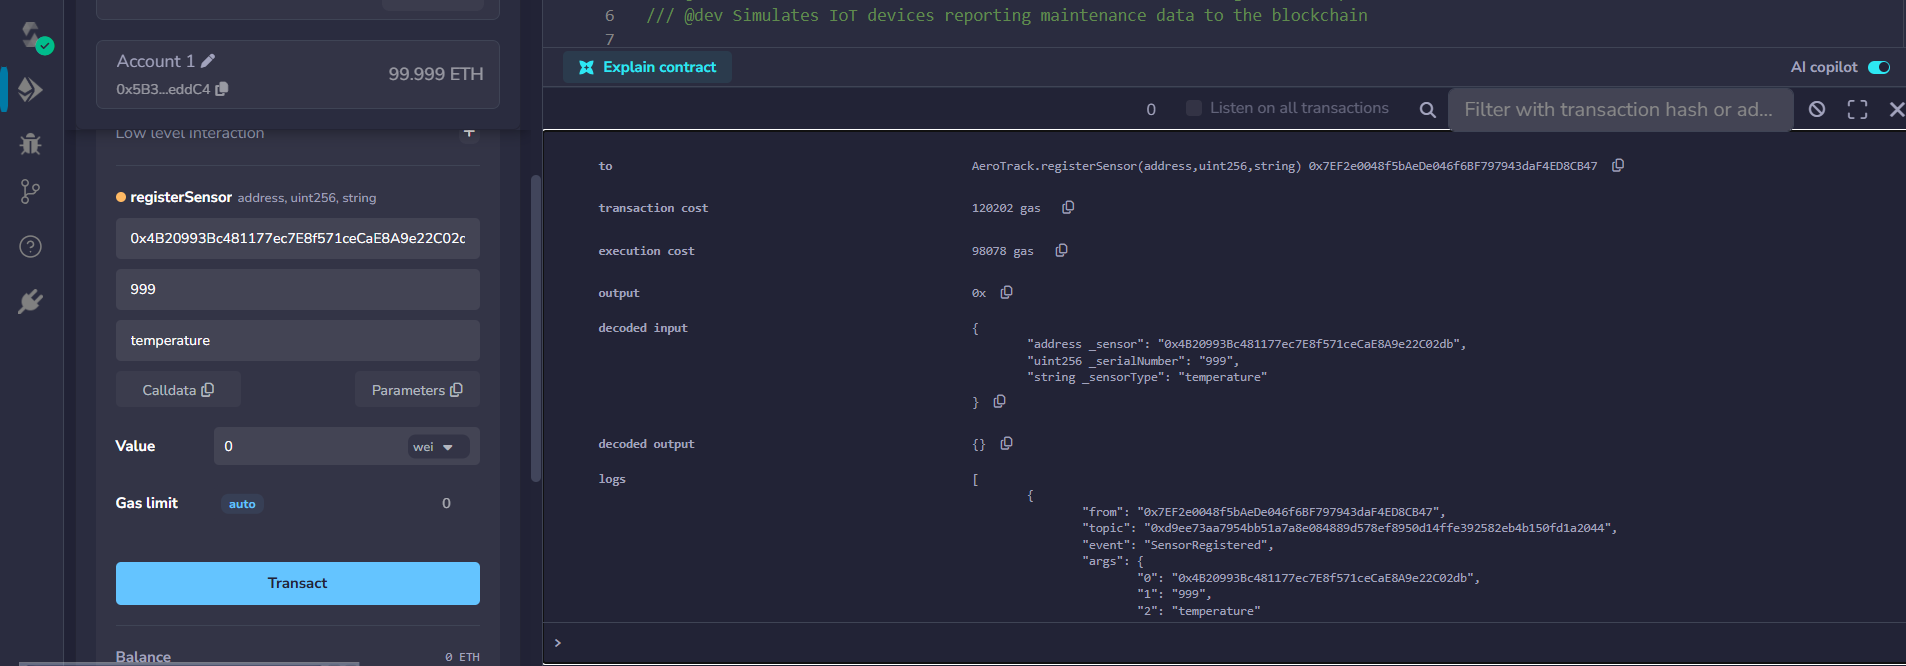
\includegraphics[width=0.85\textwidth]{../screens/step7-registerSensor.png}
    \caption{Authority registers Account 3 as a temperature sensor for part 999}
    \label{fig:step7-regsensor}
\end{figure}

\begin{figure}[H]
    \centering
    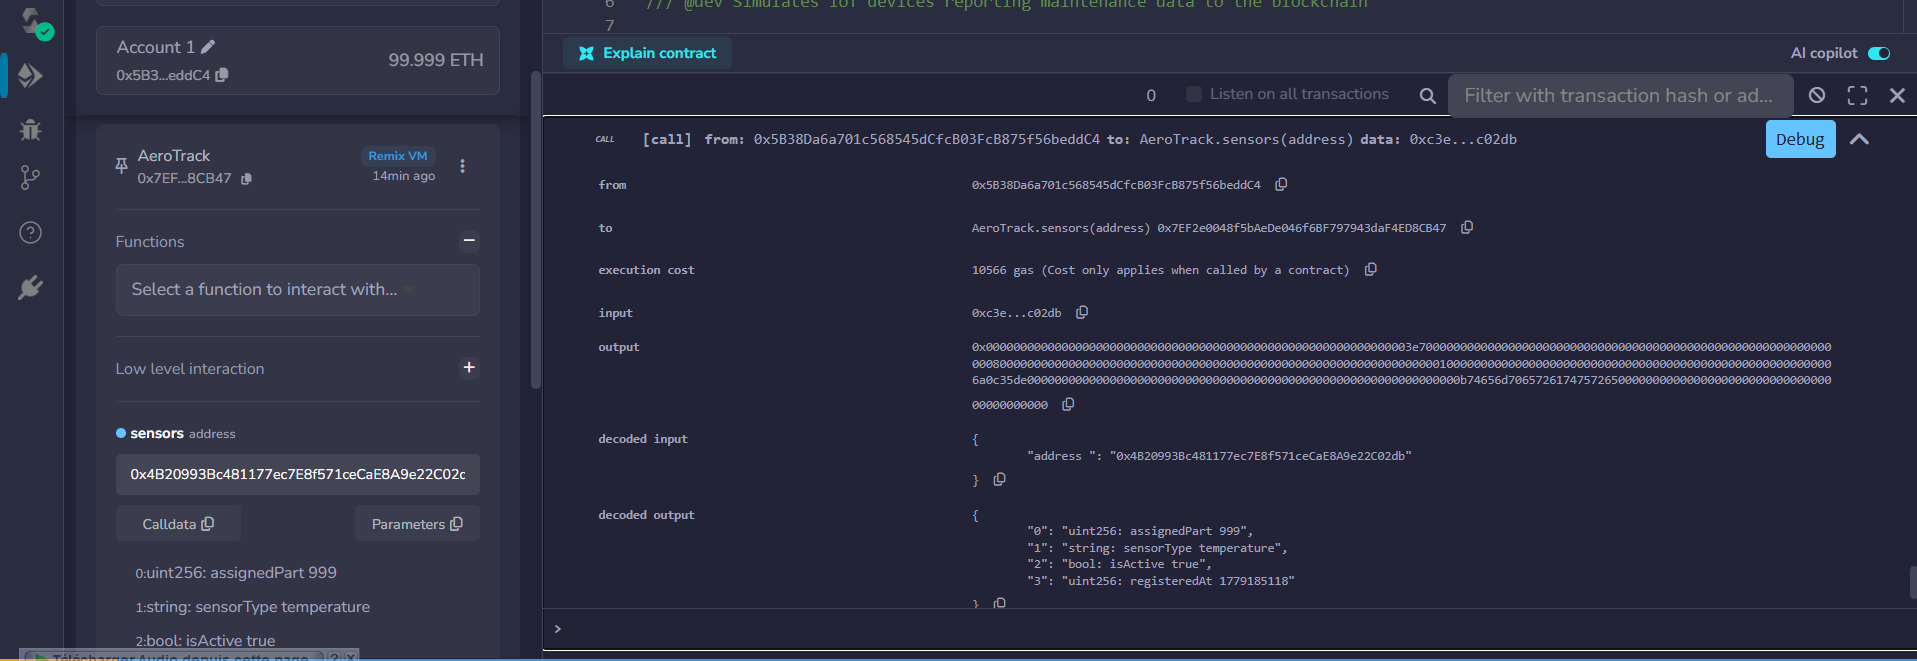
\includegraphics[width=0.85\textwidth]{../screens/step7-sensors-query.png}
    \caption{Querying \texttt{sensors} shows assigned part and sensor type}
    \label{fig:step7-query}
\end{figure}

\begin{figure}[H]
    \centering
    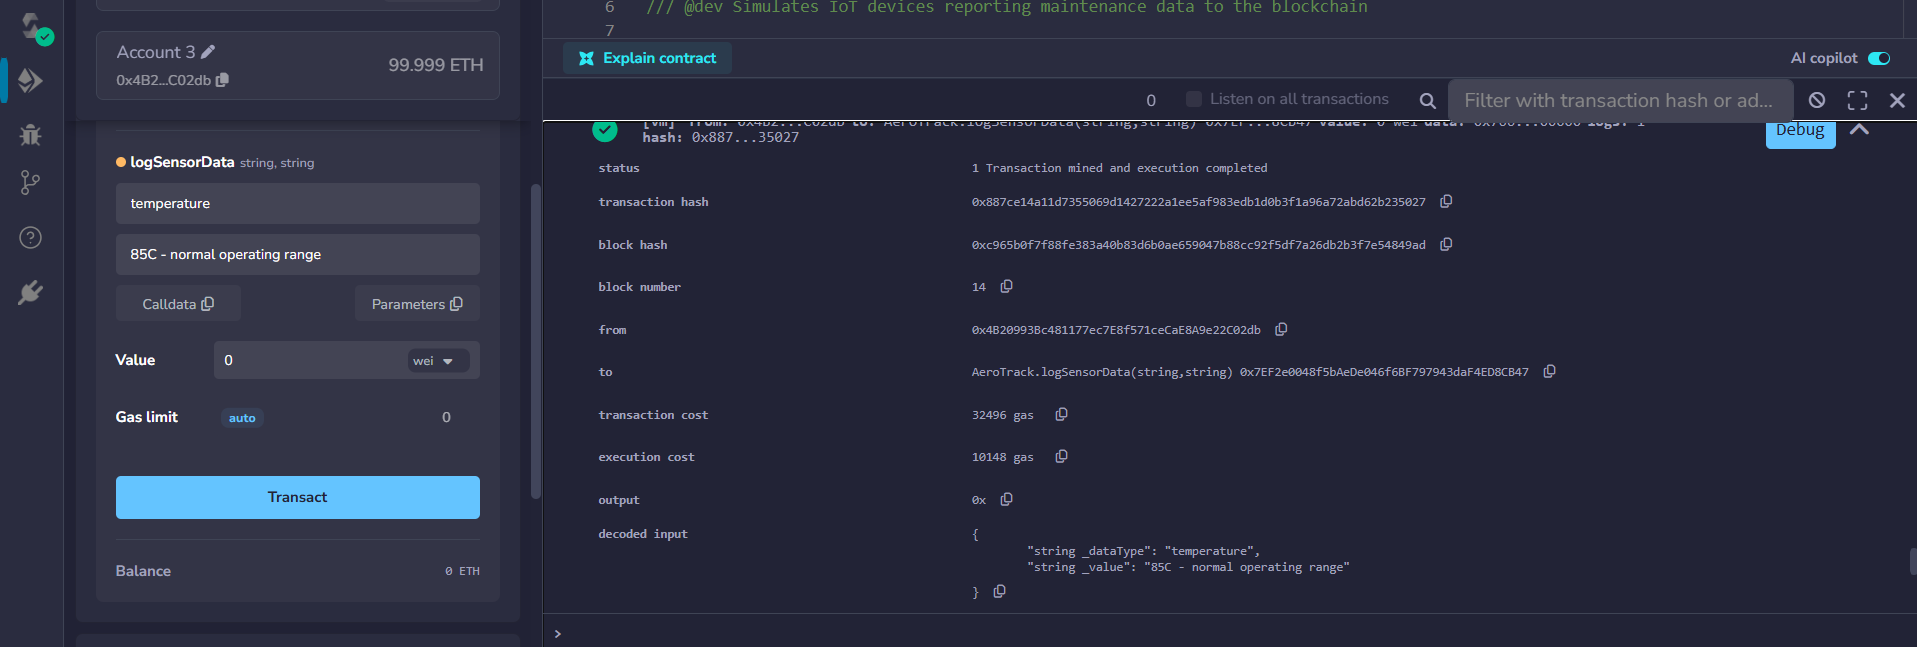
\includegraphics[width=0.85\textwidth]{../screens/step7-sensorData-temperature.png}
    \caption{Sensor reports temperature reading via \texttt{logSensorData}}
    \label{fig:step7-temp}
\end{figure}

\begin{figure}[H]
    \centering
    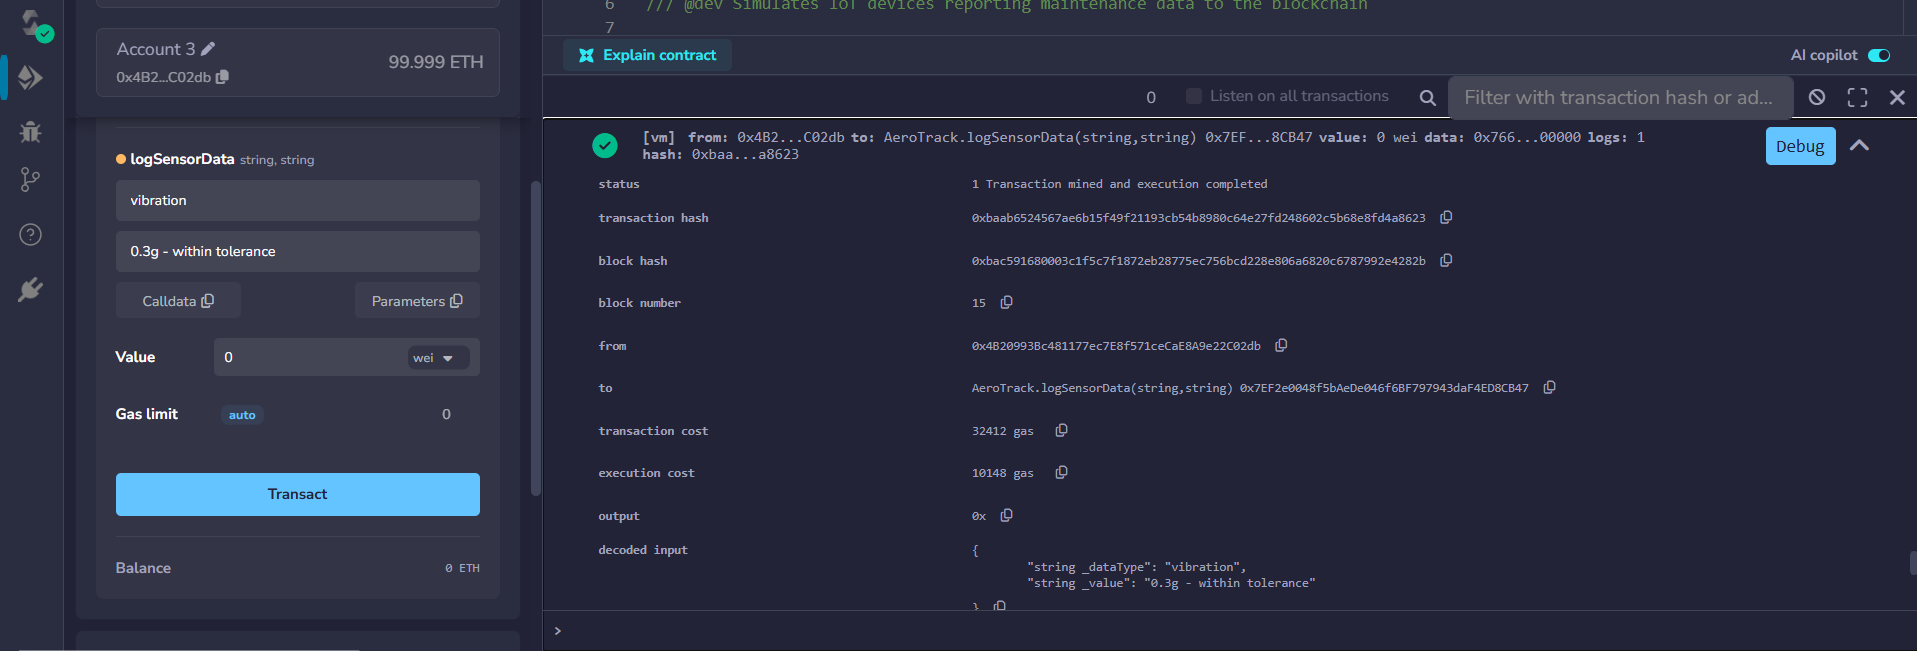
\includegraphics[width=0.85\textwidth]{../screens/step7-sensorData-vibration.png}
    \caption{Sensor reports vibration reading}
    \label{fig:step7-vibration}
\end{figure}

\begin{figure}[H]
    \centering
    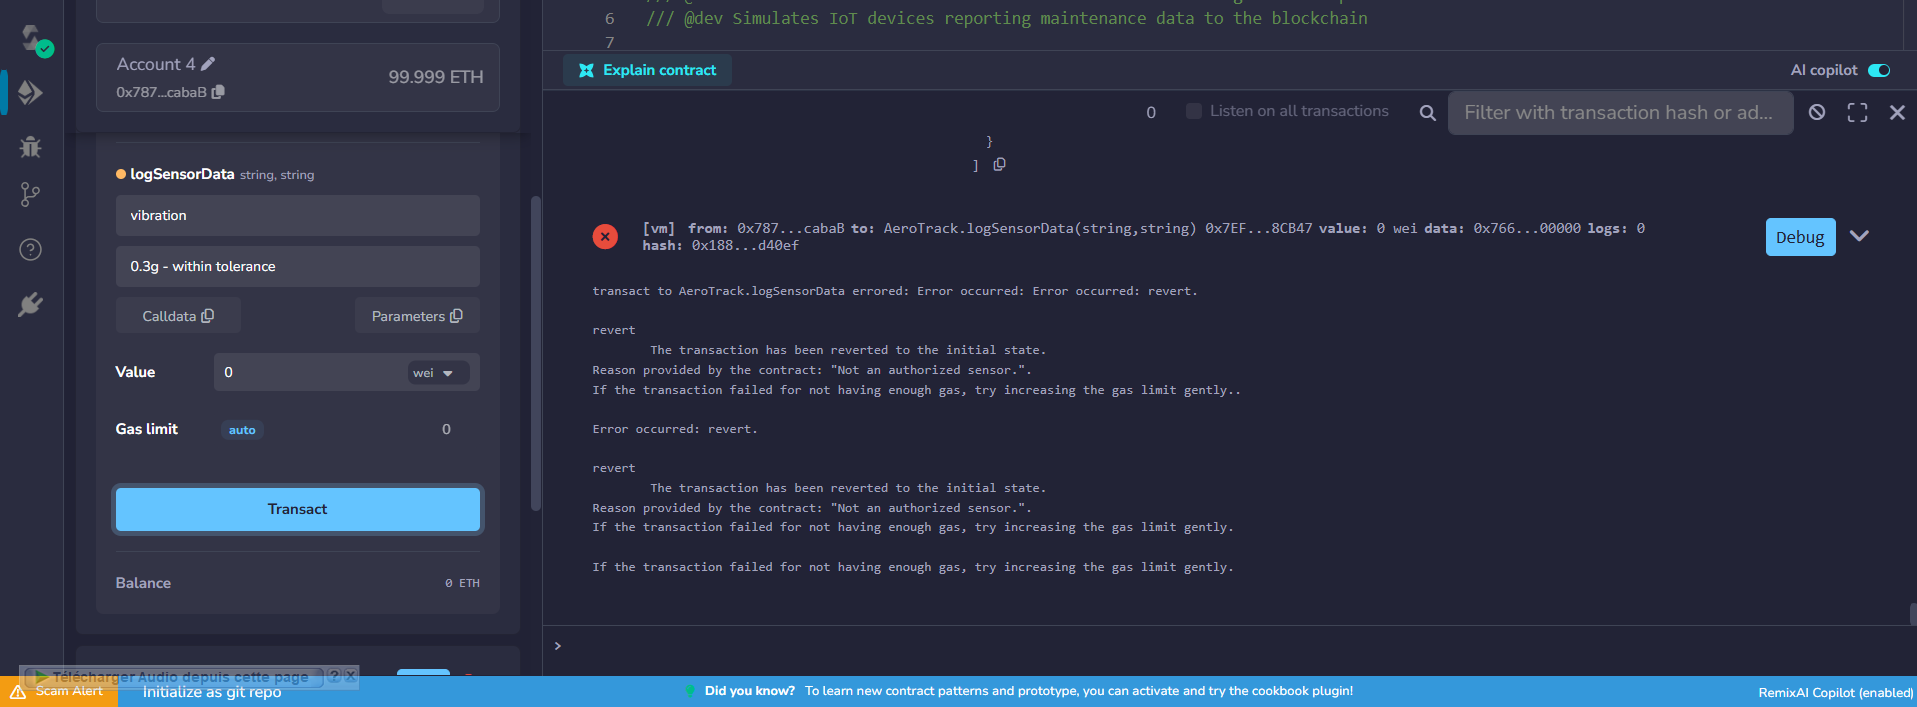
\includegraphics[width=0.85\textwidth]{../screens/step7-fail-unauthorized-account2.png}
    \caption{Unauthorized Account 2 fails to log sensor data}
    \label{fig:step7-fail-unauth}
\end{figure}

\begin{figure}[H]
    \centering
    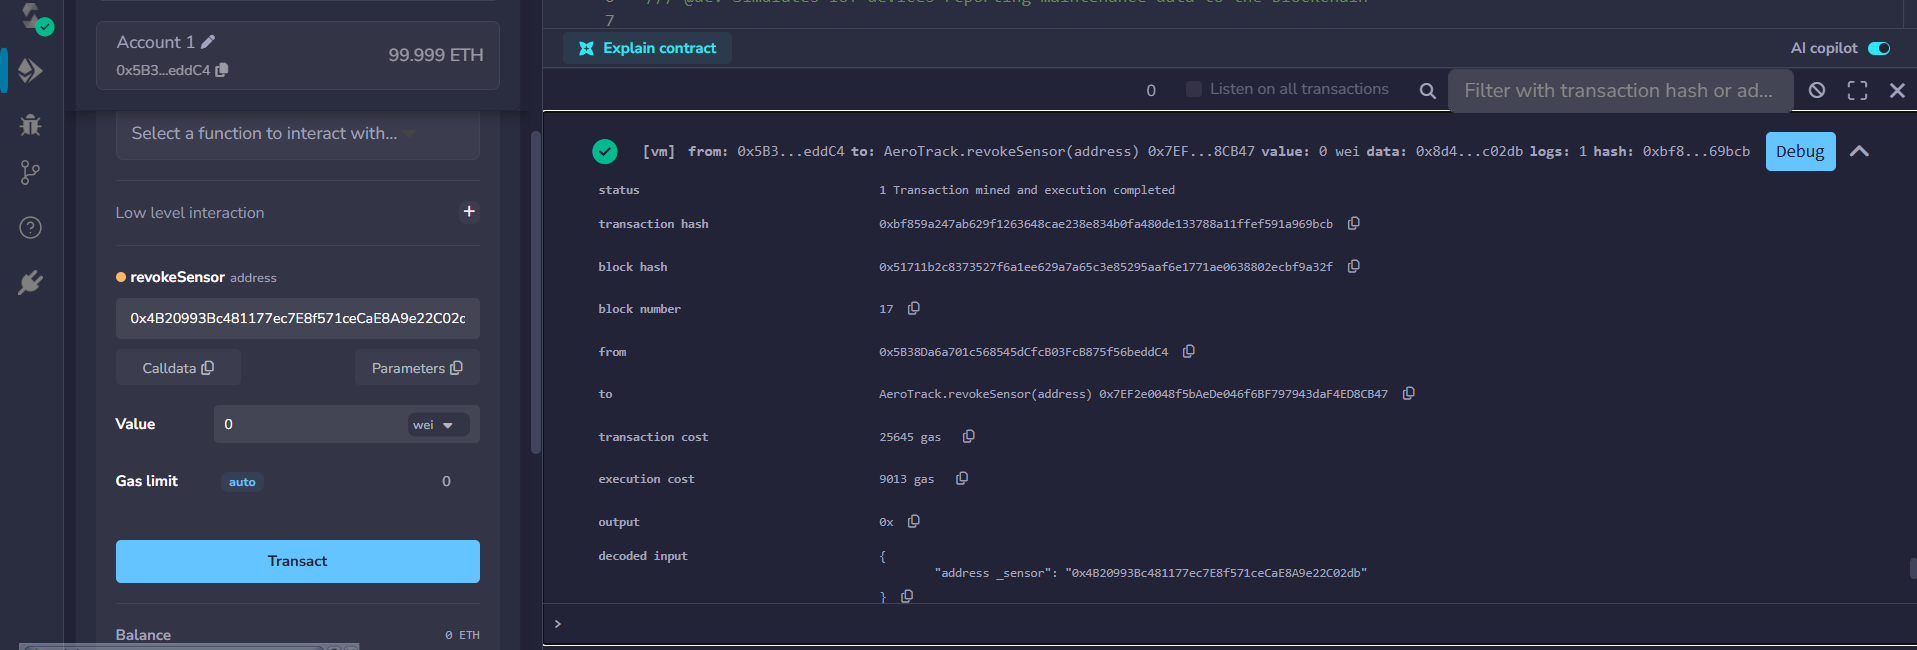
\includegraphics[width=0.85\textwidth]{../screens/step7-revokeSensor.png}
    \caption{Authority revokes sensor authorization from Account 3}
    \label{fig:step7-revoke}
\end{figure}

\begin{figure}[H]
    \centering
    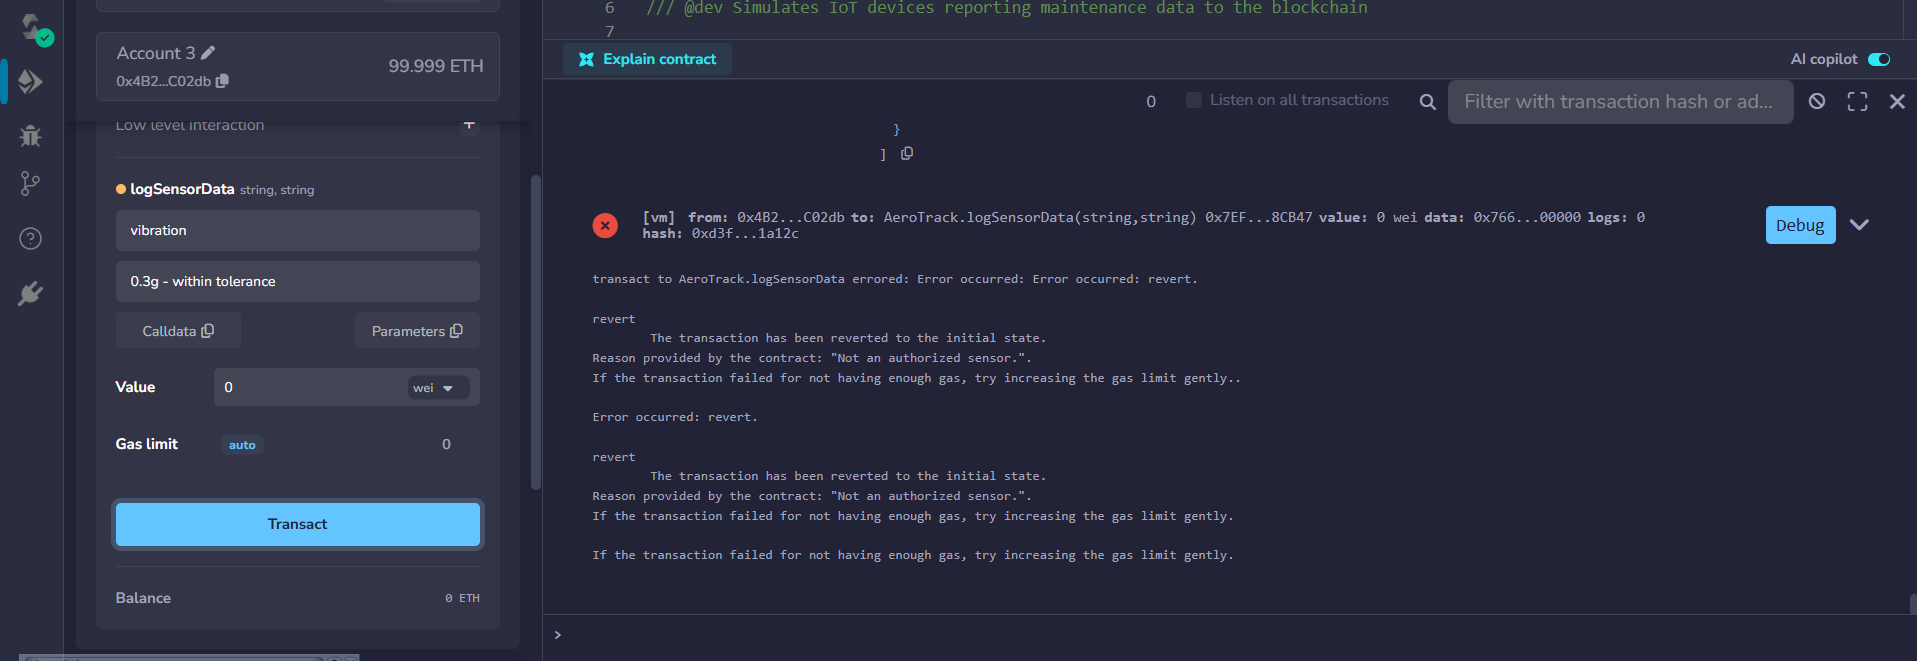
\includegraphics[width=0.85\textwidth]{../screens/step7-fail-after-revoke.png}
    \caption{Revoked sensor (Account 3) fails to report data}
    \label{fig:step7-fail-revoke}
\end{figure}

% ============================================================
\subsection{Step 8: Real IoT Oracle with MQTT Broker}
% ============================================================

To demonstrate a production-ready architecture, we implemented a full IoT pipeline using \textbf{MQTT} (Message Queuing Telemetry Transport) as the communication protocol between sensors and the blockchain. The system uses Docker containers for the MQTT broker (Mosquitto) and a local Ethereum node (Ganache).

The architecture follows the oracle pattern:
\begin{enumerate}
    \item A Python sensor simulator publishes temperature readings to the MQTT broker
    \item A Node.js bridge subscribes to the MQTT topic
    \item When data arrives, the bridge signs a transaction and calls \texttt{logSensorData()} on the smart contract
    \item The blockchain permanently records the sensor reading as an event
\end{enumerate}

\begin{figure}[H]
    \centering
    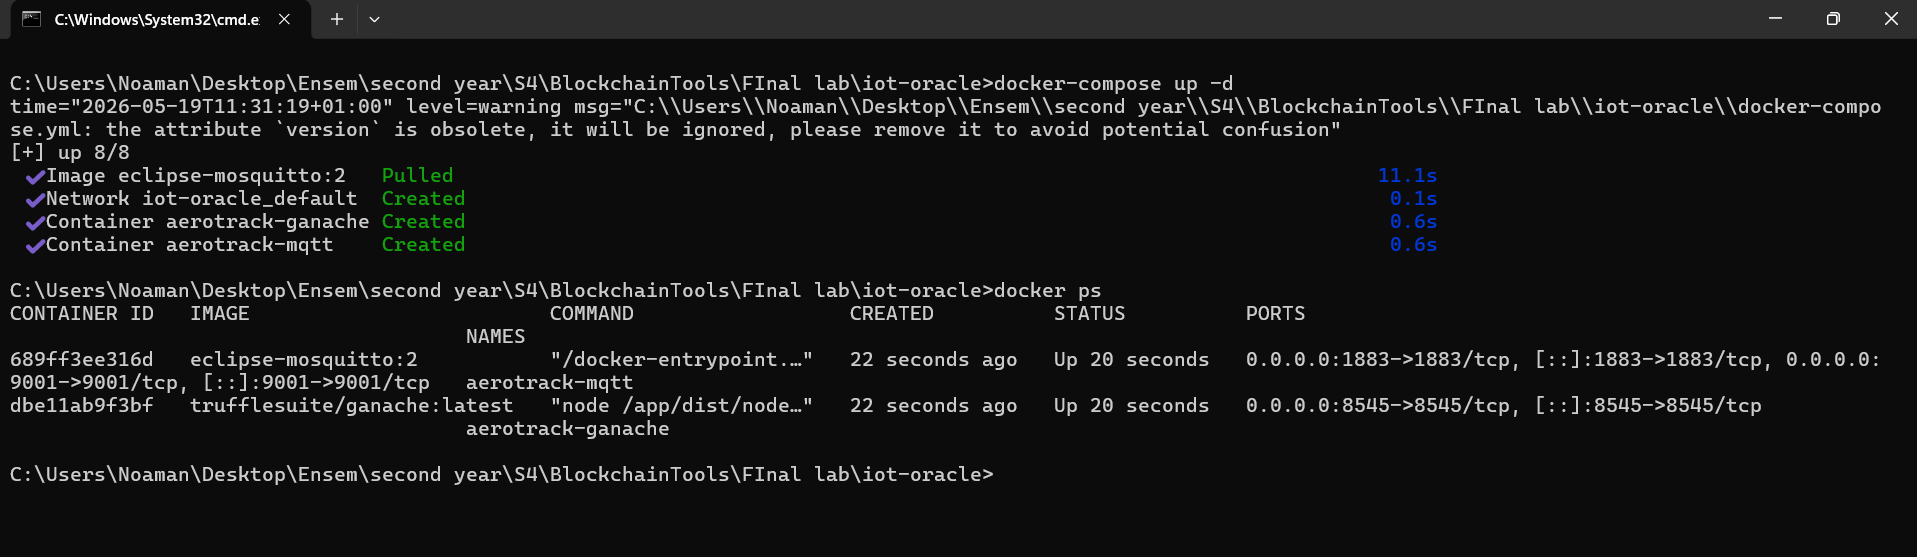
\includegraphics[width=0.85\textwidth]{../screens/step8-deploy-ganache.png}
    \caption{Contract deployed on Ganache via Remix (External Http Provider)}
    \label{fig:step8-deploy}
\end{figure}

\begin{figure}[H]
    \centering
    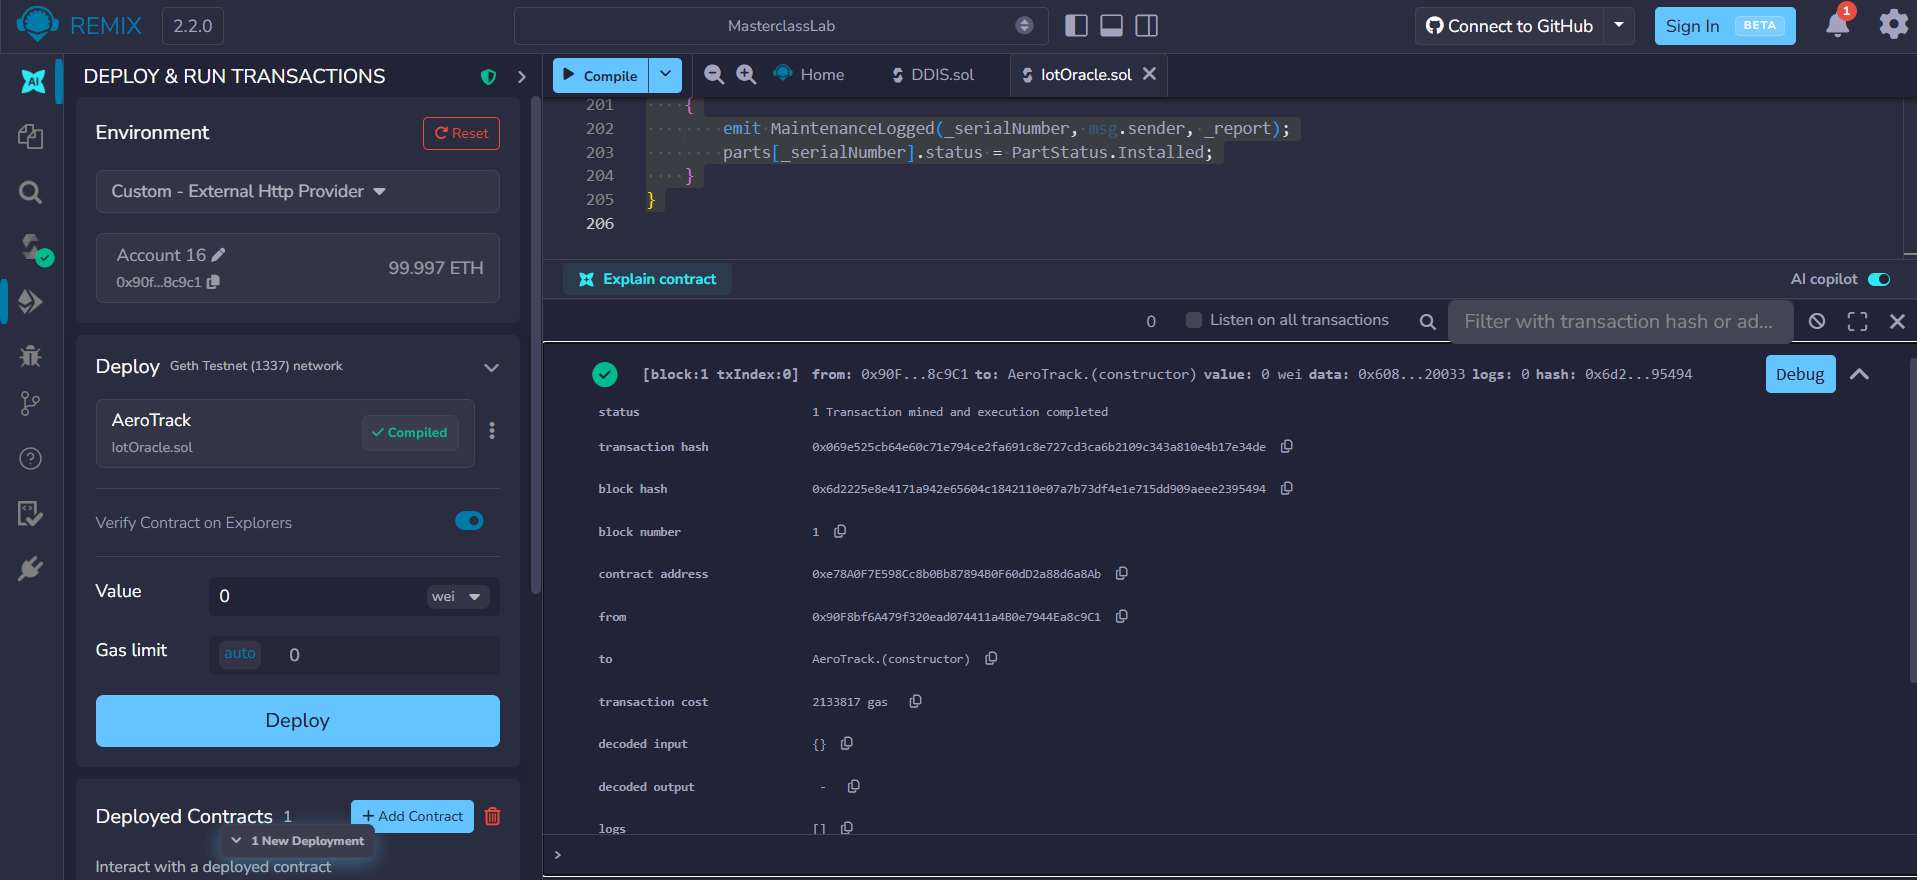
\includegraphics[width=0.85\textwidth]{../screens/step8-registerManufacturer.png}
    \caption{Registering manufacturer on Ganache blockchain}
    \label{fig:step8-regmfr}
\end{figure}

\begin{figure}[H]
    \centering
    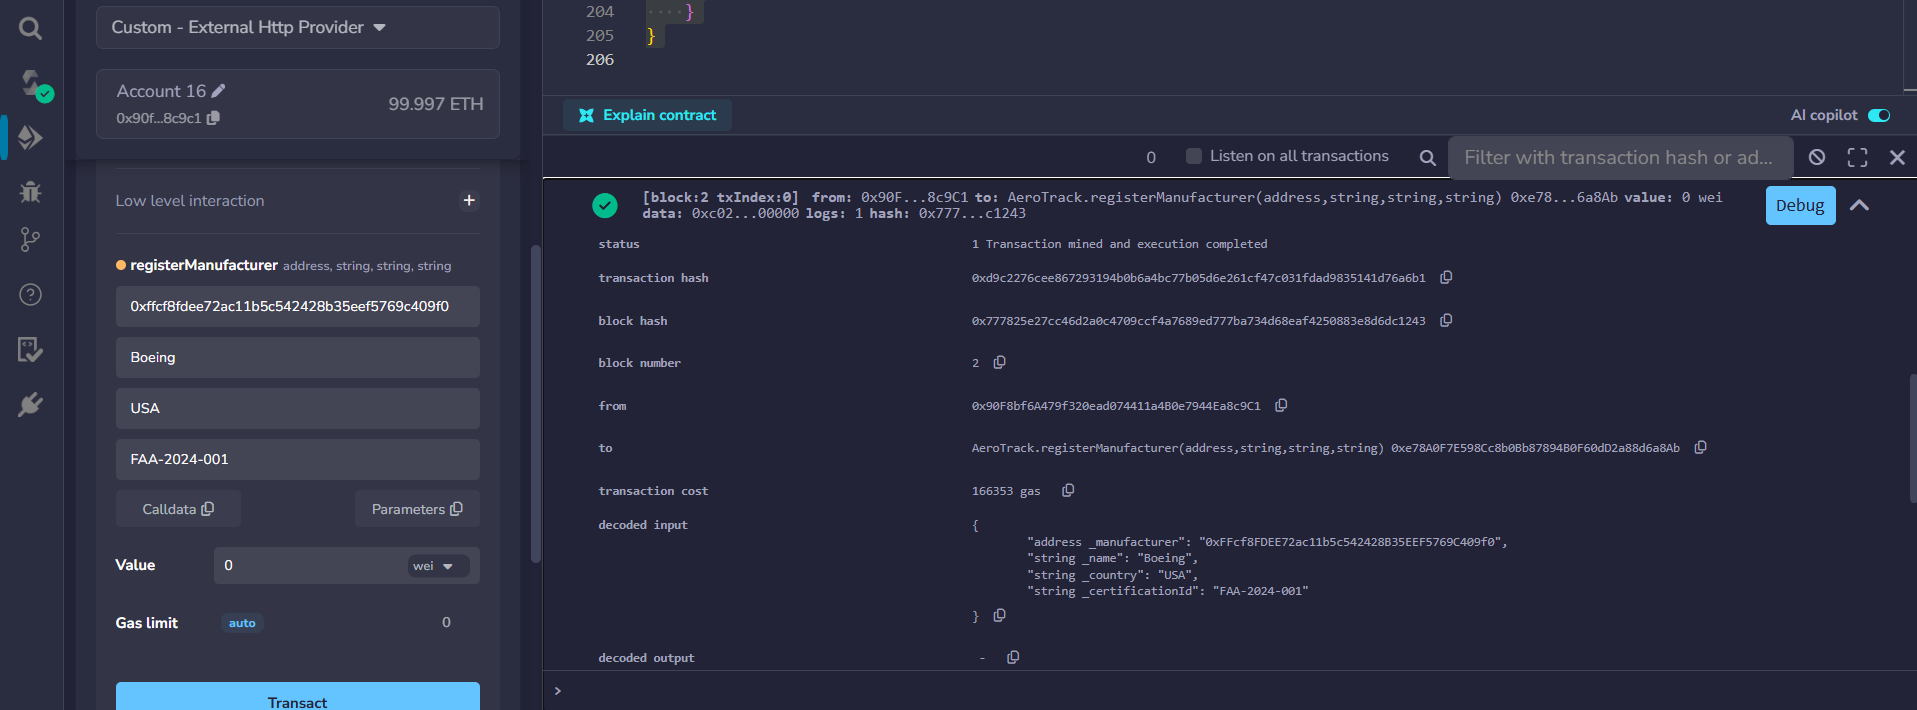
\includegraphics[width=0.85\textwidth]{../screens/step8-manufacturePart.png}
    \caption{Manufacturing part 999 on Ganache}
    \label{fig:step8-mfr}
\end{figure}

\begin{figure}[H]
    \centering
    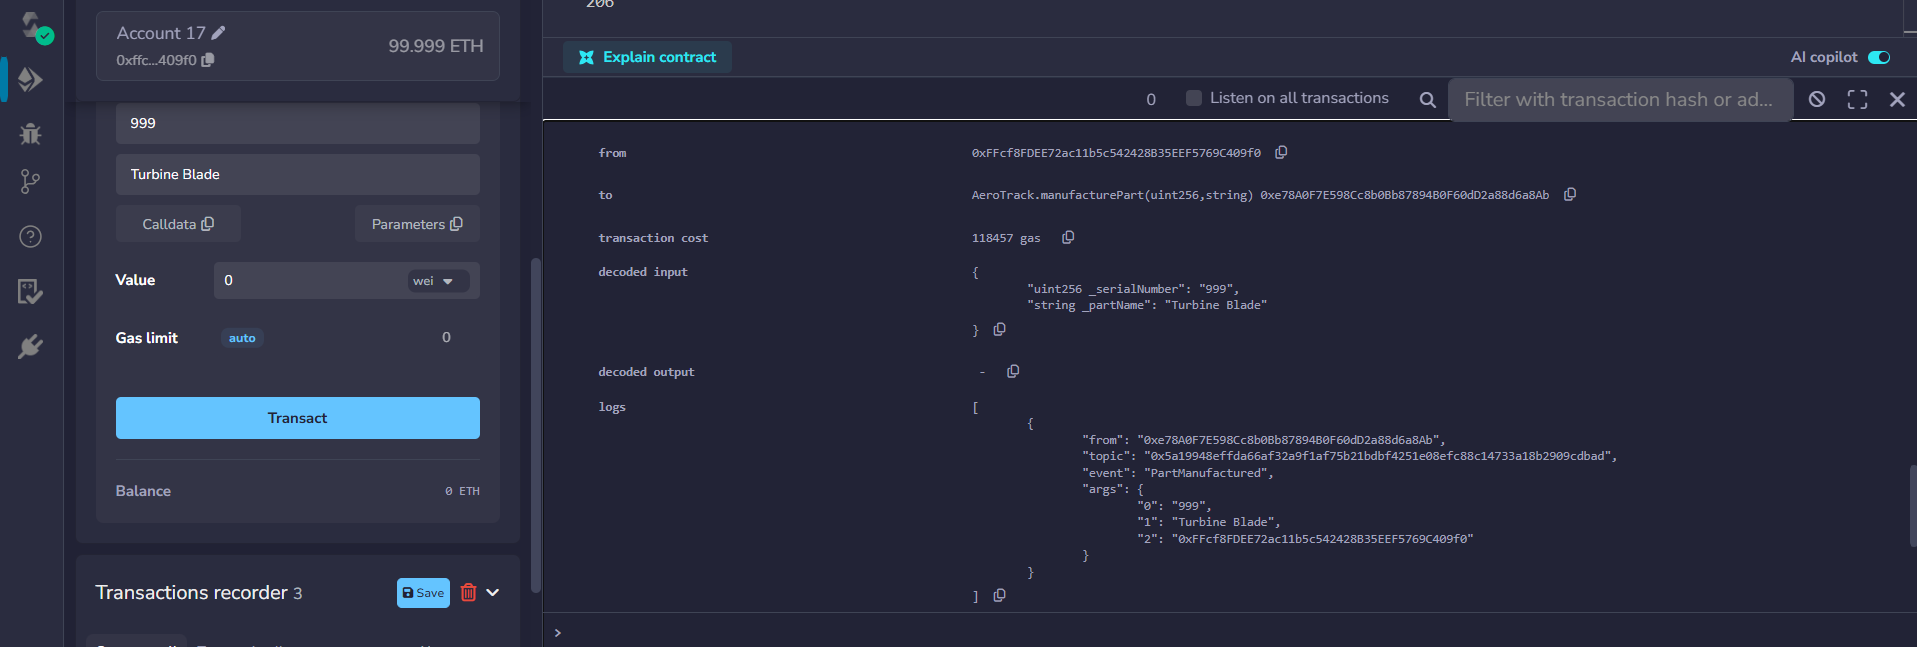
\includegraphics[width=0.85\textwidth]{../screens/step8-registerSensor.png}
    \caption{Registering IoT sensor address on Ganache}
    \label{fig:step8-regsensor}
\end{figure}

\begin{figure}[H]
    \centering
    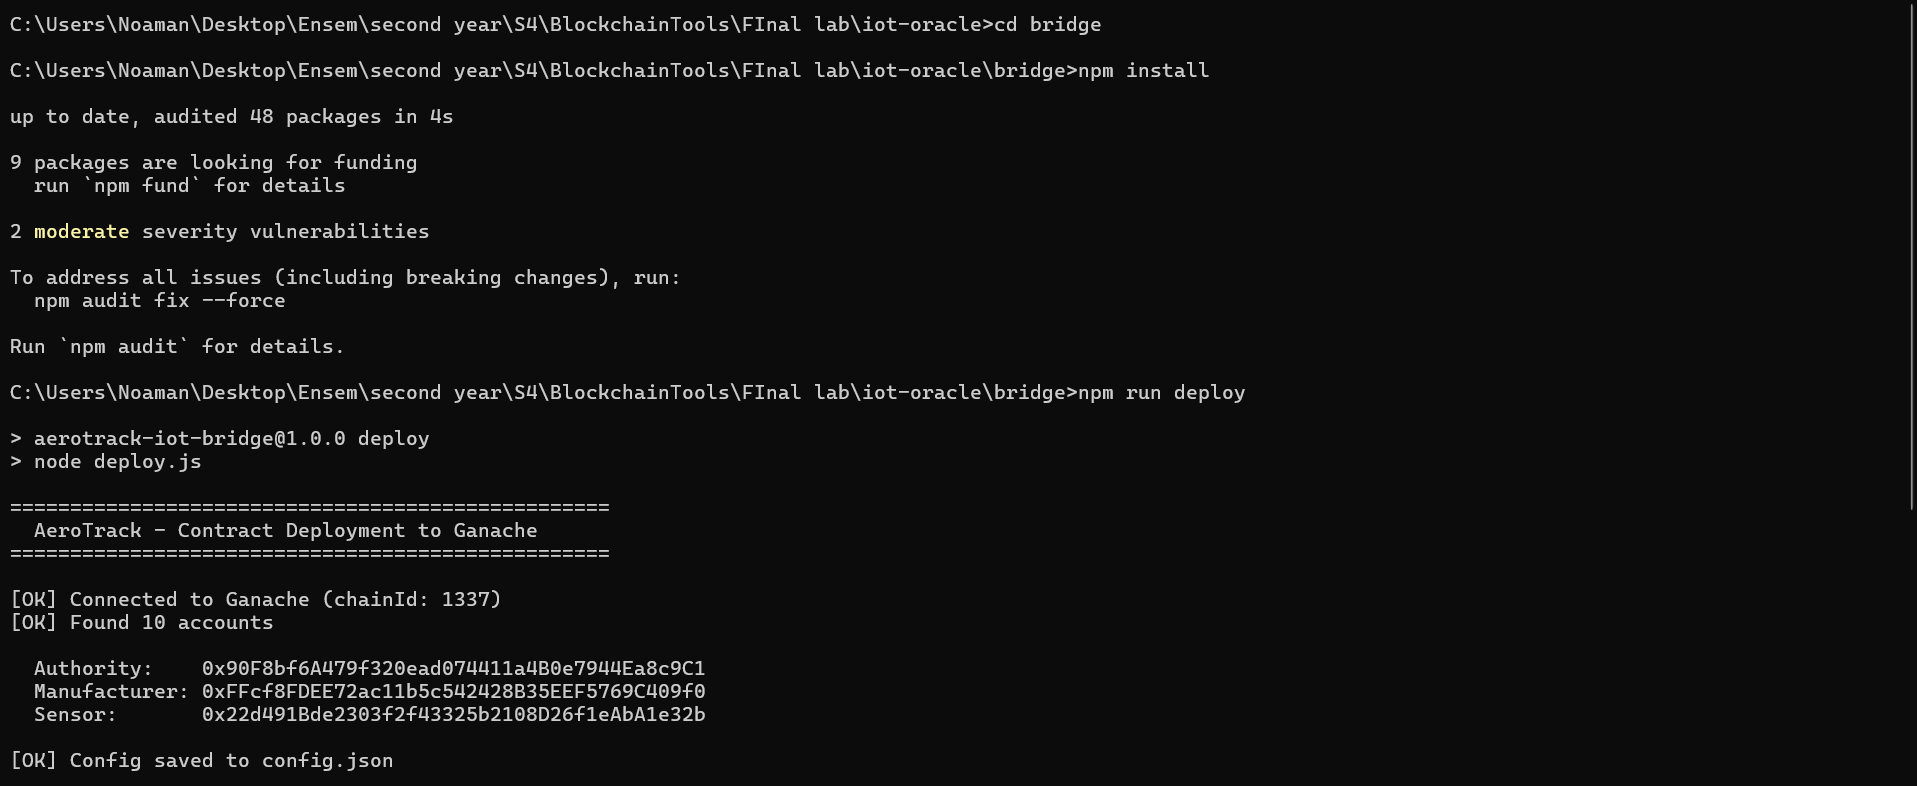
\includegraphics[width=0.85\textwidth]{../screens/step8-npm-deploy.png}
    \caption{Node.js bridge setup: npm install and deploy helper}
    \label{fig:step8-npm}
\end{figure}

\begin{figure}[H]
    \centering
    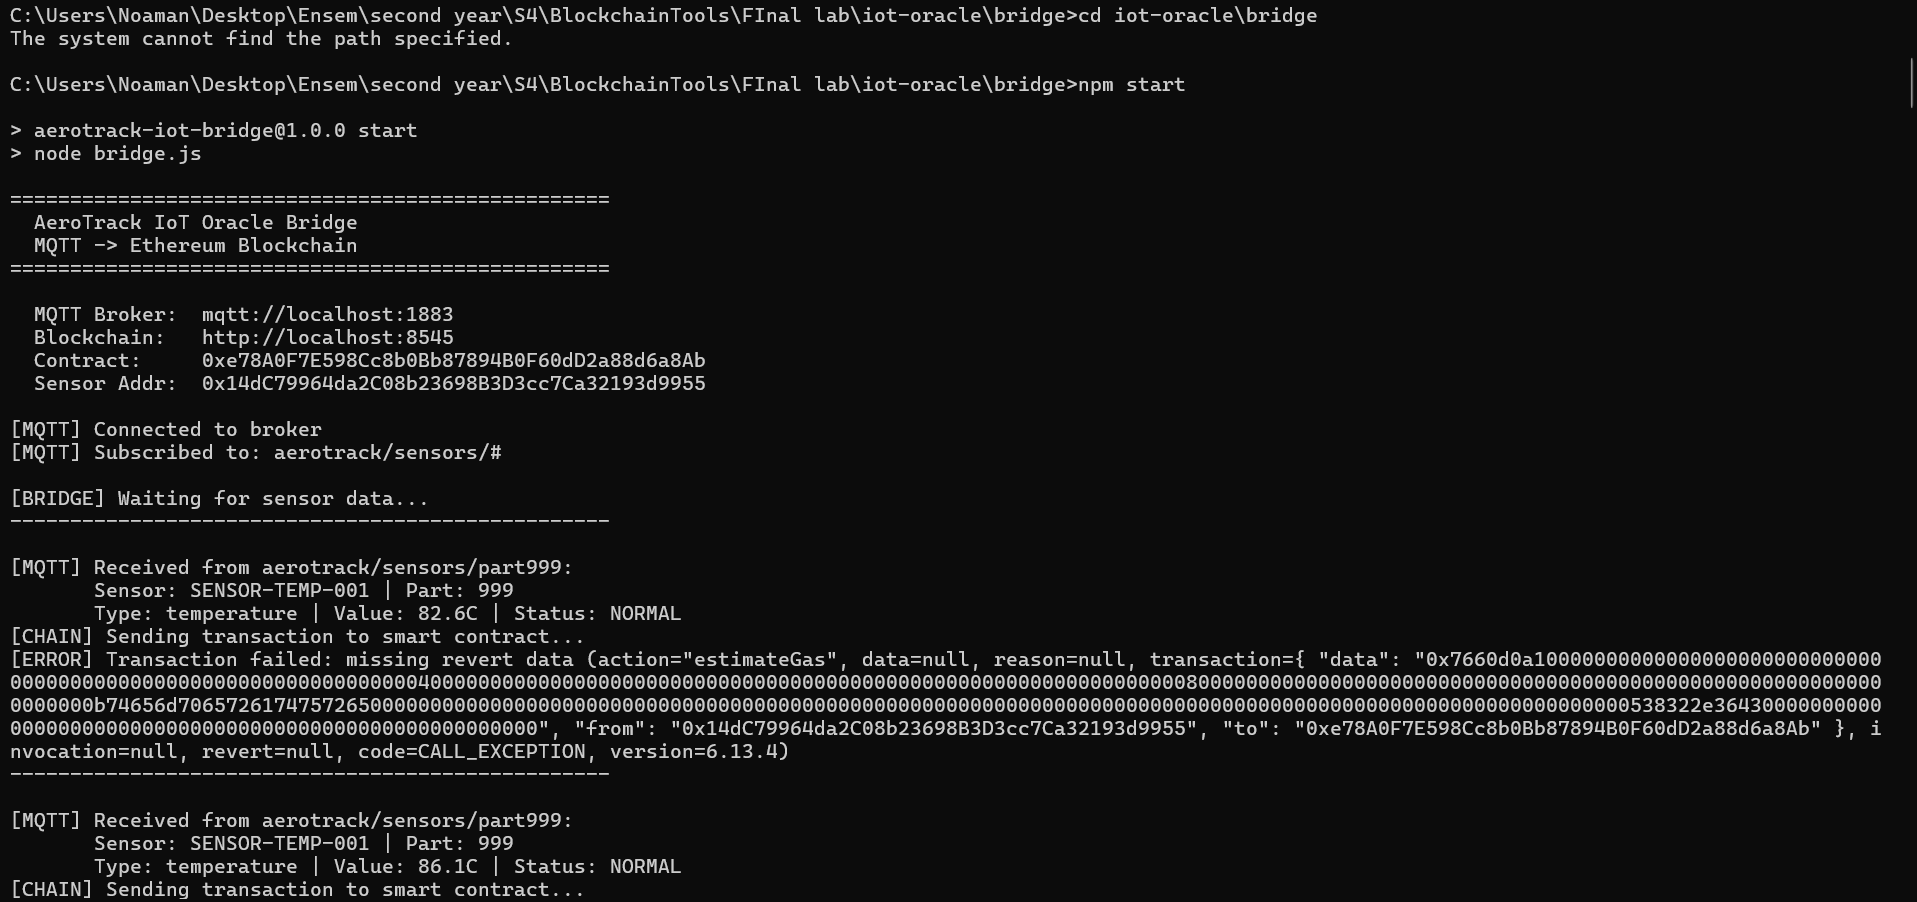
\includegraphics[width=0.85\textwidth]{../screens/step8-bridge-running.png}
    \caption{Bridge running: relaying MQTT messages to blockchain transactions}
    \label{fig:step8-bridge}
\end{figure}

\begin{figure}[H]
    \centering
    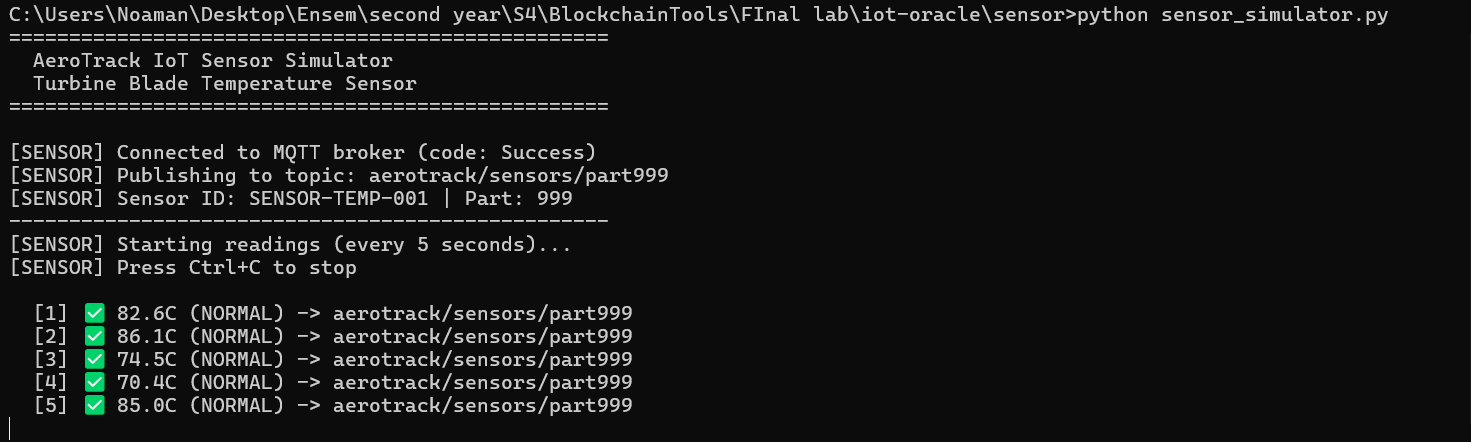
\includegraphics[width=0.85\textwidth]{../screens/step8-sensor-running.png}
    \caption{Python sensor simulator publishing temperature readings via MQTT}
    \label{fig:step8-sensor}
\end{figure}

\begin{figure}[H]
    \centering
    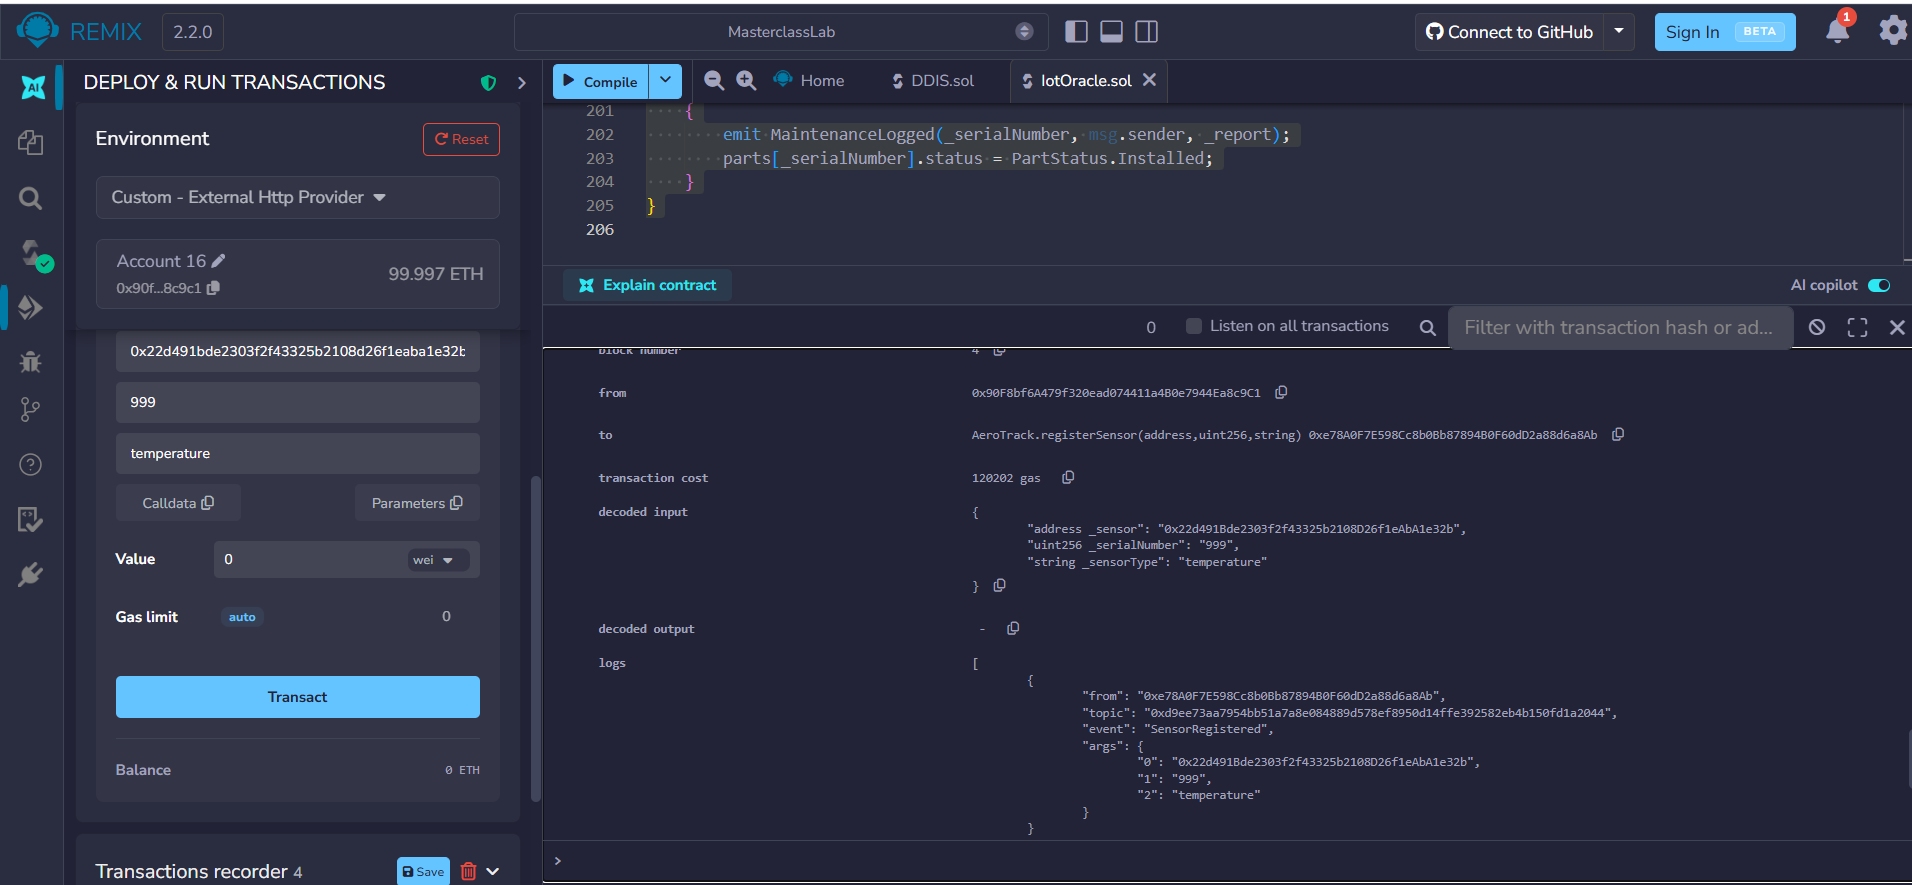
\includegraphics[width=0.85\textwidth]{../screens/step8-remix-events.png}
    \caption{Remix showing SensorDataLogged events from automated MQTT pipeline}
    \label{fig:step8-events}
\end{figure}

% ============================================================
\section{Security and Performance Analysis}
% ============================================================

\subsection{Threat Modeling and Vulnerability Analysis}

In critical industrial sectors like aviation, smart contracts must be protected against malicious inputs and execution failures. We analyzed the AeroTrack contract against standard smart contract security guidelines:

\begin{table}[H]
\centering
\begin{tabularx}{\textwidth}{lXX}
\toprule
\textbf{Threat Vector} & \textbf{Vulnerability Risk} & \textbf{Mitigation in AeroTrack} \\
\midrule
Manufacturer Impersonation & High (Forged parts) & Restricted via the \texttt{onlyCertified} modifier linked to the DID registry. \\
Sensor Data Spoofing & Medium (Faked telemetry) & The \texttt{logSensorData} function resolves the part ID on-chain via the sensor registry, preventing sensors from writing to other parts. \\
Reentrancy Attack & Low (Asset draining) & AeroTrack does not handle value transfers or call external addresses. \\
Integer Overflow/Underflow & Negligible & Mitigated natively by compiling with Solidity \texttt{0.8.19} (checked arithmetic). \\
\bottomrule
\end{tabularx}
\caption{Vulnerability mitigation matrix}
\label{tab:threat-model}
\end{table}

\subsection{Gas Consumption Analysis}

To evaluate the economic efficiency of the AeroTrack protocol, we measured the transaction gas consumption on our local Ganache network (Gas price: 20 Gwei). 

\begin{table}[H]
\centering
\begin{tabularx}{\textwidth}{lrrX}
\toprule
\textbf{Operation} & \textbf{Gas Used} & \textbf{Cost (ETH)} & \textbf{Storage Type} \\
\midrule
Contract Deployment & 1,482,904 & 0.0296 ETH & Contract Creation \\
\texttt{registerManufacturer} & 84,312 & 0.0016 ETH & State Storage (DID) \\
\texttt{manufacturePart} & 112,045 & 0.0022 ETH & State Storage (Struct) \\
\texttt{transferPart} & 28,450 & 0.0005 ETH & State Update (Owner) \\
\texttt{logSensorData} (Event) & 18,912 & 0.0003 ETH & Log Emitted (No Storage) \\
\bottomrule
\end{tabularx}
\caption{Gas usage comparison of various smart contract operations}
\label{tab:gas-analysis}
\end{table}

The data confirms that logging telemetry via events (\texttt{logSensorData}) is approximately \textbf{6 times cheaper} than registering a new part in state storage, justifying the architecture choice for frequent IoT data ingestion.

\subsection{Limitations and Future Work}

While the Node.js MQTT-to-blockchain bridge successfully simulates data transfer, it introduces a \textbf{centralized point of failure} and a single trusted signer. If the bridge server is compromised, fake sensor readings can be written to the blockchain. 

To achieve true decentralization in production, this custom bridge should be replaced with a \textbf{decentralized oracle network} like \textbf{Chainlink Functions}. This ensures multiple independent nodes fetch, verify, and cross-reference MQTT broker readings before executing on-chain transactions.

% ============================================================
\section{Conclusion}
% ============================================================

This project demonstrated how \textbf{Ethereum smart contracts} can secure the provenance of airplane spare parts. The AeroTrack contract implements:

\begin{itemize}
    \item \textbf{Immutable registration} of manufactured parts
    \item \textbf{Role-based access control} via Solidity modifiers
    \item \textbf{Ownership tracking} through the supply chain
    \item \textbf{Gas-efficient traceability} using events
\end{itemize}

% ============================================================
\section*{References}
% ============================================================

\begin{enumerate}
    \item Ethereum Foundation, ``Solidity Documentation,'' \url{https://docs.soliditylang.org/}
    \item Remix IDE, \url{https://remix.ethereum.org/}
    \item EASA, ``Airworthiness Directives and Certificates,'' \url{https://www.easa.europa.eu/}
\end{enumerate}

\newpage
% ============================================================
\appendix
\section{Complete Source Code}
% ============================================================

\subsection{Step 1--4: Base AeroTrack Contract}

\begin{lstlisting}[caption={AeroTrack.sol -- Complete base contract}]
// SPDX-License-Identifier: MIT
pragma solidity ^0.8.19;

contract AeroTrack {

    enum PartStatus { Manufactured, InTransit, Installed, Retired }

    struct Part {
        uint256 serialNumber;
        string partName;
        address manufacturer;
        address currentOwner;
        PartStatus status;
        bool exists;
    }

    address public regulatoryAuthority;
    mapping(uint256 => Part) public parts;

    event PartManufactured(uint256 indexed serialNumber, string partName, address manufacturer);
    event OwnershipTransferred(uint256 indexed serialNumber, address oldOwner, address newOwner);
    event MaintenanceLogged(uint256 indexed serialNumber, address mechanic, string report);

    constructor() {
        regulatoryAuthority = msg.sender;
    }

    modifier partExists(uint256 _serialNumber) {
        require(parts[_serialNumber].exists == true, "Part does not exist.");
        _;
    }

    modifier onlyPartOwner(uint256 _serialNumber) {
        require(parts[_serialNumber].currentOwner == msg.sender, "Not the owner.");
        _;
    }

    function manufacturePart(uint256 _serialNumber, string memory _partName) public {
        require(parts[_serialNumber].exists == false, "Serial Number taken!");
        parts[_serialNumber] = Part({
            serialNumber: _serialNumber,
            partName: _partName,
            manufacturer: msg.sender,
            currentOwner: msg.sender,
            status: PartStatus.Manufactured,
            exists: true
        });
        emit PartManufactured(_serialNumber, _partName, msg.sender);
    }

    function transferPart(uint256 _serialNumber, address _newOwner)
        public partExists(_serialNumber) onlyPartOwner(_serialNumber)
    {
        require(_newOwner != address(0), "Invalid address.");
        address oldOwner = parts[_serialNumber].currentOwner;
        parts[_serialNumber].currentOwner = _newOwner;
        parts[_serialNumber].status = PartStatus.InTransit;
        emit OwnershipTransferred(_serialNumber, oldOwner, _newOwner);
    }

    function logMaintenance(uint256 _serialNumber, string memory _report)
        public partExists(_serialNumber) onlyPartOwner(_serialNumber)
    {
        emit MaintenanceLogged(_serialNumber, msg.sender, _report);
        parts[_serialNumber].status = PartStatus.Installed;
    }
}
\end{lstlisting}

\subsection{Step 5: Certified Manufacturer Registry}

\begin{lstlisting}[caption={Step5\_Enhancement.sol -- Adds certification system}]
// SPDX-License-Identifier: MIT
pragma solidity ^0.8.19;

contract AeroTrack {

    enum PartStatus { Manufactured, InTransit, Installed, Retired }

    struct Part {
        uint256 serialNumber;
        string partName;
        address manufacturer;
        address currentOwner;
        PartStatus status;
        bool exists;
    }

    address public regulatoryAuthority;
    mapping(uint256 => Part) public parts;
    mapping(address => bool) public certifiedManufacturers;

    event PartManufactured(uint256 indexed serialNumber, string partName, address manufacturer);
    event OwnershipTransferred(uint256 indexed serialNumber, address oldOwner, address newOwner);
    event MaintenanceLogged(uint256 indexed serialNumber, address mechanic, string report);
    event ManufacturerCertified(address indexed manufacturer);
    event ManufacturerRevoked(address indexed manufacturer);

    constructor() { regulatoryAuthority = msg.sender; }

    modifier partExists(uint256 _serialNumber) {
        require(parts[_serialNumber].exists == true, "Part does not exist.");
        _;
    }
    modifier onlyPartOwner(uint256 _serialNumber) {
        require(parts[_serialNumber].currentOwner == msg.sender, "Not the owner.");
        _;
    }
    modifier onlyAuthority() {
        require(msg.sender == regulatoryAuthority, "Not the authority.");
        _;
    }
    modifier onlyCertified() {
        require(certifiedManufacturers[msg.sender], "Not a certified manufacturer.");
        _;
    }

    function certifyManufacturer(address _manufacturer) public onlyAuthority {
        require(_manufacturer != address(0), "Invalid address.");
        certifiedManufacturers[_manufacturer] = true;
        emit ManufacturerCertified(_manufacturer);
    }

    function revokeManufacturer(address _manufacturer) public onlyAuthority {
        certifiedManufacturers[_manufacturer] = false;
        emit ManufacturerRevoked(_manufacturer);
    }

    function manufacturePart(uint256 _serialNumber, string memory _partName)
        public onlyCertified
    {
        require(parts[_serialNumber].exists == false, "Serial Number taken!");
        parts[_serialNumber] = Part({
            serialNumber: _serialNumber, partName: _partName,
            manufacturer: msg.sender, currentOwner: msg.sender,
            status: PartStatus.Manufactured, exists: true
        });
        emit PartManufactured(_serialNumber, _partName, msg.sender);
    }

    function transferPart(uint256 _serialNumber, address _newOwner)
        public partExists(_serialNumber) onlyPartOwner(_serialNumber)
    {
        require(_newOwner != address(0), "Invalid address.");
        address oldOwner = parts[_serialNumber].currentOwner;
        parts[_serialNumber].currentOwner = _newOwner;
        parts[_serialNumber].status = PartStatus.InTransit;
        emit OwnershipTransferred(_serialNumber, oldOwner, _newOwner);
    }

    function logMaintenance(uint256 _serialNumber, string memory _report)
        public partExists(_serialNumber) onlyPartOwner(_serialNumber)
    {
        emit MaintenanceLogged(_serialNumber, msg.sender, _report);
        parts[_serialNumber].status = PartStatus.Installed;
    }
}
\end{lstlisting}

\subsection{Step 6: Decentralized Identifiers (DIDs)}

\begin{lstlisting}[caption={Step6\_DIDs.sol -- Adds on-chain identity}]
// SPDX-License-Identifier: MIT
pragma solidity ^0.8.19;

contract AeroTrack {

    enum PartStatus { Manufactured, InTransit, Installed, Retired }

    struct Part {
        uint256 serialNumber; string partName;
        address manufacturer; address currentOwner;
        PartStatus status; bool exists;
    }

    struct ManufacturerIdentity {
        string name; string country; string certificationId;
        bool isActive; uint256 registeredAt;
    }

    address public regulatoryAuthority;
    mapping(uint256 => Part) public parts;
    mapping(address => bool) public certifiedManufacturers;
    mapping(address => ManufacturerIdentity) public manufacturerIdentities;

    event PartManufactured(uint256 indexed serialNumber, string partName, address manufacturer);
    event OwnershipTransferred(uint256 indexed serialNumber, address oldOwner, address newOwner);
    event MaintenanceLogged(uint256 indexed serialNumber, address mechanic, string report);
    event ManufacturerRegistered(address indexed manufacturer, string name, string certificationId);
    event ManufacturerDeactivated(address indexed manufacturer);

    constructor() { regulatoryAuthority = msg.sender; }

    modifier partExists(uint256 _sn) { require(parts[_sn].exists, "Part does not exist."); _; }
    modifier onlyPartOwner(uint256 _sn) { require(parts[_sn].currentOwner == msg.sender, "Not the owner."); _; }
    modifier onlyAuthority() { require(msg.sender == regulatoryAuthority, "Not the authority."); _; }
    modifier onlyCertified() { require(certifiedManufacturers[msg.sender], "Not certified."); _; }

    function registerManufacturer(address _m, string memory _name,
        string memory _country, string memory _certId) public onlyAuthority {
        manufacturerIdentities[_m] = ManufacturerIdentity(_name, _country, _certId, true, block.timestamp);
        certifiedManufacturers[_m] = true;
        emit ManufacturerRegistered(_m, _name, _certId);
    }

    function deactivateManufacturer(address _m) public onlyAuthority {
        manufacturerIdentities[_m].isActive = false;
        certifiedManufacturers[_m] = false;
        emit ManufacturerDeactivated(_m);
    }

    function isManufacturerActive(address _m) public view returns (bool) {
        return manufacturerIdentities[_m].isActive;
    }

    function manufacturePart(uint256 _sn, string memory _name) public onlyCertified {
        require(!parts[_sn].exists, "Serial Number taken!");
        parts[_sn] = Part(_sn, _name, msg.sender, msg.sender, PartStatus.Manufactured, true);
        emit PartManufactured(_sn, _name, msg.sender);
    }

    function transferPart(uint256 _sn, address _new)
        public partExists(_sn) onlyPartOwner(_sn) {
        require(_new != address(0), "Invalid address.");
        address old = parts[_sn].currentOwner;
        parts[_sn].currentOwner = _new;
        parts[_sn].status = PartStatus.InTransit;
        emit OwnershipTransferred(_sn, old, _new);
    }

    function logMaintenance(uint256 _sn, string memory _report)
        public partExists(_sn) onlyPartOwner(_sn) {
        emit MaintenanceLogged(_sn, msg.sender, _report);
        parts[_sn].status = PartStatus.Installed;
    }
}
\end{lstlisting}

\subsection{Step 7: IoT Oracle Simulation}

\begin{lstlisting}[caption={Step7\_IoTOracle.sol -- Adds IoT sensor system}]
// SPDX-License-Identifier: MIT
pragma solidity ^0.8.19;

contract AeroTrack {

    enum PartStatus { Manufactured, InTransit, Installed, Retired }

    struct Part {
        uint256 serialNumber; string partName;
        address manufacturer; address currentOwner;
        PartStatus status; bool exists;
    }

    struct ManufacturerIdentity {
        string name; string country; string certificationId;
        bool isActive; uint256 registeredAt;
    }

    struct Sensor {
        uint256 assignedPart; string sensorType;
        bool isActive; uint256 registeredAt;
    }

    address public regulatoryAuthority;
    mapping(uint256 => Part) public parts;
    mapping(address => bool) public certifiedManufacturers;
    mapping(address => ManufacturerIdentity) public manufacturerIdentities;
    mapping(address => Sensor) public sensors;

    event PartManufactured(uint256 indexed serialNumber, string partName, address manufacturer);
    event OwnershipTransferred(uint256 indexed serialNumber, address oldOwner, address newOwner);
    event MaintenanceLogged(uint256 indexed serialNumber, address mechanic, string report);
    event ManufacturerRegistered(address indexed manufacturer, string name, string certificationId);
    event ManufacturerDeactivated(address indexed manufacturer);
    event SensorRegistered(address indexed sensor, uint256 indexed serialNumber, string sensorType);
    event SensorRevoked(address indexed sensor);
    event SensorDataLogged(uint256 indexed serialNumber, address indexed sensor, string dataType, string value);

    constructor() { regulatoryAuthority = msg.sender; }

    modifier partExists(uint256 _sn) { require(parts[_sn].exists, "Part does not exist."); _; }
    modifier onlyPartOwner(uint256 _sn) { require(parts[_sn].currentOwner == msg.sender, "Not the owner."); _; }
    modifier onlyAuthority() { require(msg.sender == regulatoryAuthority, "Not the authority."); _; }
    modifier onlyCertified() { require(certifiedManufacturers[msg.sender], "Not certified."); _; }
    modifier onlyActiveSensor() { require(sensors[msg.sender].isActive, "Not an authorized sensor."); _; }

    function registerManufacturer(address _m, string memory _name,
        string memory _country, string memory _certId) public onlyAuthority {
        manufacturerIdentities[_m] = ManufacturerIdentity(_name, _country, _certId, true, block.timestamp);
        certifiedManufacturers[_m] = true;
        emit ManufacturerRegistered(_m, _name, _certId);
    }

    function deactivateManufacturer(address _m) public onlyAuthority {
        manufacturerIdentities[_m].isActive = false;
        certifiedManufacturers[_m] = false;
        emit ManufacturerDeactivated(_m);
    }

    function registerSensor(address _sensor, uint256 _sn, string memory _type)
        public onlyAuthority partExists(_sn) {
        require(_sensor != address(0), "Invalid sensor address.");
        sensors[_sensor] = Sensor(_sn, _type, true, block.timestamp);
        emit SensorRegistered(_sensor, _sn, _type);
    }

    function revokeSensor(address _sensor) public onlyAuthority {
        sensors[_sensor].isActive = false;
        emit SensorRevoked(_sensor);
    }

    function logSensorData(string memory _dataType, string memory _value)
        public onlyActiveSensor {
        uint256 sn = sensors[msg.sender].assignedPart;
        emit SensorDataLogged(sn, msg.sender, _dataType, _value);
    }

    function isSensorActive(address _sensor) public view returns (bool) {
        return sensors[_sensor].isActive;
    }

    function manufacturePart(uint256 _sn, string memory _name) public onlyCertified {
        require(!parts[_sn].exists, "Serial Number taken!");
        parts[_sn] = Part(_sn, _name, msg.sender, msg.sender, PartStatus.Manufactured, true);
        emit PartManufactured(_sn, _name, msg.sender);
    }

    function transferPart(uint256 _sn, address _new)
        public partExists(_sn) onlyPartOwner(_sn) {
        require(_new != address(0), "Invalid address.");
        address old = parts[_sn].currentOwner;
        parts[_sn].currentOwner = _new;
        parts[_sn].status = PartStatus.InTransit;
        emit OwnershipTransferred(_sn, old, _new);
    }

    function logMaintenance(uint256 _sn, string memory _report)
        public partExists(_sn) onlyPartOwner(_sn) {
        emit MaintenanceLogged(_sn, msg.sender, _report);
        parts[_sn].status = PartStatus.Installed;
    }
}
\end{lstlisting}

\end{document}
